% ===========================================================================
%  Praca licencjacka
%  Uniwersytet Jagiellonski, WFAIS, kierunek Fizyka dla firm
%  Kompilacja: pdfLaTeX + BibTeX + pdfLaTeX x2  (Overleaf: pdfLaTeX)
% ===========================================================================

\documentclass[12pt,a4paper]{article}

\usepackage[T1]{fontenc}
\usepackage[utf8]{inputenc}
\usepackage[polish]{babel}
\usepackage[a4paper,margin=2.5cm]{geometry}
\usepackage{amsmath,amssymb}
\usepackage{graphicx}
\usepackage{booktabs}
\usepackage{siunitx}
\usepackage{caption}
\usepackage{float}
\usepackage[hidelinks]{hyperref}

\sisetup{output-decimal-marker={,}, group-separator={\,}, detect-weight=true}

\graphicspath{{momentum_sharing_results/figures/}{figures_simplex/}}

\setlength{\parskip}{0.4em}

% Skroty notacyjne
\newcommand{\Neff}{N_{\mathrm{eff}}}
\newcommand{\xmax}{x_{\max}}
\newcommand{\ja}{j.a.}
\newcommand{\PWcm}{PW/cm\textsuperscript{2}}

\title{\textbf{Analiza korelacji pędów trzech elektronów\\
w potrójnej jonizacji neonu w silnym polu laserowym}}
\author{Karina Nepravskaya}
\date{Kraków \the\year}

\begin{document}

\maketitle

\begin{abstract}
\noindent
Praca dotyczy sposobu opisu podziału pędu pomiędzy trzy elektrony
uwalniane w niesekwencyjnej potrójnej jonizacji neonu w silnym polu
laserowym. Analizowane są pędy końcowe pochodzące z
półklasycznego modelu ECBB. Punktem wyjścia jest reprezentacja
simpleksowa, która dobrze działa dla trzech składowych, ale przestaje
być czytelna przy większej ich liczbie. Jako opis alternatywny zaproponowano wprowadzić
stałą bazę ortonormalną rozdzielającą ruch kolektywny od
ruchu względnego oraz zestaw skalarnych obserwabli podziału pędu.
Bazę wybrano na podstawie analizy składowych głównych, ale nie
utożsamiono jej z osiami PCA. Pokazano, że obserwable te odtwarzają
ilościowo wnioski uzyskane wcześniej metodą simpleksową, a
dodatkowo rozdzielają kanały \emph{direct} i \emph{delayed} oraz
ujawniają asymetrię związaną ze sposobem etykietowania
elektronów. W odróżnieniu od reprezentacji simpleksowej proponowany opis
nie traci czytelności przy większej liczbie elektronów.
\end{abstract}

\tableofcontents
\newpage

% ===========================================================================
% предварительно ОК
\section{Wstęp}
% ===========================================================================

\subsection{Jonizacja atomów w silnym polu laserowym}

Gdy natężenie pola laserowego staje się porównywalne z polem
wiążącym elektrony w atomie, opis jonizacji jako absorpcji
pojedynczych fotonów przestaje wystarczać. Pole zewnętrzne obniża
barierę potencjału na tyle, że elektron może się przez nią
przetunelować~\cite{Ammosov1986}. Elektron uwolniony w odpowiedniej fazie pola jest początkowo oddalany od jonu, lecz po zmianie zwrotu pola może zostać zawrócony i ponownie zbliżyć się do jonu macierzystego. Mechanizm ten, nazywany rekolizją, może prowadzić do niesekwencyjnej jonizacji wielokrotnej, w której kilka elektronów opuszcza atom w sposób skorelowany~\cite{Corkum1993}.

Jednym z podstawowych doświadczalnych sygnałów niesekwencyjnej jonizacji wielokrotnej jest nadmiar jonów wielokrotnie naładowanych w stosunku do przewidywań modelu jonizacji sekwencyjnej~\cite{LHuillier1983,BeckerRottke2008}.
Pomiary koincydencyjne pokazały, że informacja o mechanizmie zapisana jest
nie w widmie pojedynczego elektronu, lecz w \emph{korelacjach} między
pędami elektronów~\cite{Moshammer2000,Rudenko2004,Rudenko2007}.
Dla dwóch elektronów standardowym narzędziem jest dwuwymiarowy rozkład
$(p_{1z},p_{2z})$ składowych wzdłuż osi polaryzacji. Dla trzech i więcej
elektronów taki bezpośredni wykres przestaje być możliwy i konieczna
jest świadomie wybrana reprezentacja danych.

\subsection{Reprezentacja simpleksowa podziału pędu}

Naturalnym rozwiązaniem dla trzech elektronów jest reprezentacja
simpleksowa, znana w fizyce cząstek jako wykres
Dalitza~\cite{Dalitz1953}. Zamiast trzech pędów rozpatruje się ich
udziały w całkowitym pędzie bezwzględnym. Trzy liczby nieujemne
sumujące się do jedności można przedstawić jako współrzędne
barycentryczne punktu w trójkącie równobocznym. Środek trójkąta
odpowiada równemu podziałowi pędu, wierzchołki -- sytuacji, w której
cały pęd niesie jeden elektron.

Takie podejście zastosował Ojczenasz~\cite{Ojczenasz2023} do tych samych
danych, które analizowane są w niniejszej pracy. Znaki pędów
zapisano tam osobno: osiem kombinacji znaków trzech składowych
podłużnych odpowiada ośmiu ścianom ośmiościanu, rozwiniętym na
płaszczyźnie jako osiem trójkątów. Metoda ta pozwoliła
zaobserwować, że przy emisji wszystkich trzech elektronów w tę
samą stronę pęd dzieli się w przybliżeniu równomiernie,
natomiast gdy jeden elektron porusza się przeciwnie do pozostałych,
niesie on małą część pędu.

\subsection{Problem skalowalności i cel pracy}

Reprezentacja simpleksowa działa dobrze dla trzech składowych, ponieważ
zbiór punktów o ustalonej sumie tworzy wówczas dwuwymiarowy trójkąt.
Dla czterech składowych odpowiednikiem jest czworościan, a dla większej
liczby elektronów simpleks o coraz wyższym wymiarze. Już dla czterech elektronów konieczna staje się analiza trójwymiarowej reprezentacji danych z wykorzystaniem kodowania barwnego i/lub przekrojów, co znacznie utrudnia interpretację wyników.
Rośnie również liczba sektorów znakowych, ponieważ dla $N$ elektronów jest ich
$2^{N}$, czyli osiem dla trzech i szesnaście dla czterech elektronów.

Celem pracy jest zbudowanie i sprawdzenie opisu korelacji pędów, który
zachowuje interpretację fizyczną reprezentacji simpleksowej, ale nie
opiera się na analizie obiektu geometrycznego o wymiarze rosnącym
z liczbą elektronów. Zamiast tego używane są wielkości skalarne,
które dla dowolnej liczby elektronów pozostają liczbami i mogą
być przedstawiane na zwykłych histogramach. Praca odpowiada na trzy
pytania:

\begin{enumerate}
  \item Czy zaproponowane obserwable odtwarzają wnioski uzyskane
        metodą simpleksową na tych samych danych?
  \item Czy pozwalają rozróżnić kanały \emph{direct} i
        \emph{delayed} przy ustalonej intensywności pola?
  \item Co tracą, a co zyskują w porównaniu z reprezentacją
        simpleksową?
\end{enumerate}

Struktura pracy odpowiada tym pytaniom. W rozdziale~\ref{sec:dane} opisano
dane, w rozdziale~\ref{sec:metoda} metodę wraz z jej sprawdzeniem,
w rozdziale~\ref{sec:wyniki} wyniki, a w rozdziale~\ref{sec:porownanie}
porównanie z metodą simpleksową.

% ===========================================================================
\section{Dane}
\label{sec:dane}
% ===========================================================================

\subsection{Model ECBB i parametry impulsów}

Analizowane dane pochodzą z półklasycznych obliczeń opisanych w
pracy Emmanouilidou, Petersa i Katsoulisa~\cite{Emmanouilidou2023} i
udostępnionych wraz z nią. Model, oznaczany skrótem ECBB, opisuje
układ czterech ciał: rdzenia jonowego i trzech elektronów. W trakcie
propagacji każdy elektron jest na bieżąco klasyfikowany jako
związany albo kwazi-swobodny. Oddziaływania rdzeń--elektron oraz
oddziaływanie elektronu powracającego z elektronem związanym
zachowują pełną osobliwość kulombowską. Zmiękczony
potencjał efektywny stosowany jest wyłącznie między parą
elektronów związanych; zapobiega to niefizycznej autojonizacji, czyli
sytuacji, w której jeden elektron spada do głęboko ujemnych energii
i wyrzuca pozostałe~\cite{Emmanouilidou2023,Peters2022}.

Pole laserowe jest spolaryzowane liniowo wzdłuż osi $z$. Czas trwania
impulsu wynosi \num{25}~fs. Parametry czterech dostępnych zbiorów zebrano
w~tabeli~\ref{tab:impulsy}. Wraz z nimi podano energię ponderomotoryczną
$U_p=E_0^2/(4\omega^2)$ oraz odpowiadającą jej charakterystyczną skalę pędu elektronu uwolnionego w silnym polu $2\sqrt{U_p}=E_0/\omega$.

\begin{table}[H]
\centering
\caption{Parametry analizowanych impulsów laserowych. Wartości $U_p$ i
$2\sqrt{U_p}$ podano w jednostkach atomowych. Zbiór o intensywności
\num{1.7}~\PWcm{} został policzony dla innej długości fali niż
pozostałe trzy.}
\label{tab:impulsy}
\begin{tabular}{ccccc}
\toprule
$I$ [\PWcm] & $\lambda$ [nm] & $\omega$ [\ja] & $U_p$ [\ja] & $2\sqrt{U_p}$ [\ja] \\
\midrule
\num{1.0} & \num{800} & \num{0.0570} & \num{2.196} & \num{2.964} \\
\num{1.3} & \num{800} & \num{0.0570} & \num{2.855} & \num{3.379} \\
\num{1.6} & \num{800} & \num{0.0570} & \num{3.514} & \num{3.749} \\
\num{1.7} & \num{760} & \num{0.0600} & \num{3.369} & \num{3.671} \\
\bottomrule
\end{tabular}
\end{table}

Różnica długości fali dla zbioru \num{1.7}~\PWcm{} jest istotna
metodologicznie. Zmiana $\lambda$ zmienia $U_p$ przy ustalonej
intensywności, więc tego zbioru nie można traktować jako czwartego
punktu jednej serii pomiarowej. W dalszej części pracy serię
intensywności tworzą zbiory \num{1.0}, \num{1.3} i \num{1.6}~\PWcm{}
przy \num{800}~nm, a zbiór \num{1.7}~\PWcm{} przy \num{760}~nm służy
wyłącznie jako niezależne sprawdzenie powtarzalności wniosków.

\subsection{Format danych i etykietowanie cząstek}

Każdy wiersz pliku wejściowego opisuje jedno zdarzenie i zawiera
dwanaście liczb: trzy składowe kartezjańskie pędu końcowego dla
czterech cząstek, w kolejności
$p_{1x}$, $p_{1y}$, $p_{1z}$, \dots, $p_{4x}$, $p_{4y}$, $p_{4z}$. Cząstka 1 to rdzeń
jonowy, cząstki 2 i 3 to elektrony początkowo związane, a
cząstka 4 to elektron początkowo tunelujący. Wszystkie wielkości
podane są w jednostkach atomowych.

Etykiety te mają charakter techniczny. Opisują rolę danej
trajektorii w mechanizmie jonizacji przyjętym w modelu, a nie własność
fizyczną cząstki. Elektrony są nierozróżnialne, więc numer
elektronu nie jest wielkością obserwowalną. W modelu ECBB podział
na elektrony związane i kwazi-swobodne zmienia się zresztą w czasie
propagacji~\cite{Emmanouilidou2023}. W całej pracy konsekwentnie
rozdzielono zatem dwa poziomy opisu: wielkości niezależne od numeracji,
które mogą być interpretowane fizycznie, oraz wielkości zależne od
numeracji, które traktowane są jako informacja o samym modelu.

Ponieważ pole laserowe jest spolaryzowane wzdłuż osi \(z\), analizę ograniczono do składowych pędu $p_{2z},p_{3z},p_{4z}$ równoległych do tej osi, które bezpośrednio odzwierciedlają dynamikę elektronów napędzaną przez pole. Składowe poprzeczne nie są przedmiotem dalszej analizy. Dla skrócenia zapisu
przyjęto oznaczenia
\begin{equation}
p_2 \equiv p_{2z},\qquad p_3 \equiv p_{3z},\qquad p_4 \equiv p_{4z}.
\end{equation}

\subsection{Kanały \emph{direct} i \emph{delayed}}

Dla każdej intensywności dostępne są trzy pliki: wszystkie
zdarzenia oraz dwa główne kanały. W kanale \emph{direct}, oznaczanym
$(e,3e)$, wszystkie trzy elektrony jonizują się wkrótce po
rekolizji. W kanale \emph{delayed}, oznaczanym $(e,2e)$, powracający
elektron przekazuje energię wystarczającą do jonizacji tylko dwóch
elektronów, a trzeci opuszcza atom z opóźnieniem. Liczbę zdarzeń w poszczególnych zbiorach podano w tabeli~\ref{tab:licznosci}.

\begin{table}[H]
\centering
\caption{Liczba zdarzeń w analizowanych zbiorach oraz udział kanałów w
zbiorze wszystkich zdarzeń. Udziały wyznaczono bezpośrednio z liczby
wierszy w plikach.}
\label{tab:licznosci}
\begin{tabular}{cccccc}
\toprule
$I$ [\PWcm] & wszystkie & \emph{direct} & \emph{delayed} &
udział \emph{direct} & udział \emph{delayed} \\
\midrule
\num{1.0} & \num{4872}  & \num{2042} & \num{2097} & \num{41.9}\,\% & \num{43.0}\,\% \\
\num{1.3} & \num{13769} & \num{6198} & \num{5837} & \num{45.0}\,\% & \num{42.4}\,\% \\
\num{1.6} & \num{18578} & \num{8799} & \num{7560} & \num{47.4}\,\% & \num{40.7}\,\% \\
\num{1.7} & \num{3873}  & \num{1695} & \num{1601} & \num{43.8}\,\% & \num{41.3}\,\% \\
\bottomrule
\end{tabular}
\end{table}

Wartości udziałów kanałów obliczono na podstawie liczby zdarzeń w poszczególnych plikach. Dla zbioru przy \(\num{1.7}\)~\PWcm{} stwierdzono niezgodność między wyznaczonym udziałem kanału \emph{direct} a wartością podaną w dokumentacji danych. W związku z tym w całej pracy wykorzystano udziały obliczone bezpośrednio z plików.

Dodatkowo, suma obu kanałów nie wyczerpuje zbioru wszystkich zdarzeń. Oba kanały
opisują ścieżki główne, a pozostałe kilkanaście procent
zdarzeń przypisane jest ścieżkom rzadszym. Z tego powodu zbiór
wszystkich zdarzeń nie jest dokładnie sumą dwóch kanałów i
analizowany jest osobno.

% ===========================================================================
\section{Metoda analizy}
\label{sec:metoda}
% ===========================================================================

%is OK
\subsection{Analiza składowych głównych}
\label{sec:pca}

Przed wyborem współrzędnych sprawdzono, jakie kierunki w przestrzeni
pędów są wyróżnione przez same dane. W tym celu wykonano
analizę składowych głównych (PCA)~\cite{Jolliffe2002} dla wszystkich
dwunastu zbiorów. Wektorem wejściowym było dziewięć składowych
pędu trzech elektronów,
\begin{equation}
(p_{2x},p_{2y},p_{2z},\;p_{3x},p_{3y},p_{3z},\;p_{4x},p_{4y},p_{4z}),
\end{equation}
a każdą składową wystandaryzowano przed rozkładem, co odpowiada
analizie macierzy korelacji. Pęd rdzenia nie był używany.

Gdyby wszystkie dziewięć składowych było nieskorelowanych i
równoważnych, każda składowa główna wyjaśniałaby
\num{11.1}\,\% wariancji. Otrzymany rozkład jest wyraźnie inny.
Przykładowo, przy natężeniu \num{1.3}~\PWcm{} pierwsza składowa
główna wyjaśnia \num{29.9}\,\% wariancji w kanale \emph{direct}
i \num{19.8}\,\% w kanale \emph{delayed}. Dwie ostatnie składowe
wyjaśniają odpowiednio \num{2.0}\,\% i \num{1.4}\,\% oraz
\num{8.1}\,\% i \num{5.4}\,\%. Analogiczny układ występuje przy
pozostałych intensywnościach, co pokazano w
tabeli~\ref{tab:pca_wariancja}.

\begin{table}[H]
\centering
\small
\setlength{\tabcolsep}{4.5pt}
\caption{Wariancja wyjaśniona przez składowe PC1, PC8 i PC9
dla wszystkich analizowanych intensywności i kanałów.}
\label{tab:pca_wariancja}
\begin{tabular}{c ccc ccc ccc}
\toprule
& \multicolumn{3}{c}{\emph{direct}}
& \multicolumn{3}{c}{\emph{delayed}}
& \multicolumn{3}{c}{wszystkie zdarzenia} \\
\cmidrule(lr){2-4}
\cmidrule(lr){5-7}
\cmidrule(lr){8-10}
$I$ [\PWcm]
& PC1 & PC8 & PC9
& PC1 & PC8 & PC9
& PC1 & PC8 & PC9 \\
\midrule
\num{1.0} & \num{30.0}\,\% & \num{1.9}\,\% & \num{1.5}\,\% & \num{19.2}\,\% & \num{8.1}\,\% & \num{5.9}\,\% & \num{23.9}\,\% & \num{4.9}\,\% & \num{4.5}\,\% \\
\num{1.3} & \num{29.9}\,\% & \num{2.0}\,\% & \num{1.4}\,\% & \num{19.8}\,\% & \num{8.1}\,\% & \num{5.4}\,\% & \num{24.7}\,\% & \num{4.5}\,\% & \num{4.1}\,\% \\
\num{1.6} & \num{29.7}\,\% & \num{2.3}\,\% & \num{1.4}\,\% & \num{20.1}\,\% & \num{8.1}\,\% & \num{5.1}\,\% & \num{25.0}\,\% & \num{4.3}\,\% & \num{4.0}\,\% \\
\num{1.7} & \num{29.7}\,\% & \num{2.3}\,\% & \num{1.5}\,\% & \num{19.4}\,\% & \num{8.6}\,\% & \num{5.2}\,\% & \num{24.2}\,\% & \num{4.8}\,\% & \num{4.3}\,\% \\
\bottomrule
\end{tabular}
\end{table}

Istotne jest, że dla składowych PC1, PC8 i PC9 kwadrat normy współczynników przypadający na składowe podłużne wynosi od \num{0.899} do wartości bliskich jedności, a w większości analizowanych zbiorów przekracza \num{0.99} (tabela~\ref{tab:pca_podluzne}). Oznacza to, że te kierunki leżą niemal w całości w podprzestrzeni $(p_{2z},p_{3z},p_{4z})$.

\begin{table}[H]
\centering
\small
\setlength{\tabcolsep}{4pt}
\caption{Kwadrat normy współczynników składowych PC1, PC8 i PC9
przypadający na składowe podłużne $p_{2z}$, $p_{3z}$ i $p_{4z}$.}
\label{tab:pca_podluzne}
\begin{tabular}{c ccc ccc ccc}
\toprule
& \multicolumn{3}{c}{\emph{direct}}
& \multicolumn{3}{c}{\emph{delayed}}
& \multicolumn{3}{c}{wszystkie zdarzenia} \\
\cmidrule(lr){2-4}
\cmidrule(lr){5-7}
\cmidrule(lr){8-10}
$I$ [\PWcm]
& PC1 & PC8 & PC9
& PC1 & PC8 & PC9
& PC1 & PC8 & PC9 \\
\midrule
\num{1.0}
& \num{0.996} & \num{0.999} & \num{1.000}
& \num{0.987} & \num{0.968} & \num{0.980}
& \num{0.996} & \num{0.999} & \num{0.996} \\
\num{1.3}
& \num{1.000} & \num{1.000} & \num{1.000}
& \num{0.998} & \num{0.983} & \num{0.999}
& \num{1.000} & \num{1.000} & \num{1.000} \\
\num{1.6}
& \num{0.998} & \num{1.000} & \num{1.000}
& \num{0.997} & \num{0.990} & \num{0.999}
& \num{0.998} & \num{1.000} & \num{1.000} \\
\num{1.7}
& \num{0.996} & \num{0.999} & \num{0.999}
& \num{0.996} & \num{0.899} & \num{0.994}
& \num{0.999} & \num{0.998} & \num{0.999} \\
\bottomrule
\end{tabular}
\end{table}


Współczynniki tych trzech składowych układają się we wszystkich
dwunastu zbiorach w ten sam sposób. Dla PC1 wszystkie trzy
współczynniki są dodatnie i niemal równe. Ich suma zawiera się
między \num{1.717} a \num{1.732}, wobec $\sqrt3\approx\num{1.732}$
dla współczynników dokładnie równych. Dla PC8 i PC9 współczynniki
mają różne znaki, a moduł ich sumy nie przekracza \num{0.148}.
Wskazuje to na jeden kierunek kolektywny oraz prostopadłą do niego
dwuwymiarową podprzestrzeń opisującą różnice między pędami.
Kierunki te zapisano w postaci dokładnej, symetrycznej względem
numeracji elektronów:

\begin{equation}
\mathbf{e}_0=\frac{1}{\sqrt3}(1,1,1),\qquad
\mathbf{e}_1=\frac{1}{\sqrt2}(1,-1,0),\qquad
\mathbf{e}_2=\frac{1}{\sqrt6}(1,1,-2).
\label{eq:baza}
\end{equation}
Są to pierwsze trzy wiersze macierzy Helmerta~\cite{Lancaster1965},
standardowej konstrukcji rozdzielającej wartość średnią od odchyleń
od niej. Kierunek $\mathbf{e}_0$ odpowiada zgodnej zmianie wszystkich
trzech pędów podłużnych, $\mathbf{e}_1$ opisuje różnicę pędów dwóch
elektronów początkowo związanych, a $\mathbf{e}_2$ zestawia tę parę
z elektronem tunelującym.

Tabela~\ref{tab:pca} zestawia unormowane współczynniki podłużne
składowych PC1, PC8 i PC9 oraz ich zgodność z kierunkami
$\mathbf{e}_0$, $\mathbf{e}_1$ i $\mathbf{e}_2$, mierzoną wartością
bezwzględną iloczynu skalarnego, dla wszystkich dwunastu zbiorów.

\begin{table}[!h]
\centering
\footnotesize
\setlength{\tabcolsep}{4pt}
\caption{Unormowane współczynniki składowych PC1, PC8 i PC9 w
podprzestrzeni podłużnej $(p_{2z},p_{3z},p_{4z})$ oraz wartość
bezwzględna ich iloczynu skalarnego z kierunkami
odniesienia~\eqref{eq:baza}. Znak wektora własnego jest w analizie
składowych głównych dowolny. Ustalono go tak, aby pierwszy niezerowy
współczynnik był dodatni.}
\label{tab:pca}
\begin{tabular}{c l c ccc ccc}
\toprule
& & & \multicolumn{3}{c}{współczynniki unormowane}
    & \multicolumn{3}{c}{$|$iloczyn skalarny$|$} \\
\cmidrule(lr){4-6}
\cmidrule(lr){7-9}
$I$ [\PWcm] & kanał & PC & $c_2$ & $c_3$ & $c_4$
& $\mathbf{e}_0$ & $\mathbf{e}_1$ & $\mathbf{e}_2$ \\
\midrule
\num{1.0} & \emph{direct} & PC1 & \num{0.581} & \num{0.578} & \num{0.573} & \num{1.000} & \num{0.002} & \num{0.005} \\
 &  & PC8 & \num{0.283} & \num{0.517} & \num{-0.808} & \num{0.005} & \num{0.165} & \num{0.986} \\
 &  & PC9 & \num{0.763} & \num{-0.631} & \num{-0.136} & \num{0.003} & \num{0.986} & \num{0.165} \\
\midrule
\num{1.0} & \emph{delayed} & PC1 & \num{0.566} & \num{0.539} & \num{0.624} & \num{0.998} & \num{0.020} & \num{0.058} \\
 &  & PC8 & \num{0.620} & \num{-0.777} & \num{0.107} & \num{0.029} & \num{0.988} & \num{0.151} \\
 &  & PC9 & \num{0.537} & \num{0.333} & \num{-0.775} & \num{0.055} & \num{0.144} & \num{0.988} \\
\midrule
\num{1.0} & wszystkie & PC1 & \num{0.581} & \num{0.573} & \num{0.579} & \num{1.000} & \num{0.005} & \num{0.002} \\
 &  & PC8 & \num{0.339} & \num{-0.817} & \num{0.467} & \num{0.006} & \num{0.817} & \num{0.576} \\
 &  & PC9 & \num{0.741} & \num{-0.075} & \num{-0.668} & \num{0.001} & \num{0.577} & \num{0.817} \\
\midrule
\num{1.3} & \emph{direct} & PC1 & \num{0.580} & \num{0.581} & \num{0.571} & \num{1.000} & \num{0.001} & \num{0.007} \\
 &  & PC8 & \num{0.434} & \num{0.374} & \num{-0.820} & \num{0.007} & \num{0.042} & \num{0.999} \\
 &  & PC9 & \num{0.690} & \num{-0.723} & \num{0.035} & \num{0.001} & \num{0.999} & \num{0.042} \\
\midrule
\num{1.3} & \emph{delayed} & PC1 & \num{0.542} & \num{0.557} & \num{0.630} & \num{0.998} & \num{0.010} & \num{0.065} \\
 &  & PC8 & \num{0.737} & \num{-0.674} & \num{-0.037} & \num{0.015} & \num{0.998} & \num{0.056} \\
 &  & PC9 & \num{0.406} & \num{0.483} & \num{-0.776} & \num{0.065} & \num{0.055} & \num{0.996} \\
\midrule
\num{1.3} & wszystkie & PC1 & \num{0.574} & \num{0.576} & \num{0.582} & \num{1.000} & \num{0.002} & \num{0.005} \\
 &  & PC8 & \num{0.761} & \num{-0.637} & \num{-0.120} & \num{0.002} & \num{0.989} & \num{0.148} \\
 &  & PC9 & \num{0.302} & \num{0.511} & \num{-0.805} & \num{0.005} & \num{0.148} & \num{0.989} \\
\midrule
\num{1.6} & \emph{direct} & PC1 & \num{0.582} & \num{0.582} & \num{0.568} & \num{1.000} & \num{0.000} & \num{0.011} \\
 &  & PC8 & \num{0.400} & \num{0.404} & \num{-0.823} & \num{0.011} & \num{0.003} & \num{1.000} \\
 &  & PC9 & \num{0.708} & \num{-0.706} & \num{-0.002} & \num{0.000} & \num{1.000} & \num{0.003} \\
\midrule
\num{1.6} & \emph{delayed} & PC1 & \num{0.549} & \num{0.546} & \num{0.633} & \num{0.998} & \num{0.002} & \num{0.070} \\
 &  & PC8 & \num{0.699} & \num{-0.715} & \num{0.009} & \num{0.004} & \num{1.000} & \num{0.013} \\
 &  & PC9 & \num{0.455} & \num{0.439} & \num{-0.775} & \num{0.069} & \num{0.011} & \num{0.998} \\
\midrule
\num{1.6} & wszystkie & PC1 & \num{0.576} & \num{0.575} & \num{0.581} & \num{1.000} & \num{0.000} & \num{0.004} \\
 &  & PC8 & \num{0.701} & \num{-0.713} & \num{0.011} & \num{0.000} & \num{1.000} & \num{0.014} \\
 &  & PC9 & \num{0.421} & \num{0.401} & \num{-0.814} & \num{0.005} & \num{0.014} & \num{1.000} \\
\midrule
\num{1.7} & \emph{direct} & PC1 & \num{0.582} & \num{0.582} & \num{0.569} & \num{1.000} & \num{0.000} & \num{0.010} \\
 &  & PC8 & \num{0.403} & \num{0.402} & \num{-0.822} & \num{0.010} & \num{0.000} & \num{1.000} \\
 &  & PC9 & \num{0.707} & \num{-0.707} & \num{0.001} & \num{0.001} & \num{1.000} & \num{0.001} \\
\midrule
\num{1.7} & \emph{delayed} & PC1 & \num{0.546} & \num{0.534} & \num{0.646} & \num{0.996} & \num{0.008} & \num{0.086} \\
 &  & PC8 & \num{0.680} & \num{-0.733} & \num{0.032} & \num{0.012} & \num{0.999} & \num{0.048} \\
 &  & PC9 & \num{0.481} & \num{0.431} & \num{-0.764} & \num{0.086} & \num{0.036} & \num{0.996} \\
\midrule
\num{1.7} & wszystkie & PC1 & \num{0.576} & \num{0.571} & \num{0.585} & \num{1.000} & \num{0.004} & \num{0.009} \\
 &  & PC8 & \num{0.619} & \num{-0.772} & \num{0.143} & \num{0.005} & \num{0.984} & \num{0.179} \\
 &  & PC9 & \num{0.533} & \num{0.280} & \num{-0.798} & \num{0.008} & \num{0.179} & \num{0.984} \\
\bottomrule
\end{tabular}
\end{table}

Wynik ten prowadzi do dwóch wniosków. Po pierwsze, dane wyróżniają
jeden kierunek kolektywny, wzdłuż którego wszystkie trzy pędy
podłużne zmieniają się zgodnie. Współczynniki PC1 są we wszystkich
zbiorach niemal równe, a iloczyn skalarny tej składowej z
$\mathbf{e}_0$ nie spada poniżej \num{0.996}; w kanale \emph{direct}
odbiega on od jedności o mniej niż \num{0.0001}. Po drugie, dwie
składowe o najmniejszej wariancji leżą w płaszczyźnie prostopadłej do
$\mathbf{e}_0$ i opisują różnice między pędami.

PCA nie wyznacza jednak jednoznacznie \emph{poszczególnych} osi
względnych. Tabela~\ref{tab:pca} pokazuje to na dwa sposoby. Po
pierwsze, przyporządkowanie składowych do kierunków względnych zależy
od kanału i jest przy tym systematyczne: przy każdej z czterech
intensywności w kanale \emph{direct} składowa PC8 pokrywa się z
$\mathbf{e}_2$, a PC9 z $\mathbf{e}_1$, natomiast w kanale
\emph{delayed} jest odwrotnie. 

Po drugie, w jednym z dwunastu
zbiorów, dla wszystkich zdarzeń przy \num{1.0}~\PWcm, żadna z tych
składowych nie pokrywa się z pojedynczym kierunkiem względnym: obie
są ich mieszaninami o iloczynach skalarnych bliskich \num{0.82} i
\num{0.58}. Wariancje PC8 i PC9 wynoszą tam \num{4.9}\,\% i
\num{4.5}\,\%, czyli różnią się nieznacznie. Sama bliskość wartości
własnych nie przesądza jednak o wymieszaniu: dla wszystkich zdarzeń
przy \num{1.6}~\PWcm{} różnica jest jeszcze mniejsza, \num{4.3}\,\%
wobec \num{4.0}\,\%, a mimo to obie składowe pokrywają się z
pojedynczymi kierunkami względnymi. Przy bliskich wartościach
własnych kierunki własne w obrębie podprzestrzeni są źle uwarunkowane
i obracają się przy niewielkiej zmianie danych~\cite{Jolliffe2002};
to, czy w danym zbiorze wyjdą wymieszane, jest zatem przypadkowe.


Z tego powodu wynik PCA potraktowano wyłącznie jako wskazówkę
rozpoznawczą. Pozwolił on stwierdzić, że kierunek kolektywny jest
rzeczywiście wyróżniony przez dane, a pozostała zmienność mieści się
w płaszczyźnie względnej. Dobrze określona jest \emph{sama podprzestrzeń}, a nie wybór osi w
jej wnętrzu. Do dalszej analizy nie użyto zatem osi PCA, lecz stałej
bazy zadanej wzorem~\eqref{eq:baza}. Jest ona identyczna dla
wszystkich zbiorów, co pozwala porównywać wartości liczbowe między
kanałami i intensywnościami.

%is OK
\subsection{Współrzędne kolektywne i względne}
\label{sec:baza}


Rzuty wektora $(p_2,p_3,p_4)$ na kierunki~\eqref{eq:baza} dają
współrzędne
\begin{align}
Q     &= \frac{p_2+p_3+p_4}{\sqrt3}, \label{eq:Q}\\
\xi_1 &= \frac{p_2-p_3}{\sqrt2},     \label{eq:xi1}\\
\xi_2 &= \frac{p_2+p_3-2p_4}{\sqrt6}.\label{eq:xi2}
\end{align}
Rozdzielenie wspólnej zmiany pędów od różnic między nimi jest
analogiczne do współrzędnych Jacobiego stosowanych w układach wielu
cząstek.
Współrzędna $Q$ opisuje ruch kolektywny, jest ona proporcjonalna do sumy
pędów podłużnych. Para $(\xi_1,\xi_2)$ rozpina dwuwymiarową
płaszczyznę względnego podziału pędu. Skalarną miarą odstępstwa od
równego podziału jest

\begin{equation}
K=\sqrt{\xi_1^2+\xi_2^2}.
\label{eq:K}
\end{equation}

Wprowadzenie współrzędnych \(Q,\xi_1,\xi_2\) nie zmniejsza liczby opisywanych zmiennych, lecz odpowiada ortogonalnej zmianie bazy w trójwymiarowej przestrzeni pędów. Zachowana jest norma,
\begin{equation}
p_2^2+p_3^2+p_4^2=Q^2+\xi_1^2+\xi_2^2,
\label{eq:norma}
\end{equation}
a przekształcenie odwrotne ma postać
\begin{equation}
p_2=\frac{Q}{\sqrt3}+\frac{\xi_1}{\sqrt2}+\frac{\xi_2}{\sqrt6},\qquad
p_3=\frac{Q}{\sqrt3}-\frac{\xi_1}{\sqrt2}+\frac{\xi_2}{\sqrt6},\qquad
p_4=\frac{Q}{\sqrt3}-\frac{2\xi_2}{\sqrt6}.
\label{eq:odwrotna}
\end{equation}
Żadna informacja nie jest zatem tracona w momencie transformacji. Zmniejszenie wymiaru opisu następuje dopiero na etapie analizy, gdy pełny rozkład trójwymiarowy jest rzutowany na wybrane wielkości skalarne lub przedstawiany w postaci rozkładów dwuwymiarowych.

Dla wygody interpretacji używana jest też bezpośrednio suma pędów
podłużnych
\begin{equation}
P_e=p_2+p_3+p_4=\sqrt3\,Q,
\label{eq:Pe}
\end{equation}
która jest wielkością mierzoną w doświadczeniach koincydencyjnych
i przedstawianą w pracy źródłowej~\cite{Emmanouilidou2023}. Symbole
$P_e$ i $Q$ są proporcjonalne, ale nie są równe liczbowo.

%do sprawdzenia
\subsection{Obserwable podziału pędu}
\label{sec:obserwable}

Wielkość $K$ ma wymiar pędu i rośnie wraz z ogólnym rozmiarem
pędów. Aby opisać sam \emph{podział} pędu niezależnie od jego
skali, wprowadzono udziały bezwzględne. Niech
\begin{equation}
A=|p_2|+|p_3|+|p_4|,\qquad x_i=\frac{|p_i|}{A},\qquad i=2,3,4 .
\label{eq:udzialy}
\end{equation}
Z definicji $x_2+x_3+x_4=1$ oraz $x_i\ge 0$, więc trójka
$(x_2,x_3,x_4)$ jest punktem dwuwymiarowego simpleksu. Dane spełniające
warunek stałej sumy nazywa się danymi kompozycyjnymi~\cite{Aitchison1986}.
Warunek ten sprawia, że udziały nie są niezależne, a korelacje między
nimi są z góry ujemne, więc pojedyncze $x_i$ oraz ich wzajemne
korelacje nie nadają się do bezpośredniej interpretacji. Z tego powodu
podział pędu opisano dalej symetrycznymi funkcjami skalarnymi całej
trójki. Informacja o znakach pędów lecz przechowywana jest osobno w postaci sektorów znakowych opisanych
dalej.

Jako główną skalarną miarę równomierności podziału
przyjęto
\begin{equation}
\Neff=\frac{1}{x_2^2+x_3^2+x_4^2}.
\label{eq:Neff}
\end{equation}

Suma $x_2^2+x_3^2+x_4^2$ występująca w mianowniku jest indeksem
Simpsona~\cite{Simpson1949}, a jej odwrotność jest liczbą Hilla rzędu
drugiego~\cite{Hill1973}. Liczby Hilla mają tę własność, że dla $S$
jednakowych udziałów przyjmują wartość $S$. Dzięki temu $\Neff$  podaje
efektywną liczbę elektronów uczestniczących w podziale pędu.
Dla trzech elektronów $1\le\Neff\le3$, przy czym $\Neff=3$ oznacza podział
równomierny, a $\Neff\to1$ dominację jednego elektronu. Uzupełniająco
używany jest największy udział pojedynczego elektronu
\begin{equation}
\xmax=\max(x_2,x_3,x_4),\qquad \tfrac13\le\xmax\le1 .
\label{eq:xmax}
\end{equation}

Obie wielkości są symetrycznymi funkcjami trójki $(x_2,x_3,x_4)$, a
zatem nie zależą od numeracji elektronów. Pozwala to interpretować je
fizycznie mimo tego, że same etykiety elektronów fizycznego znaczenia nie
mają.

Aby dysponować punktem odniesienia dla $\Neff$ i $\xmax$, rozpatrzono
przypadek braku jakiejkolwiek preferencji w podziale pędu, w~którym
trójka udziałów jest rozłożona równomiernie po całym simpleksie.
Metodą Monte Carlo na próbie \num{2e6} punktów otrzymano dla tego
rozkładu $\langle\Neff\rangle=\num{2.118}$ oraz
$\langle\xmax\rangle=11/18=\num{0.611}$. Wartości te służą dalej jako
odniesienie dla wyników wyznaczonych z danych.

%OK
\subsection{Sektory znakowe}
\label{sec:sektory}

Znaki trójki $(p_2,p_3,p_4)$ zapisywane są jako trzyznakowa etykieta,
na przykład \texttt{+++} albo \texttt{++-}. Daje to osiem sektorów, które
opisują topologię emisji względem osi polaryzacji. Sektory
\texttt{+++} i \texttt{-----} odpowiadają emisji wszystkich trzech
elektronów w tę samą stronę, a pozostałe sześć sytuacji,
w~której jeden elektron porusza się przeciwnie do dwóch pozostałych.
Dla zdarzeń z sektorów mieszanych ten wyróżniony elektron nazywany jest
dalej elektronem mniejszościowym.

Jeżeli znaki byłyby niezależne i równie prawdopodobne, udział
zdarzeń o emisji w tę samą stronę wynosiłby $2/8=\num{0.25}$.
Liczba ta stanowi punkt odniesienia dla analizy wyników z podrozdziału~\ref{sec:wyn:sektory}.

%OK
\subsection{Związek z reprezentacją simpleksową}
\label{sec:zwiazek}

Opisane obserwable nie są alternatywą wobec
reprezentacji simpleksowej, lecz jej podsumowaniem liczbowym. W metodzie
simpleksowej współrzędne barycentryczne punktu w trójkącie
definiuje się jako
\begin{equation}
d_i=\frac{|p_i|}{|p_2|+|p_3|+|p_4|},
\label{eq:dalitz}
\end{equation}
co jest dokładnie definicją~\eqref{eq:udzialy}. Osiem ścian
ośmiościanu, na które rozkłada się tam dane, to dokładnie osiem
sektorów znakowych z podrozdziału~\ref{sec:sektory}. Obie metody
operują zatem na tym samym obiekcie matematycznym, a różnią się
sposobem jego odczytu. Metoda simpleksowa przedstawia gęstość punktów
w trójkącie, natomiast w niniejszej pracy ta sama gęstość opisywana
jest przez funkcje skalarne $\Neff$ i $\xmax$.

Pozwala to przetłumaczyć wyróżnione położenia w trójkącie na wartości
liczbowe.
\begin{itemize}
  \item Środek trójkąta, czyli $x_2=x_3=x_4=1/3$, daje $\Neff=3$
        oraz $\xmax=1/3$.
  \item Środek krawędzi, gdzie jeden udział jest zerowy, a dwa
        pozostałe równe, daje $\Neff=2$ oraz $\xmax=1/2$.
  \item Wierzchołek, gdzie jeden udział równa się jedności, daje
        $\Neff=1$ oraz $\xmax=1$.
\end{itemize}

Pozwala to jakościowo sprawdzić wnioski wyciągnięte z wykresów
trójkątnych, co wykonano dalej w rozdziale~\ref{sec:porownanie}.


Istotna jest też różnica w traktowaniu sumy pędów podłużnych $P_e$. Udziały $x_i$ z definicji
nie zależą od skali pędów, więc reprezentacja simpleksowa nie
zawiera informacji o całkowitym pędzie układu. W opisie użytym w tej
pracy $P_e$ i $K$ występują obok udziałów, dzięki czemu ruch
kolektywny i względny analizowane są łącznie.

%do sprawdzenia
\subsection{Sprawdzenie poprawności implementacji}
\label{sec:walidacja}

Przed analizą wyników wykonano cztery testy na wszystkich dwunastu zbiorach danych.

%OK
\paragraph{Ortogonalność i odwracalność.} Sprawdzono bezpośrednio
tożsamość~\eqref{eq:norma} oraz przekształcenie
odwrotne~\eqref{eq:odwrotna}. Największe odchylenie normy wyniosło
\num{3.2e-14}, największy błąd odtworzenia składowej $p_2$
\num{1.9e-15}, a największe odchylenie sumy udziałów od jedności
\num{3.3e-16}. Wartości te są rzędu precyzji arytmetyki
zmiennoprzecinkowej, co potwierdza, że transformacja jest zaimplementowana
poprawnie i nie gubi informacji.

%OK
\paragraph{Zakresy obserwabli ograniczonych.} We wszystkich zbiorach
otrzymano wartości $\Neff\in[\num{1.01},\num{3.00}]$ oraz $\xmax\in[\num{0.334},\num{0.995}]$,
czyli mieszczą się one w granicach teoretycznych
$1\le\Neff\le3$ i $1/3\le\xmax\le1$ i w pełni je wykorzystują.

%OK
\paragraph{Niezmienniczość względem numeracji elektronów.} Obliczono $\Neff$ i
$\xmax$ dla danych oryginalnych oraz dla zbioru powiększonego o wszystkie
$3!=6$ permutacji etykiet. Średnie różnią się o nie więcej
niż \num{5.6e-17}, czyli są identyczne. Potwierdza to, że obie
obserwable nie zależą od numeracji elektronów.

%Sprawdzić
\paragraph{Zachowanie pędu.} Jako niezależny test sprójności danych
wykorzystano pęd rdzenia. Sprawdzono sumę
$P_{\mathrm{tot},z}=p_{1z}+P_e$. We wszystkich zbiorach jej wartość
średnia jest zgodna z zerem (od \num{-0.015} do \num{+0.028}~\ja), a
współczynnik korelacji między $p_{1z}$ a $P_e$ zawiera się w
przedziale od \num{-0.978} do \num{-0.944}. Rdzeń przejmuje zatem odrzut
elektronów, zgodnie z oczekiwaniem. Suma nie znika jednak dokładnie w
każdym zdarzeniu: jej odchylenie standardowe wynosi około
\num{1.6}--\num{1.7}~\ja, czyli okolo \num{25}--\num{30}\,\% odchylenia
standardowego samego $P_e$. Oznacza to, że zachowanie pędu
podłużnego jest w danych spełnione statystycznie, ale nie
zdarzenie po zdarzeniu. Jest to własność danych źródłowych, a nie
przeprowadzonej tu analizy; wrócono do niej wśród ograniczeń w
rozdziale~\ref{sec:ograniczenia}.

%Dobre
\paragraph{Narzędzia.} Obliczenia wykonano w języku Python z
użyciem bibliotek NumPy~\cite{Harris2020}, scikit-learn~\cite{Pedregosa2011}
i Matplotlib~\cite{Hunter2007}. Wszystkie wartości liczbowe podane w pracy
zostały dodatkowo odtworzone niezależną implementacją korzystającą
wyłącznie z biblioteki standardowej, co służyło jako kontrola
błędów implementacji.

%Fishera praca gdzie on oficjalnie opisuje z transformacje oraz praca Cox'a który zwraca się do właśnie 1921 pracy Fishera. Dodałam bo nie znalazłam linku kilkabelnego do Fishera 1921.
\paragraph{Niepewności.} Dla wartości średnich podawane są
\num{95}-procentowe przedziały ufności wyznaczone z centralnego twierdzenia
granicznego. Dla współczynników korelacji Pearsona wyznaczono przybliżone 95-procentowe przedziały ufności z wykorzystaniem transformacji \(z\) Fishera~\cite{Fisher1921,Cox2008}. Istotność statystyczną różnic wartości średnich między zbiorami \emph{direct} i \emph{delayed} oceniono testem \(t\) Welcha~\cite{Welch1947}. Podane niepewności mają
charakter wyłącznie statystyczny i opisują skończoną liczbę
zdarzeń w zbiorze. Dodatkowo, nie obejmują niepewności samego modelu.

% ===========================================================================
\section{Wyniki}
\label{sec:wyniki}
% ===========================================================================

Kanały \emph{direct} i \emph{delayed}
porównywane są wyłącznie przy tej samej intensywności pola.

\subsection{Ruch kolektywny}
\label{sec:wyn:Pe}

Najpierw przeanalizowano sumę podłużnych pędów elektronów $P_e$,
zdefiniowaną wzorem~\eqref{eq:Pe}. We wszystkich dwunastu zbiorach
średnia wartość $P_e$ jest bliska zeru, obejmując początek układu
współrzędnych w granicach odpowiadającego jej 95-procentowego
przedziału ufności. Nie stwierdzono zatem statystycznie istotnego
przesunięcia średniej w żadnym z dwóch zwrotów osi \(z\). Wynik ten
jest zgodny z symetrią wielocyklowego impulsu laserowego, który nie
wyróżnia żadnego zwrotu osi polaryzacji. Wartości średnie wraz z
przedziałami ufności podano w tabeli~\ref{tab:glowna}.

Średnia bliska zeru nie oznacza jednak, że wartości \(P_e\) dla
poszczególnych zdarzeń są małe. Rozkład ma bowiem dwa wyraźne maksima
położone po obu stronach zera, co widać na rysunku~\ref{fig:PeK}.

\begin{figure}[!h]
\centering
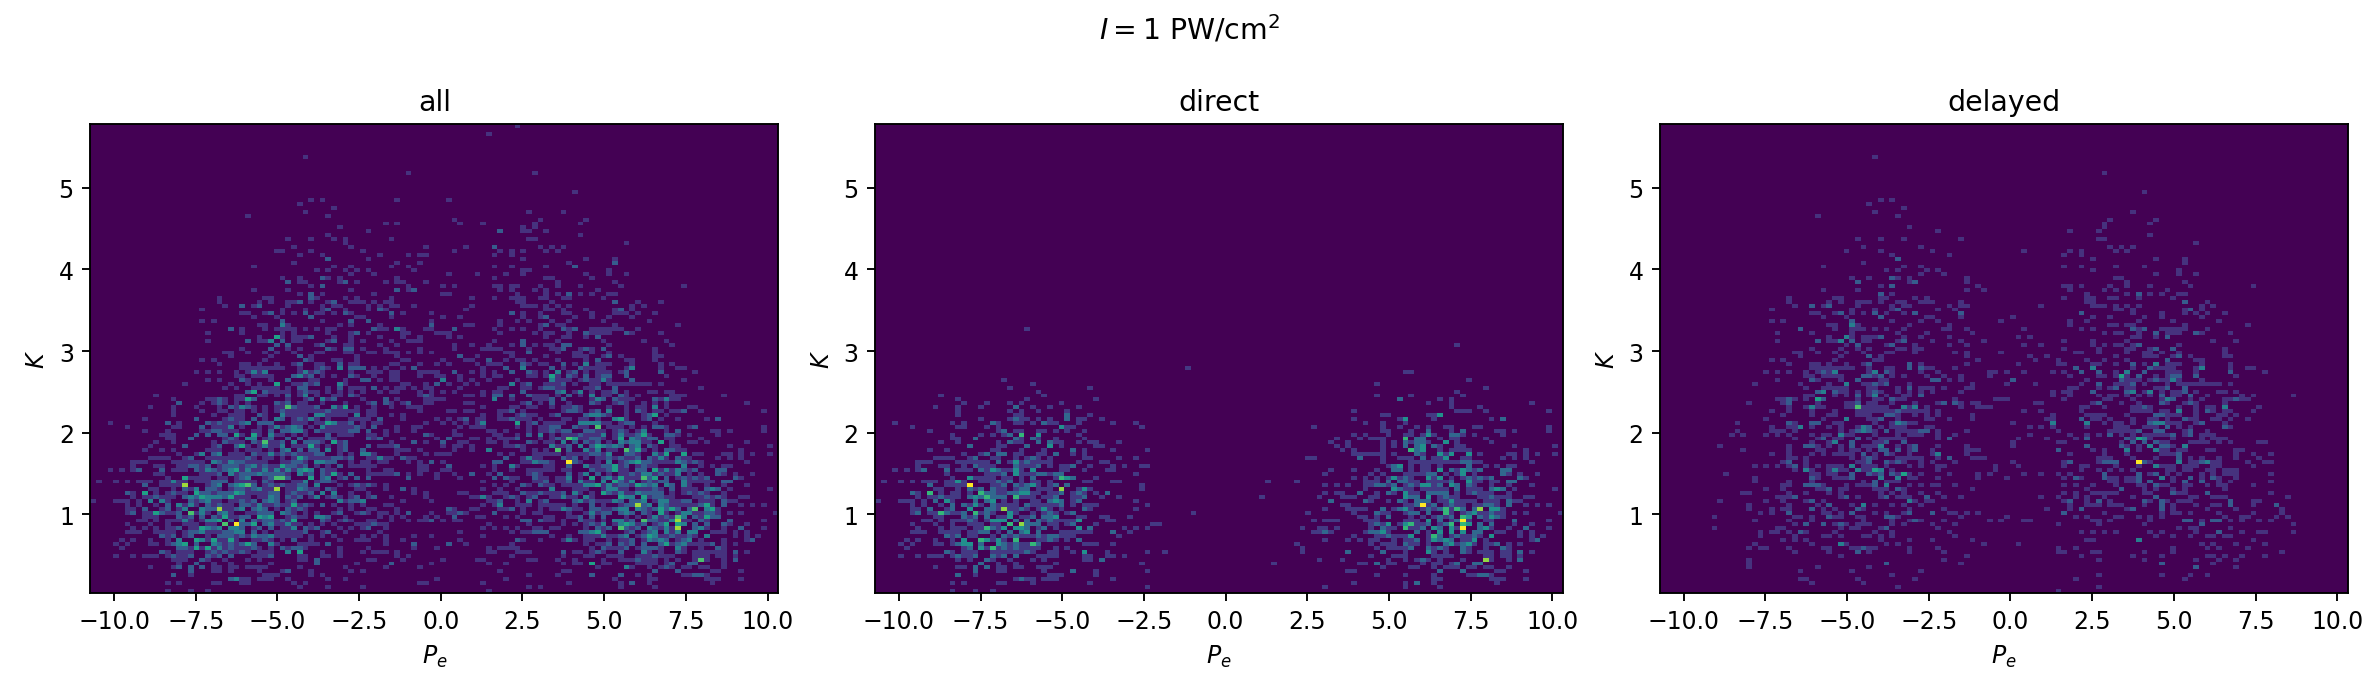
\includegraphics[width=0.95\textwidth]{P_vs_K_1p0.png}\\[-2pt]
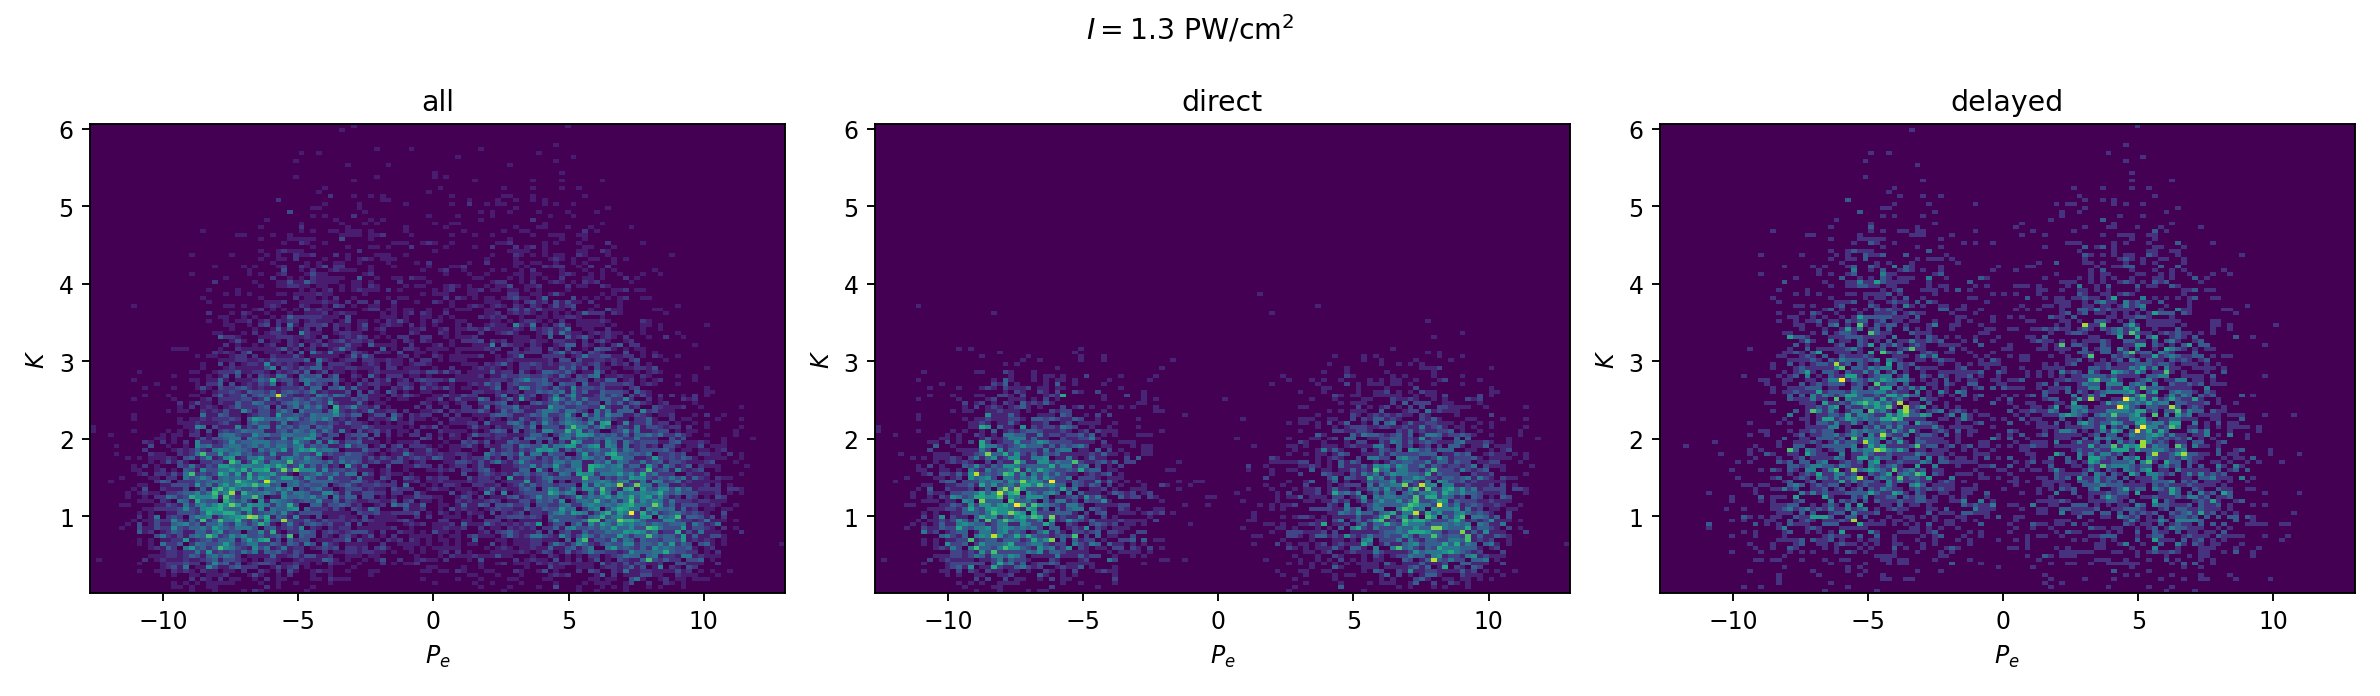
\includegraphics[width=0.95\textwidth]{P_vs_K_1p3.png}\\[-2pt]
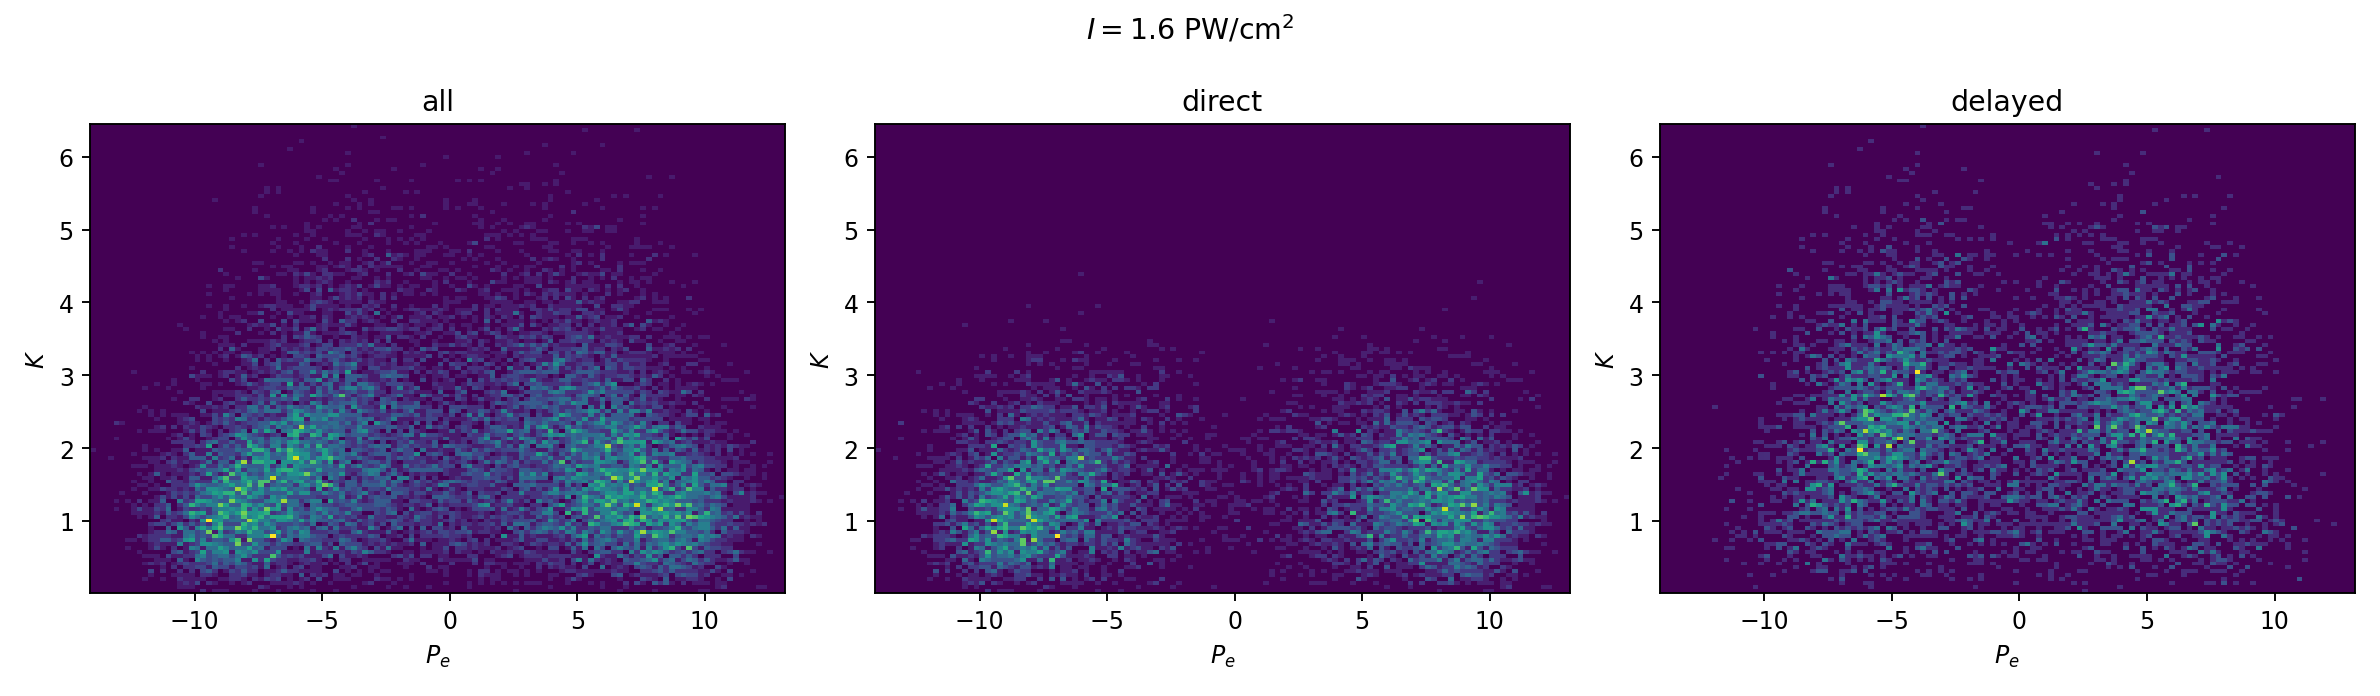
\includegraphics[width=0.95\textwidth]{P_vs_K_1p6.png}\\[-2pt]
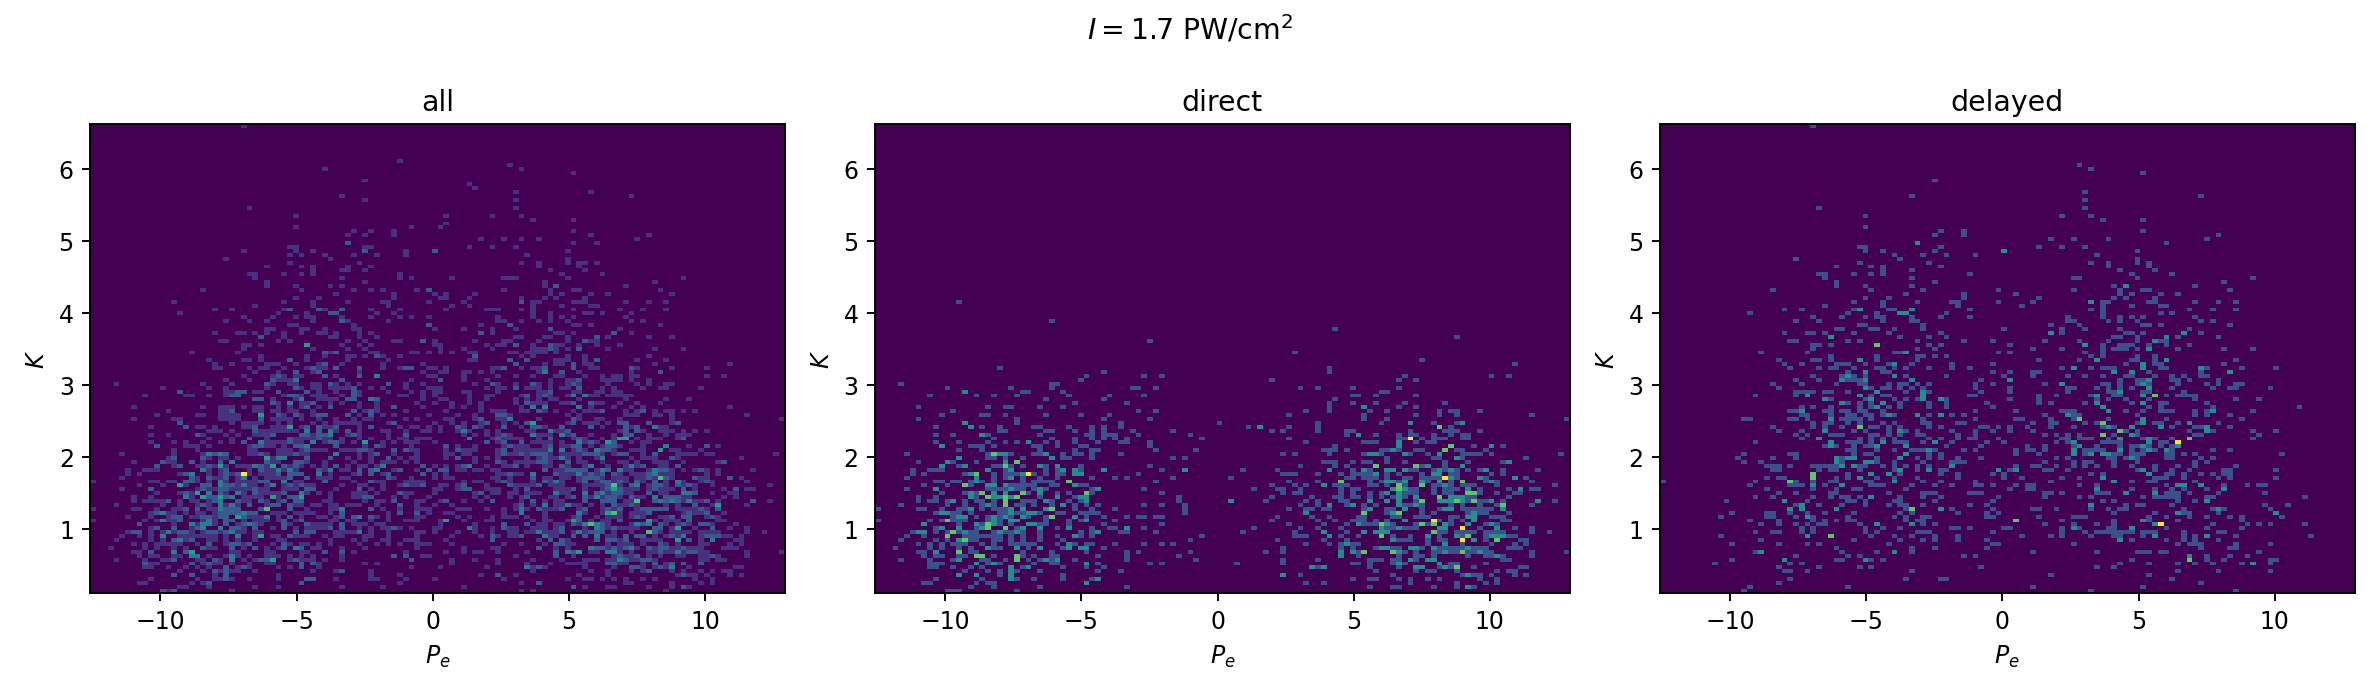
\includegraphics[width=0.95\textwidth]{P_vs_K_1p7.png}
\caption{Rozkład łączny sumy pędów podłużnych $P_e$ i skali
nierównowagi $K$. Kolejne wiersze odpowiadają intensywnościom
\num{1.0}, \num{1.3}, \num{1.6} i \num{1.7}~\PWcm, a w każdym wierszu
kolejne kolumny przedstawiają wszystkie zdarzenia, kanał \emph{direct}
i kanał \emph{delayed}.}
\label{fig:PeK}
\end{figure}

Inaczej mówiąc, rozkład \(P_e\) jest dwumodalny i
symetryczny względem zera, więc jego odchylenie standardowe
odzwierciedla przede wszystkim odstęp między maksimami, a nie ich
szerokość. Z tego powodu rozkład opisano dwiema osobnymi wielkościami.
Średnia wartość bezwzględna \(\langle|P_e|\rangle\) wyznacza
średnie położenie maksimów, a odchylenie standardowe \(|P_e|\) ich szerokość.
Obie wielkości zestawiono w tabeli~\ref{tab:glowna}.

Położenie maksimów wyraźnie zależy od kanału, ich wartości bezwzględne wynoszą od
\num{6.47} do \num{7.32}~\ja{} w kanale \emph{direct} oraz od
\num{4.32} do \num{4.96}~\ja{} w kanale \emph{delayed}. Szerokość
pojedynczego maksimum jest natomiast w obu kanałach zbliżona i mieści
się w przedziale od \num{1.58} do \num{2.42}~\ja{} Różnica między
kanałami dotyczy zatem głównie wartości bezwzględnej samych maksimów \(\langle|P_e|\rangle\), a nie szerokości tych rozkładów.

Wartość \(\langle|P_e|\rangle\) rośnie wraz z intensywnością pola,
ponieważ konsekwentnie wzrasta pęd dryfu (tabela~\ref{tab:impulsy}). Z tego względu zasadne jest obliczenie stosunku średniej wartości bezwzględnej sumy pędów
elektronów \(\langle|P_e|\rangle\) do pędu dryfu \(2\sqrt{U_p}\).
Otrzymana wielkość bezwymiarowa określa ile pędów dryfu zawarto w
średnim pędzie sumarycznym elektronów. Wyniki tego zestawienia zebrano
w tabeli~\ref{tab:dryf}.

\begin{table}[!h]
\centering
\caption{Średnia wartość bezwzględna sumy pędów podłużnych
$\langle|P_e|\rangle$ odniesiona do pędu dryfu $2\sqrt{U_p}$.}
\label{tab:dryf}
\begin{tabular}{c c c c c c}
\toprule
 &  & \multicolumn{2}{c}{\emph{direct}}
   & \multicolumn{2}{c}{\emph{delayed}} \\
\cmidrule(lr){3-4}
\cmidrule(lr){5-6}
$I$ [\PWcm] & $2\sqrt{U_p}$ [\ja] & $\langle|P_e|\rangle$ [\ja]
  & $\langle|P_e|\rangle/2\sqrt{U_p}$ & $\langle|P_e|\rangle$
  & $\langle|P_e|\rangle/2\sqrt{U_p}$ \\
\midrule
\num{1.0} & \num{2.964} & \num{6.466} & \num{2.181} & \num{4.320} & \num{1.457} \\
\num{1.3} & \num{3.379} & \num{7.064} & \num{2.091} & \num{4.799} & \num{1.420} \\
\num{1.6} & \num{3.749} & \num{7.316} & \num{1.952} & \num{4.961} & \num{1.323} \\
\num{1.7} & \num{3.671} & \num{7.165} & \num{1.952} & \num{4.856} & \num{1.323} \\
\bottomrule
\end{tabular}
\end{table}

Stosunek ten wyraźnie rozdziela oba kanały. W kanale \emph{direct}
maleje on od \num{2.18} do \num{1.95} wraz ze wzrostem intensywności, a w
kanale \emph{delayed} od \num{1.46} do \num{1.32}. Zakresy obu kanałów
są rozłączne, zatem różnica nie jest skutkiem samej skali pędu dryfu.
Zbiory \num{1.6} i \num{1.7}~\PWcm{} prowadzą do wartości zgodnych na
trzecim miejscu po przecinku, mimo odmiennych długości fali. Potwierdza to zależność wartości pędu dryfu od długości fali lasera.

\subsection{Płaszczyzna względna i skala nierównowagi}
\label{sec:wyn:K}

Następnie rozpatrzono ruch względny, opisany współrzędnymi
$(\xi_1,\xi_2)$ oraz skalą nierównowagi $K$~\eqref{eq:K}, mierzącą
odstępstwo od równego podziału pędu między elektronami.


\begin{figure}[!h]
\centering
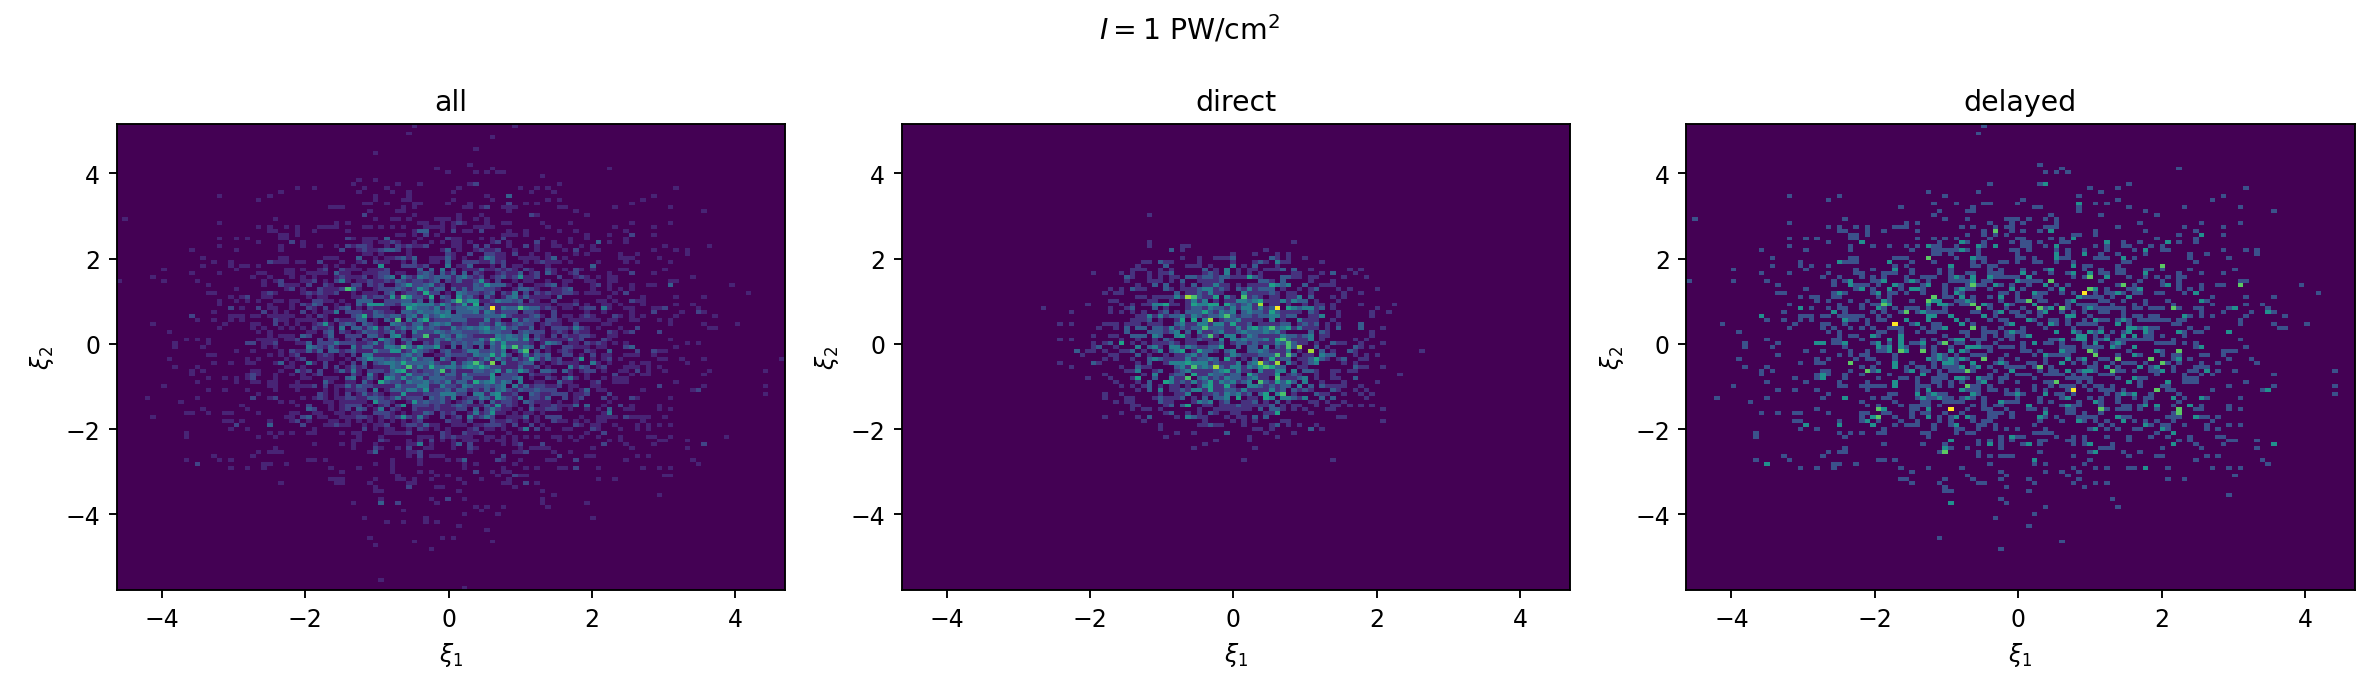
\includegraphics[width=0.95\textwidth]{relative_plane_1p0.png}\\[-2pt]
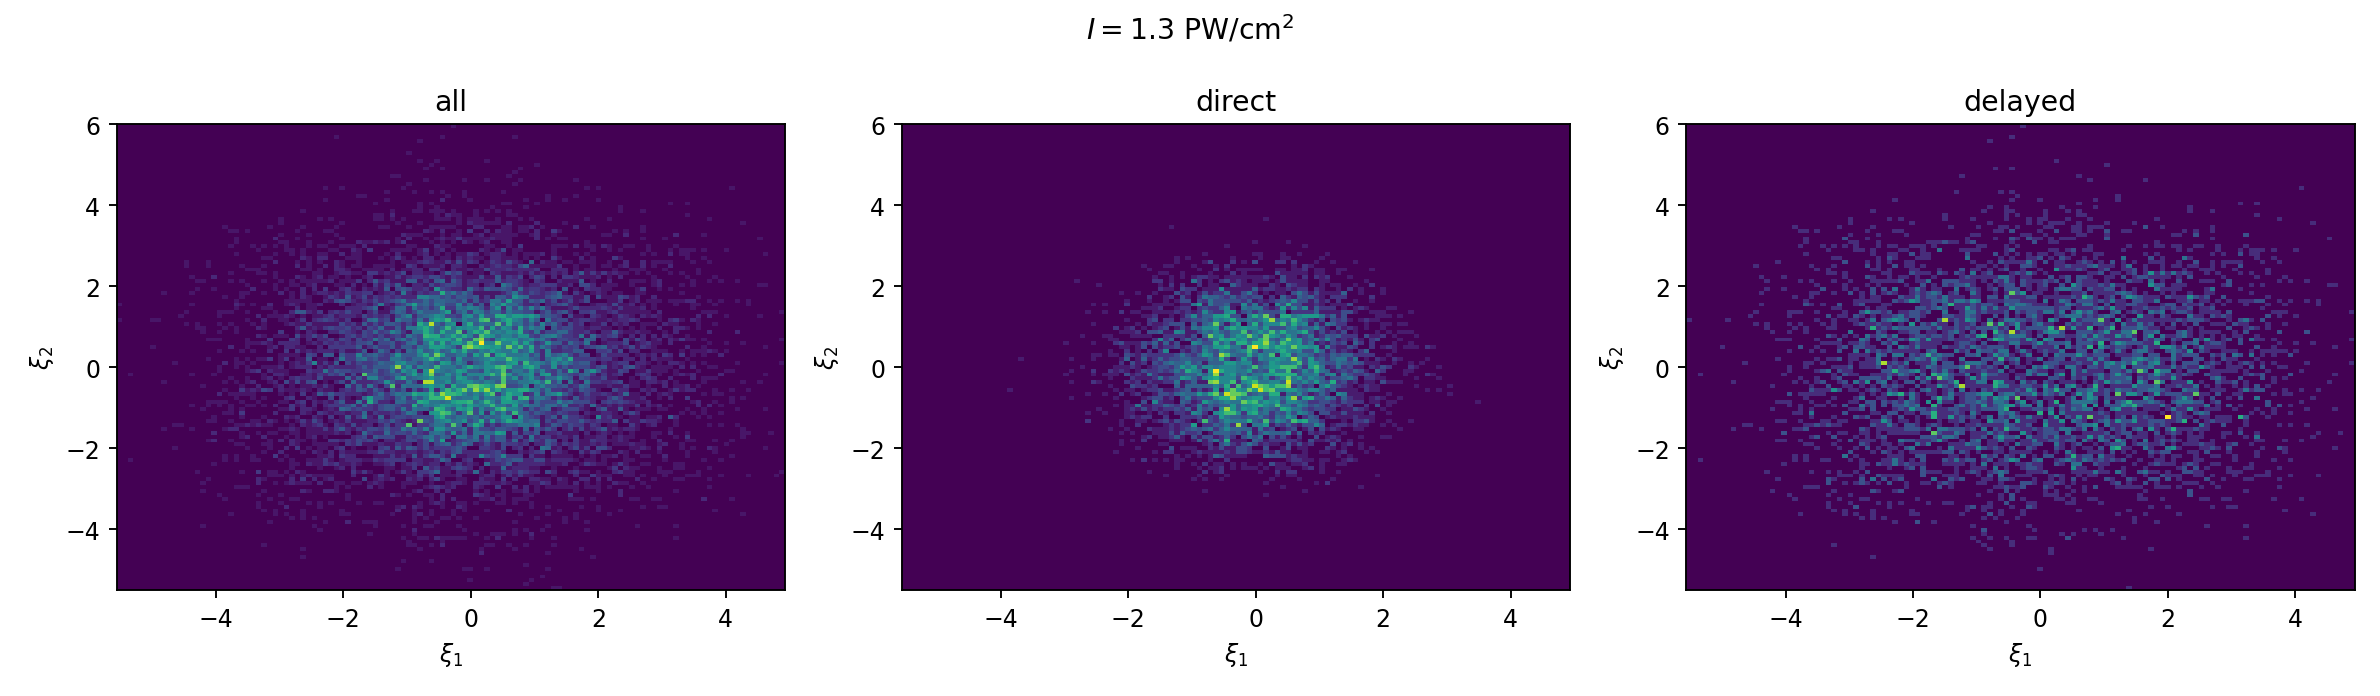
\includegraphics[width=0.95\textwidth]{relative_plane_1p3.png}\\[-2pt]
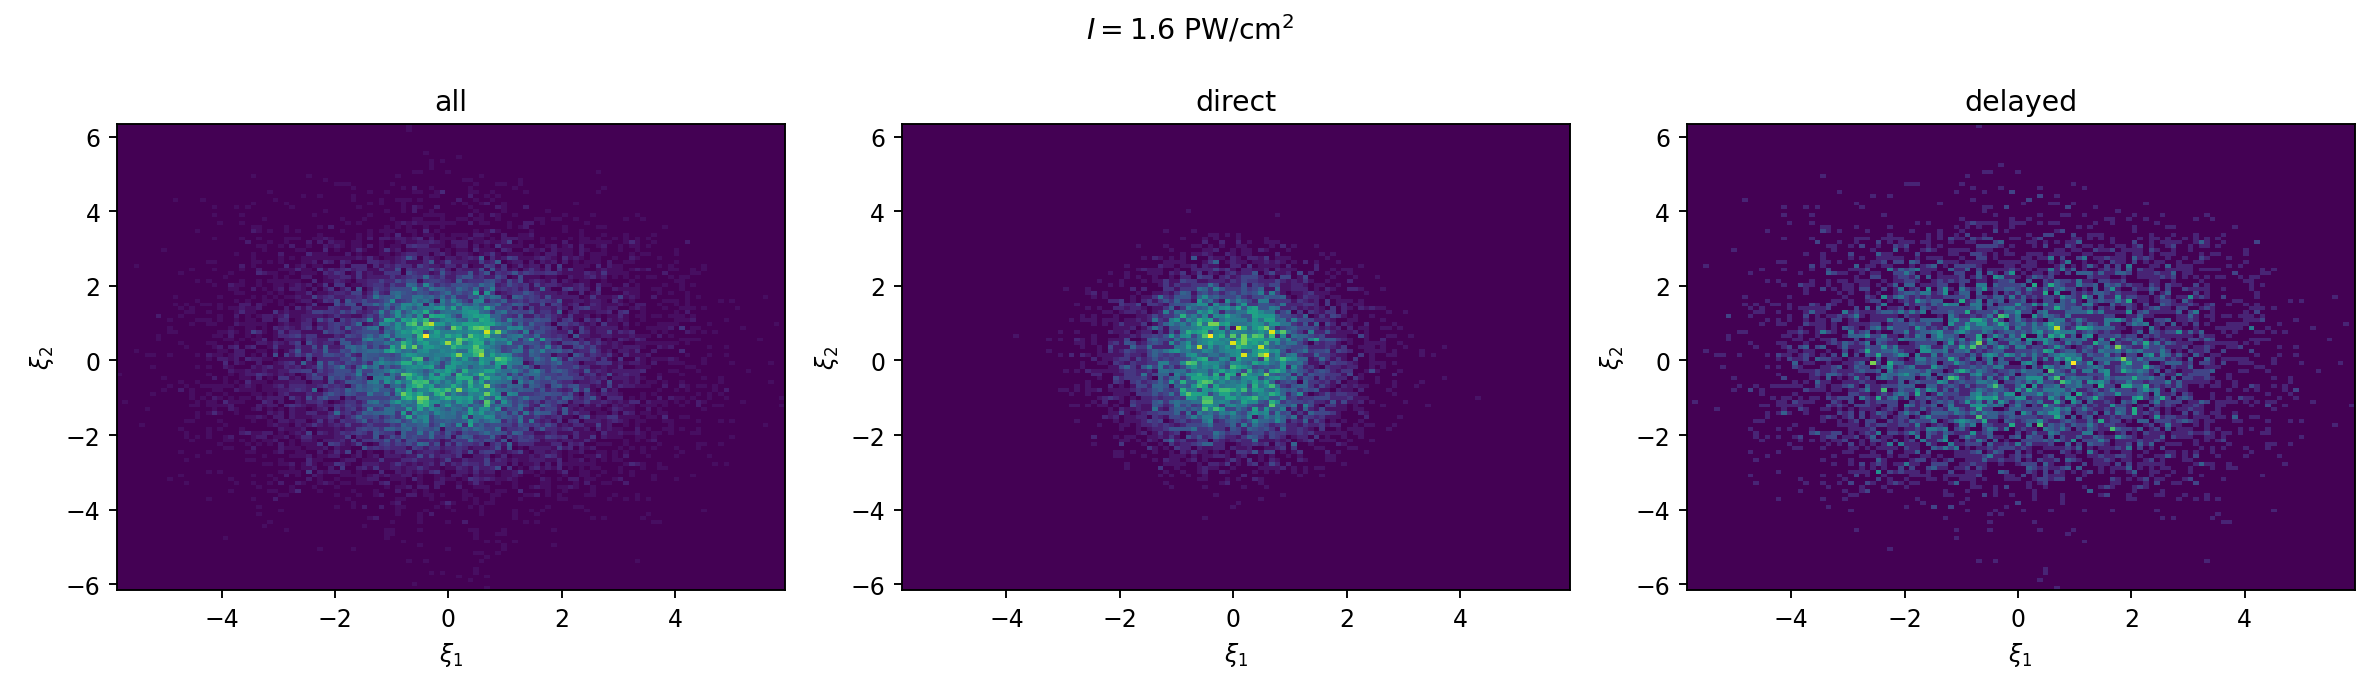
\includegraphics[width=0.95\textwidth]{relative_plane_1p6.png}\\[-2pt]
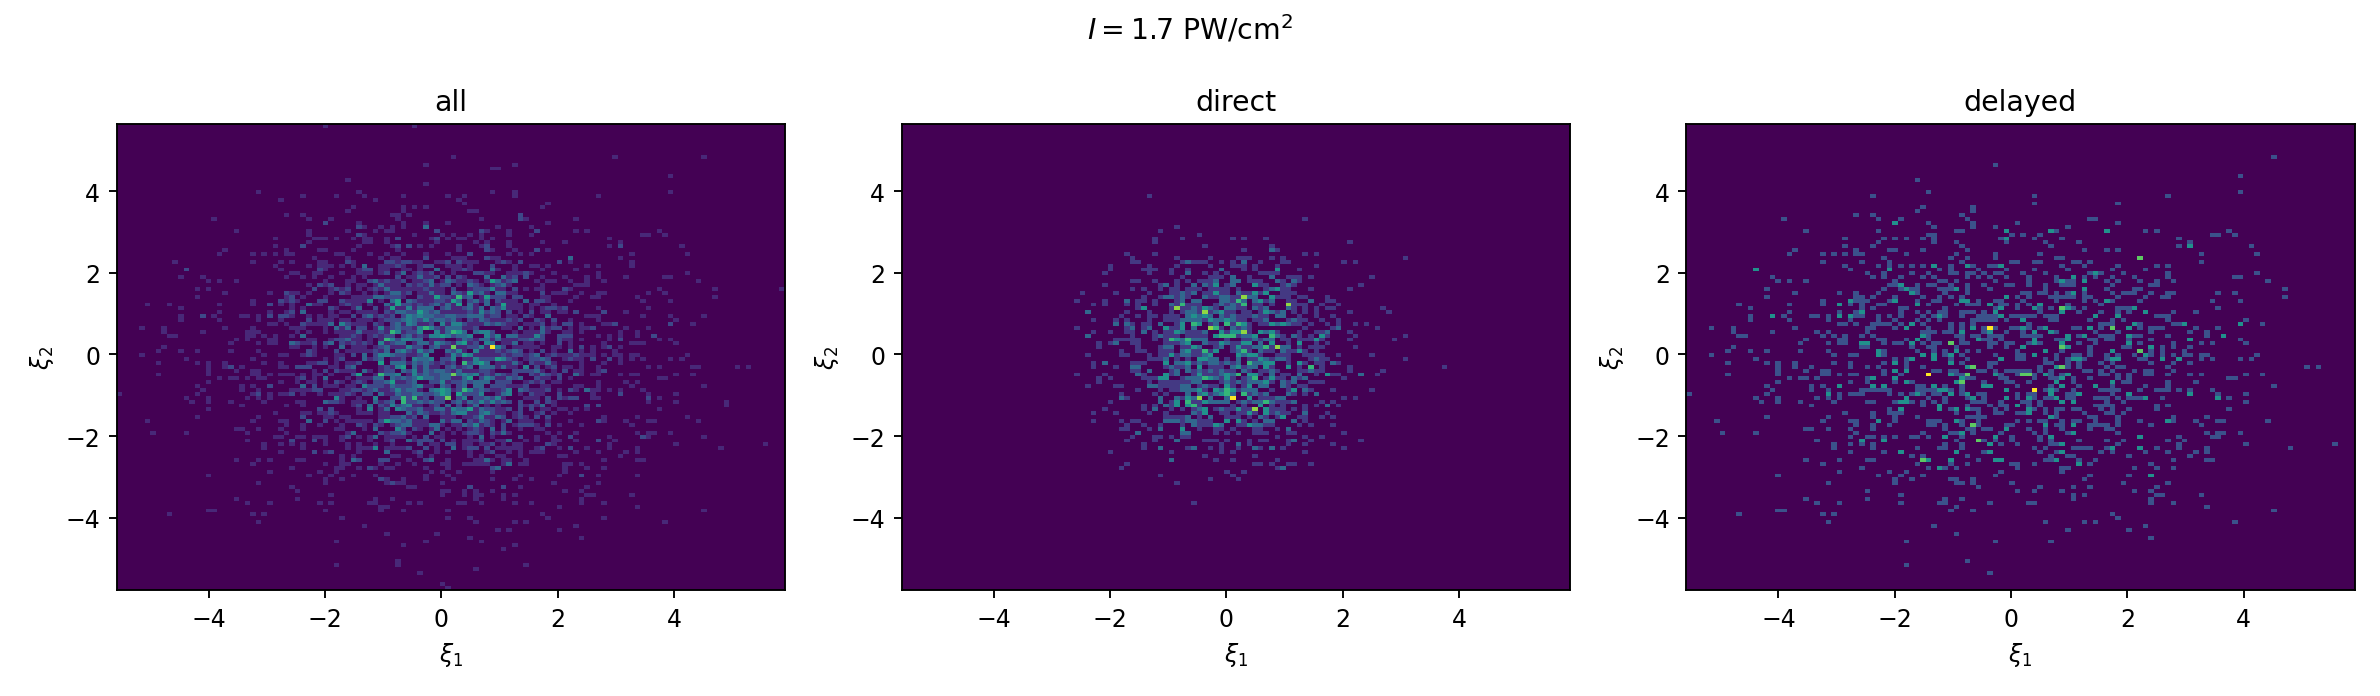
\includegraphics[width=0.95\textwidth]{relative_plane_1p7.png}
\caption{Rozkład na płaszczyźnie względnej $(\xi_1,\xi_2)$. Kolejne
wiersze odpowiadają intensywnościom \num{1.0}, \num{1.3}, \num{1.6} i
\num{1.7}~\PWcm, a układ kolumn jest taki sam jak na
rysunku~\ref{fig:PeK}. Współrzędna $\xi_1$ mierzy różnicę pędów
elektronów 2 i 3, a $\xi_2$ różnicę między parą 2--3 a elektronem 4.
Rozkłady o natężeniu pola $I =$ 1,7~\PWcm{} dotyczą innej długości fali.}
\label{fig:relplane}
\end{figure}

Na rysunku~\ref{fig:relplane} dla każdej z czterech intensywności rozkład dla kanału \emph{direct} jest
zwarty i skupiony wokół początku układu, natomiast dla kanału
\emph{delayed} jest wyraźnie szerszy. Potwierdzają to również wartości średnie
$\langle K\rangle$ zestawione w tabeli~\ref{tab:glowna}. Wartość bezwzględna różnicy między kanałami $| \langle K\rangle_{\mathrm{direct}}-\langle K\rangle_{\mathrm{delayed}}|$ leży około jedności, dokładne wartości zestawiono w tabeli~\ref{tab:welch}. 

Dla każdej z intensywności sprawdzono statystyczną istotność tej wartości za pomocą testu Welcha. Obliczono wartość $t$, określającą stosunek różnicy średnich wartości
skali nierównowagi do błędu standardowego tej różnicy, zgodnie ze wzorem:

\begin{equation}
  t=\frac{\langle K\rangle_{\mathrm{direct}}-\langle K\rangle_{\mathrm{delayed}}}
         {\sqrt{\dfrac{s_{\mathrm{direct}}^{2}}{n_{\mathrm{direct}}}
               +\dfrac{s_{\mathrm{delayed}}^{2}}{n_{\mathrm{delayed}}}}},
  \label{eq:welch}
\end{equation}

gdzie $s$ i $n$ oznaczają odpowiednio odchylenie standardowe średniej oraz liczbę zdarzeń
w kanale direct lub delayed. 

Przy założeniu hipotezy zerowej $H_0$ o równości średnich w obu
kanałach wielkość $t$ podlega rozkładowi $t$ Studenta, który przy tak
licznych próbkach został przybliżony za pomocą standardowego rozkładu normalnego. Dalej wyznaczono wartość $p$ jako pole pod krzywą tego rozkładu
poza przedziałem $(-|t|,|t|)$. Jest to prawdopodobieństwo otrzymania
różnicy co najmniej tak dużej jak zaobserwowana, gdyby $H_0$ była
prawdziwa. Otrzymane wartości $t$ i $p$ dla wszystkich intensywności zestawiono
w tabeli~\ref{tab:welch}.


\begin{table}[htbp]
  \centering
  \caption{Porównanie średniej skali nierównowagi $\langle K\rangle$
  w kanałach \emph{direct} i \emph{delayed} testem $t$ Welcha
  \eqref{eq:welch} dla wszystkich intensywności. $\Delta_{\langle K\rangle}=\langle K\rangle_{\mathrm{direct}}-\langle K\rangle_{\mathrm{delayed}}$
oznacza różnicę średnich.}
  \label{tab:welch}
  \begin{tabular}{cccccc}
    \toprule
    $I$ [\PWcm] & $\langle K\rangle_{\mathrm{direct}}$ [\ja]
      & $\langle K\rangle_{\mathrm{delayed}}$ [\ja] & $\Delta_{\langle K\rangle}$ [\ja]
      & $t$ & $p$ \\
    \midrule
    \num{1.0} & \num{1.182} & \num{2.121} & \num{-0.939} & \num{-40.0} & $<\num{1e-16}$ \\
    \num{1.3} & \num{1.295} & \num{2.276} & \num{-0.981} & \num{-63.0} & $<\num{1e-16}$ \\
    \num{1.6} & \num{1.417} & \num{2.337} & \num{-0.920} & \num{-62.7} & $<\num{1e-16}$ \\
    \num{1.7} & \num{1.398} & \num{2.383} & \num{-0.985} & \num{-30.1} & $<\num{1e-16}$ \\
    \bottomrule
  \end{tabular}
\end{table}

Przy każdej intensywności wartość $p$ jest mniejsza od \num{1e-16}. Hipotezę zerową o równości średnich odrzucono zatem we wszystkich
czterech przypadkach. Niższe wartości $|t|$ dla zbiorów \num{1.0}
i \num{1.7}~\PWcm{} wynikają z mniejszej liczby zdarzeń, ponieważ sama
różnica średnich jest tam porównywalna z pozostałymi.

Z drugiej strony, porównując rozkłady między kanałami, można zauważyć, że mają inny kształt. Wyznaczone odchylenia standardowe obu współrzędnych zestawiono
w tabeli~\ref{tab:sigmaxi}. W kanale \emph{direct} rozkład jest szerszy
wzdłuż $\xi_2$, a stosunek $\sigma(\xi_2)/\sigma(\xi_1)$ wynosi od
\num{1.16} do \num{1.25}. W kanale \emph{delayed} relacja jest odwrotna,
a stosunek wynosi od \num{0.84} do \num{0.94}. Ta sama zmiana relacji
występuje przy każdej intensywności.

\begin{table}[htbp]
  \centering
  \caption{Odchylenia standardowe współrzędnych względnych $\xi_1$
  i $\xi_2$ oraz ich stosunek w kanałach \emph{direct} i \emph{delayed}
  dla wszystkich intensywności. Odchylenia podano w~\ja}
  \label{tab:sigmaxi}
  \begin{tabular}{ccccccc}
    \toprule
    & \multicolumn{3}{c}{\emph{direct}} & \multicolumn{3}{c}{\emph{delayed}} \\
    \cmidrule(lr){2-4}\cmidrule(lr){5-7}
    $I$ [\PWcm] & $\sigma(\xi_1)$ & $\sigma(\xi_2)$ & $\sigma(\xi_2)/\sigma(\xi_1)$
                & $\sigma(\xi_1)$ & $\sigma(\xi_2)$ & $\sigma(\xi_2)/\sigma(\xi_1)$ \\
    \midrule
    \num{1.0} & \num{0.844} & \num{0.979} & \num{1.16} & \num{1.687} & \num{1.588} & \num{0.94} \\
    \num{1.3} & \num{0.926} & \num{1.097} & \num{1.18} & \num{1.862} & \num{1.663} & \num{0.89} \\
    \num{1.6} & \num{0.984} & \num{1.230} & \num{1.25} & \num{1.970} & \num{1.672} & \num{0.85} \\
    \num{1.7} & \num{0.972} & \num{1.205} & \num{1.24} & \num{2.014} & \num{1.699} & \num{0.84} \\
    \bottomrule
  \end{tabular}
\end{table}

Interpretacja wymaga ostrożności, ponieważ obie współrzędne
zdefiniowane są przez numery elektronów. Wynik oznacza, że w kanale
\emph{direct} największe różnice pędu występują między
parą elektronów początkowo związanych a elektronem
początkowo tunelującym, natomiast w kanale \emph{delayed}
wewnątrz pary elektronów początkowo związanych. Jest to
stwierdzenie o strukturze modelu, a nie o własności obserwowalnej.

Niezależnie od tego sprawdzono symetrię względem zamiany etykiet
elektronów 2 i 3. Elektrony te mają w modelu identyczny status elektronów początkowo związanych, więc
ich zamiana, odwracająca znak $\xi_1\rightarrow-\xi_1$, nie powinna
zmieniać rozkładu. Rozkład $\xi_1$ powinien być zatem symetryczny
względem zera, a średnie wartości pędów elektronów 2 i 3 $p_2$ i $p_3$ muszą być równe. 

Dla wszystkich
dwunastu zbiorów obliczono współczynniki skośności rozkładu $\xi_1$ zgodnie ze wzorem:

\begin{equation}
  \gamma_1=\frac{\dfrac{1}{n}\displaystyle\sum_{k=1}^{n}\left(\xi_{1,k}-\bar{\xi}_1\right)^{3}}
               {\left[\dfrac{1}{n}\displaystyle\sum_{k=1}^{n}\left(\xi_{1,k}-\bar{\xi}_1\right)^{2}\right]^{3/2}},
  \label{eq:skosnosc}
\end{equation}

gdzie $\xi_{1,k}$ oznacza wartość $\xi_1$ w $k$-tym zdarzeniu,
$\bar{\xi}_1$ jej średnią, a $n$ liczbę zdarzeń. Dla rozkładu
symetrycznego $\gamma_1=0$. Średnie $p_2$ i $p_3$ porównano testem
Welcha~\eqref{eq:welch}. Wyniki zestawiono w tabeli~\ref{tab:symetria}.

Współczynnik
skośności $\xi_1$ we wszystkich dwunastu zbiorach nie przekracza co do
modułu \num{0.056}. Dla średnich $p_2$ i $p_3$ w jedenastu z dwunastu zbiorów otrzymano $p$ od \num{0.43} do
\num{0.97}. Jedynie dla kanału \emph{delayed} przy \num{1.7}~\PWcm{}
wartość $p$ wynosi \num{0.034}. Przy dwunastu porównaniach prawdopodobieństwo
otrzymania co najmniej jednej takiej wartości odstającej przy prawdziwej $H_0$
wynosi około \num{0.46}. Dlatego zastosowano poprawkę Bonferroniego~\cite{Dunn1961}, zgodnie
z którą każdą wartość $p$ porównuje się z progiem
$\num{0.05}/12\approx\num{0.0042}$. Jeżeli wartość $p$ jest większa niż ten
próg, nie ma podstaw do odrzucenia hipotezy zerowej $H_0$ o równości
średnich $p_2$ i $p_3$. Żadna z otrzymanych wartości nie jest mniejsza od progu, więc dane są zgodne z symetrią względem zamiany elektronów 2 i 3.

\begin{table}[htbp]
  \centering
  \caption{Sprawdzenie symetrii względem zamiany elektronów 2 i 3.
  Podano współczynnik skośności $\gamma_1$ rozkładu $\xi_1$
  \eqref{eq:skosnosc}, średnie wartości $p_2$ i $p_3$ wraz
  z odchyleniem standardowym średniej $s/\sqrt{n}$ oraz wynik testu
  Welcha ich równości.}
  \label{tab:symetria}
  \begin{tabular}{llccccc}
    \toprule
    $I$ [\PWcm] & kanał & $\gamma_1(\xi_1)$ & $\langle p_2\rangle$ [\ja]
      & $\langle p_3\rangle$ [\ja] & $t$ & $p$ \\
    \midrule
    \num{1.0} & \emph{direct}  & \num{-0.052} & $\num{-0.009}\pm\num{0.051}$ & $\num{-0.019}\pm\num{0.051}$ & \num{0.13}  & \num{0.89} \\
              & \emph{delayed} & \num{-0.001} & $\num{-0.047}\pm\num{0.043}$ & $\num{0.001}\pm\num{0.043}$  & \num{-0.80} & \num{0.43} \\
              & wszystkie      & \num{-0.018} & $\num{-0.014}\pm\num{0.030}$ & $\num{-0.006}\pm\num{0.029}$ & \num{-0.19} & \num{0.85} \\
    \midrule
    \num{1.3} & \emph{direct}  & \num{-0.054} & $\num{-0.050}\pm\num{0.033}$ & $\num{-0.036}\pm\num{0.033}$ & \num{-0.30} & \num{0.76} \\
              & \emph{delayed} & \num{-0.014} & $\num{0.007}\pm\num{0.028}$  & $\num{0.025}\pm\num{0.029}$  & \num{-0.46} & \num{0.65} \\
              & wszystkie      & \num{-0.034} & $\num{-0.019}\pm\num{0.020}$ & $\num{-0.001}\pm\num{0.020}$ & \num{-0.63} & \num{0.53} \\
    \midrule
    \num{1.6} & \emph{direct}  & \num{0.053}  & $\num{-0.015}\pm\num{0.029}$ & $\num{-0.017}\pm\num{0.029}$ & \num{0.04}  & \num{0.97} \\
              & \emph{delayed} & \num{-0.009} & $\num{-0.009}\pm\num{0.027}$ & $\num{-0.006}\pm\num{0.026}$ & \num{-0.09} & \num{0.93} \\
              & wszystkie      & \num{-0.011} & $\num{-0.005}\pm\num{0.018}$ & $\num{-0.012}\pm\num{0.018}$ & \num{0.28}  & \num{0.78} \\
    \midrule
    \num{1.7} & \emph{direct}  & \num{0.056}  & $\num{0.132}\pm\num{0.065}$  & $\num{0.092}\pm\num{0.065}$  & \num{0.43}  & \num{0.67} \\
              & \emph{delayed} & \num{0.010}  & $\num{-0.094}\pm\num{0.057}$ & $\num{0.076}\pm\num{0.057}$  & \num{-2.12} & \num{0.034} \\
              & wszystkie      & \num{-0.037} & $\num{0.013}\pm\num{0.039}$  & $\num{0.053}\pm\num{0.039}$  & \num{-0.72} & \num{0.47} \\
    \bottomrule
  \end{tabular}
\end{table}

\subsection{Podział pędu bezwzględnego}
\label{sec:wyn:Neff}

Wielkość $K$ zależy od skali pędów, dlatego sam podział
pędu opisano obserwablami bezwymiarowymi z
podrozdziału~\ref{sec:obserwable}.

\begin{figure}[!h]
\centering
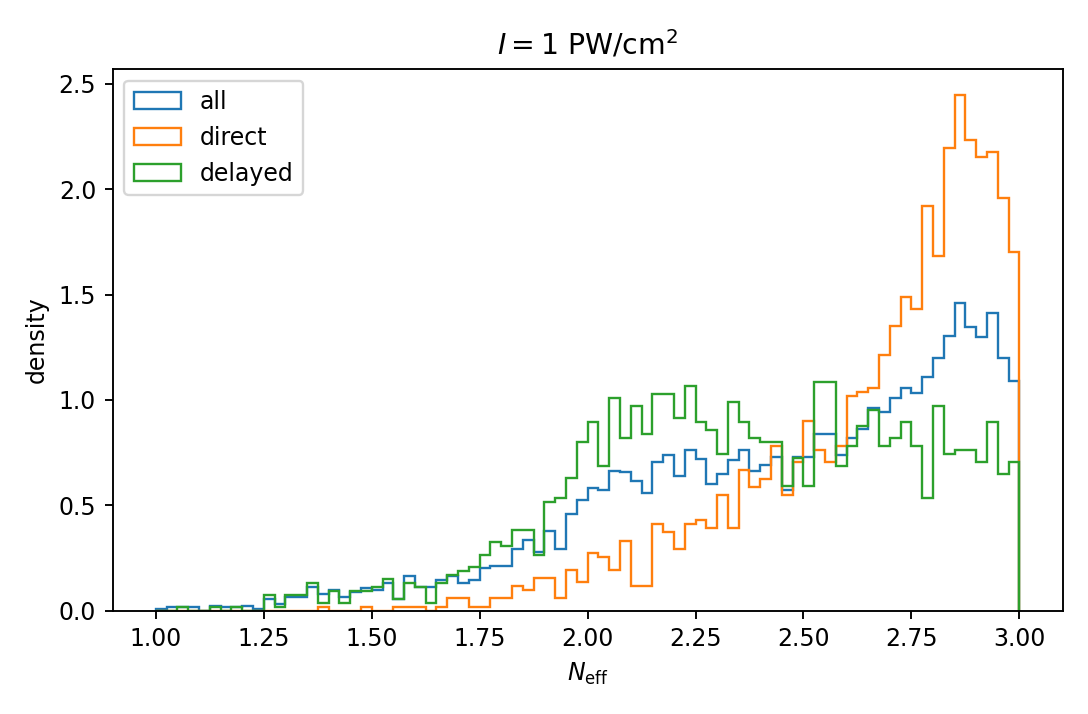
\includegraphics[width=0.49\textwidth]{Neff_1p0.png}
\hfill
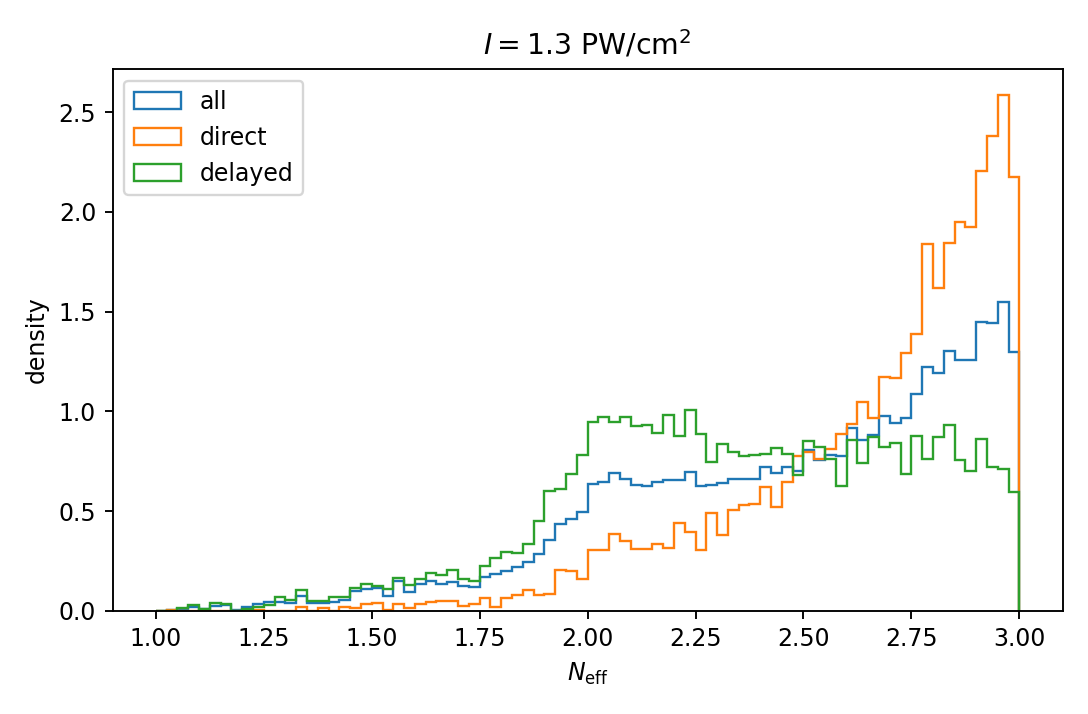
\includegraphics[width=0.49\textwidth]{Neff_1p3.png}\\[4pt]
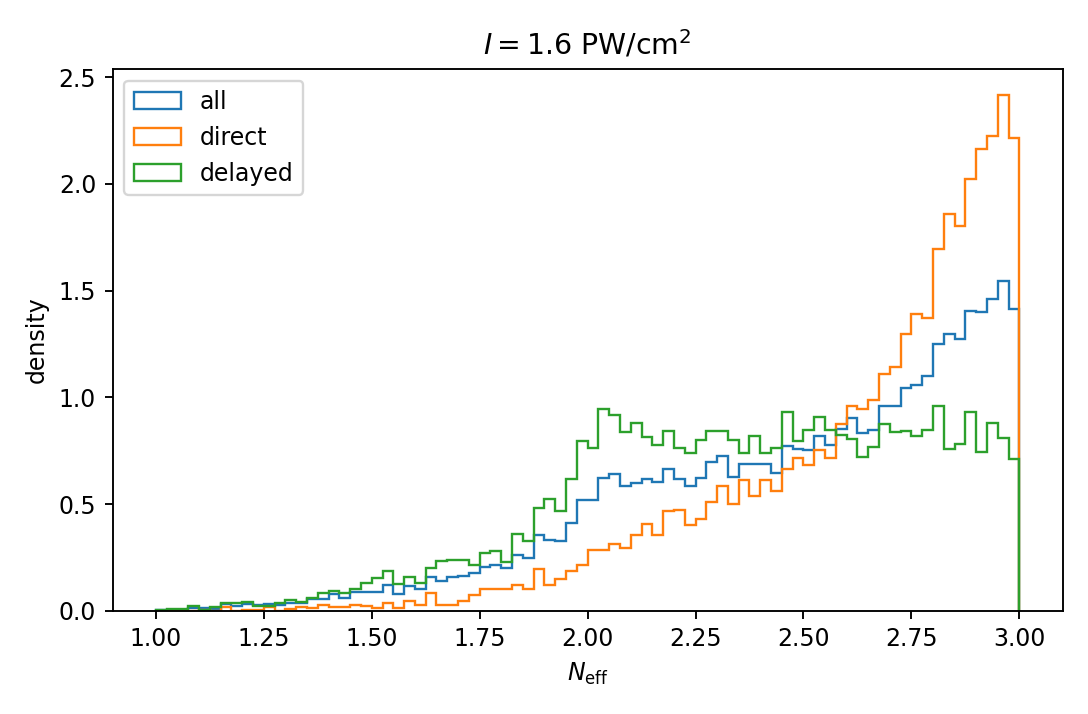
\includegraphics[width=0.49\textwidth]{Neff_1p6.png}
\hfill
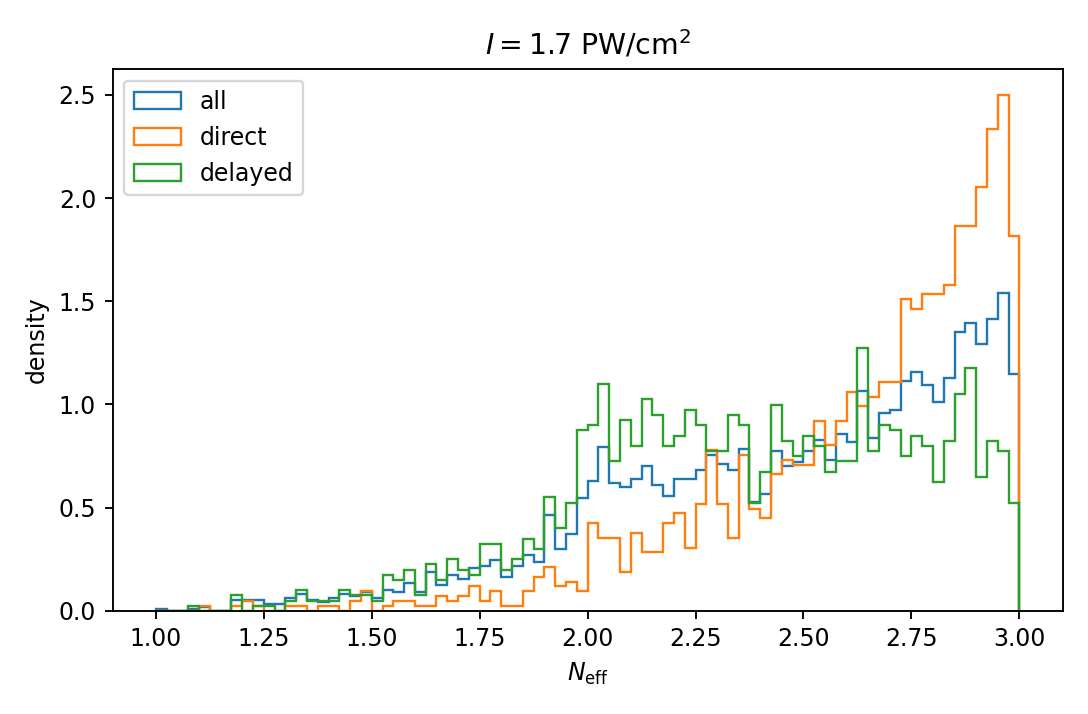
\includegraphics[width=0.49\textwidth]{Neff_1p7.png}
\caption{Rozkład efektywnej liczby elektronów $\Neff$. W górnym wierszu
\num{1.0} i \num{1.3}~\PWcm, w dolnym \num{1.6} i \num{1.7}~\PWcm.
Wartość $\Neff=3$ odpowiada równemu podziałowi pędu między trzy
elektrony, $\Neff=2$ podziałowi między dwa elektrony przy trzecim
niosącym znikomy pęd. Zbiór \num{1.7}~\PWcm{} policzono dla innej
długości fali.}
\label{fig:neff}
\end{figure}

Rozkłady efektywnej liczby elektronów $\Neff$ na rysunku~\ref{fig:neff} dla różnych kanałów wyglądają inaczej, przy czym różnica ta ma tę samą postać przy każdej z czterech intensywności. W kanale \emph{direct} występuje jedno wyraźne maksimum tuż przy
$\Neff=3$. W kanale \emph{delayed} rozkład jest bardziej płaski, z szerokim maksimum w okolicach $\Neff\approx\num{2.1}$ i wyraźnym drugim
obszarem podwyższonej gęstości przy $\Neff\approx\num{2.8}$. Rozkład dla
wszystkich zdarzeń leży pomiędzy nimi, co jest oczekiwane, ponieważ
zawiera oba kanały.

Wartości średnie $\langle\Neff\rangle$ zebrano w tabeli~\ref{tab:glowna}.
Przy każdej intensywności $\langle\Neff\rangle$ jest większa w kanale
\emph{direct} niż w kanale \emph{delayed}, a różnica wynosi od
\num{0.254} do \num{0.299}. Różnica ta jest istotna statystycznie w każdym z czterech przypadków,
co sprawdzono testem Welcha~\eqref{eq:welch} w ten sam sposób jak dla
skali nierównowagi $K$. Otrzymane wartości $t$ i $p$ zebrano
w tabeli~\ref{tab:welch_neff}. Wartość $t$ w teście Welcha wynosi od
\num{20.5} do \num{46.9}, a $p<\num{1e-16}$. Przedziały ufności obu
kanałów nie zachodzą na siebie.

\begin{table}[htbp]
  \centering
  \caption{Porównanie średniej efektywnej liczby elektronów
  $\langle\Neff\rangle$ w kanałach \emph{direct} i \emph{delayed}
  testem $t$ Welcha dla wszystkich intensywności.
  $\Delta_{\langle\Neff\rangle}=\langle\Neff\rangle_{\mathrm{direct}}-\langle\Neff\rangle_{\mathrm{delayed}}$
  oznacza różnicę średnich.}
  \label{tab:welch_neff}
  \begin{tabular}{cccccc}
    \toprule
    $I$ [\PWcm] & $\langle\Neff\rangle_{\mathrm{direct}}$
      & $\langle\Neff\rangle_{\mathrm{delayed}}$
      & $\Delta_{\langle\Neff\rangle}$ & $t$ & $p$ \\
    \midrule
    \num{1.0} & \num{2.662} & \num{2.367} & \num{0.294} & \num{28.4} & $<\num{1e-16}$ \\
    \num{1.3} & \num{2.654} & \num{2.355} & \num{0.299} & \num{46.9} & $<\num{1e-16}$ \\
    \num{1.6} & \num{2.633} & \num{2.367} & \num{0.266} & \num{46.7} & $<\num{1e-16}$ \\
    \num{1.7} & \num{2.628} & \num{2.374} & \num{0.254} & \num{20.5} & $<\num{1e-16}$ \\
    \bottomrule
  \end{tabular}
\end{table}

We wszystkich dwunastu zbiorach $\langle\Neff\rangle$ leży powyżej
odniesienia \num{2.118} odpowiadającego rozkładowi bez żadnej
preferencji. Analogicznie $\langle\xmax\rangle$ mieści się w przedziale
od \num{0.464} do \num{0.473} dla kanału \emph{direct} i od \num{0.530}
do \num{0.536} dla kanału \emph{delayed}, a więc w obu przypadkach
istotnie poniżej odniesienia \num{0.611}.


Wnioskując z otrzymanych wartości, w obu kanałach podział pędu jest bardziej równomierny, niż wynikałoby to z przypadku, a w kanale
\emph{direct} jest wyraźnie bardziej równomierny niż w kanale
\emph{delayed}, sądząc po statystycznie mniejszych wartościach $\langle\xmax\rangle$. Jest to zgodne z sensem fizycznym obu ścieżek, w kanale
\emph{direct} wszystkie trzy elektrony uzyskują energię w jednym
zderzeniu i opuszczają atom w podobny sposób, natomiast w kanale
\emph{delayed} trzeci elektron jonizuje się później i robi to niezależnie, co skutkuje bardziej nierównym podziałem pędu i większą wartością $\langle\xmax\rangle$.

\subsection{Sektory znakowe}
\label{sec:wyn:sektory}

\begin{figure}[H]
\centering
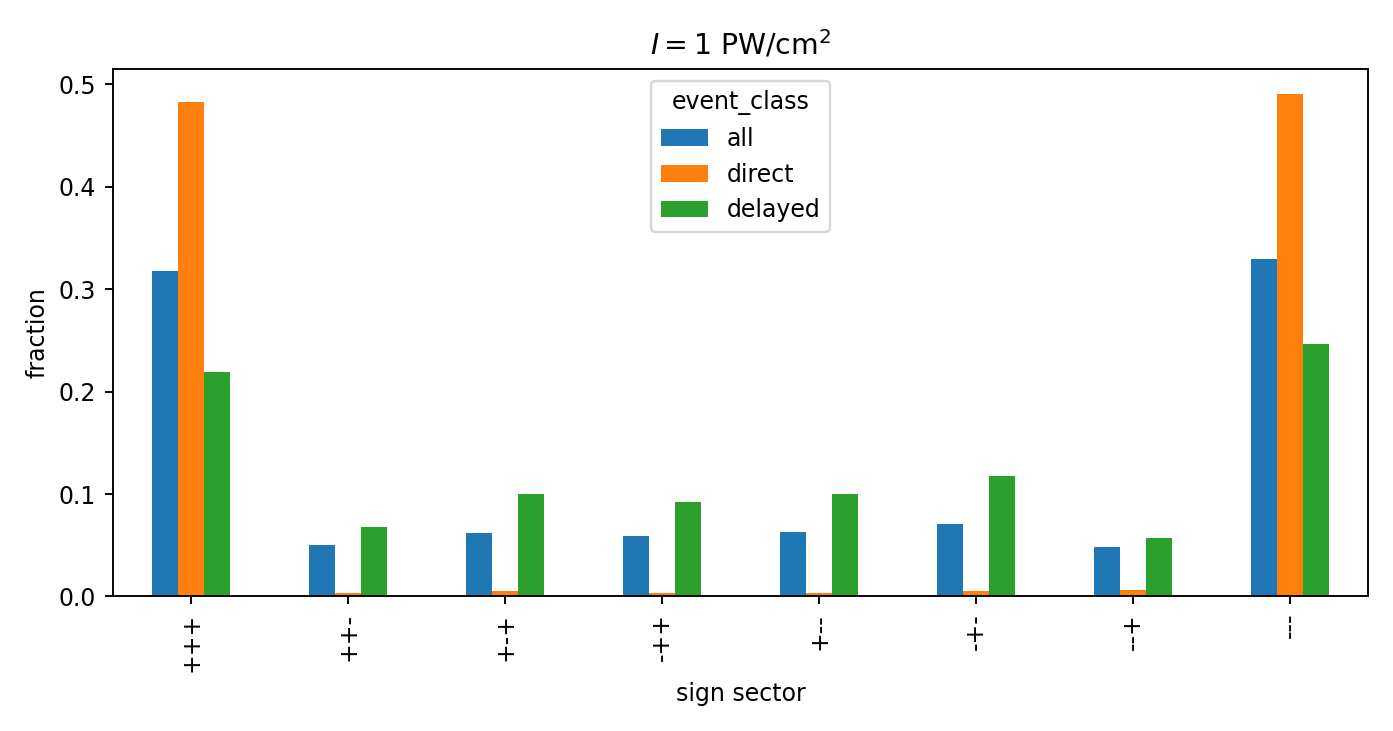
\includegraphics[width=0.49\textwidth]{sign_sectors_1p0.png}
\hfill
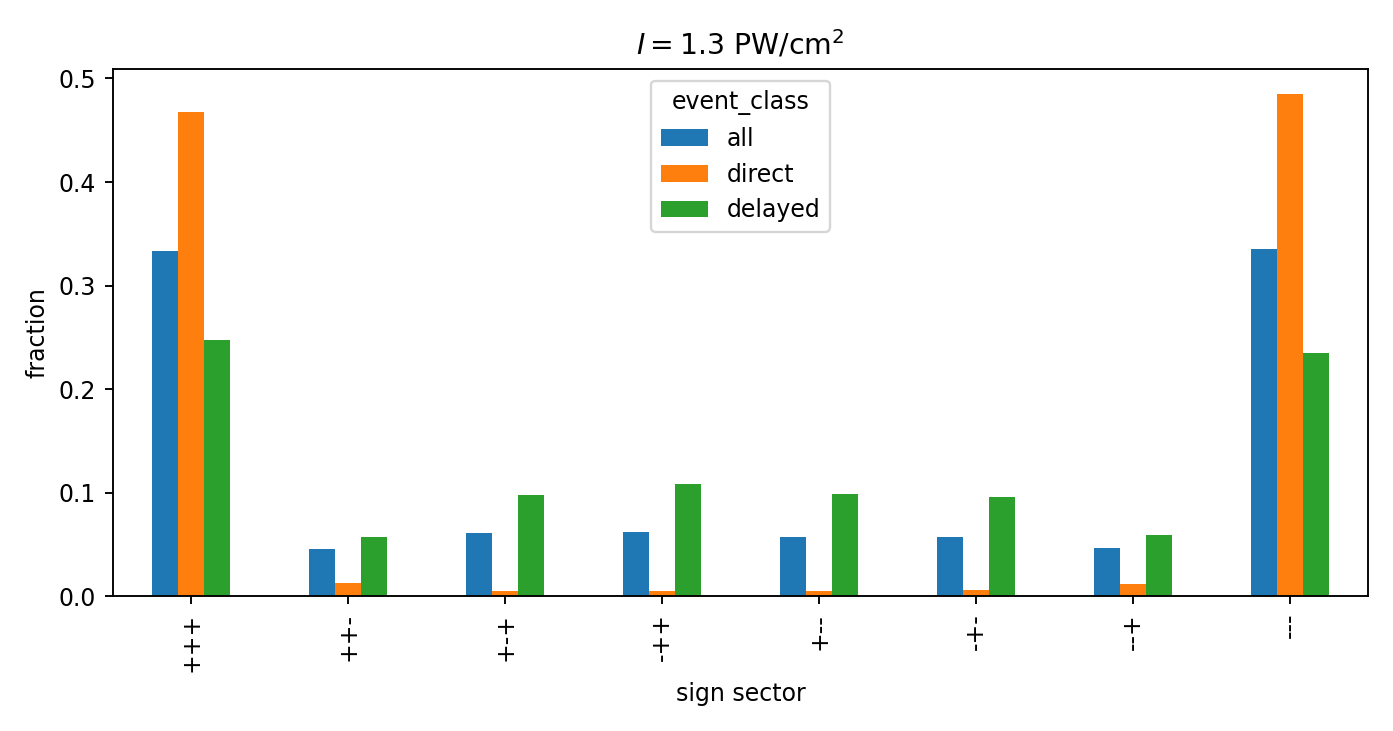
\includegraphics[width=0.49\textwidth]{sign_sectors_1p3.png}\\[4pt]
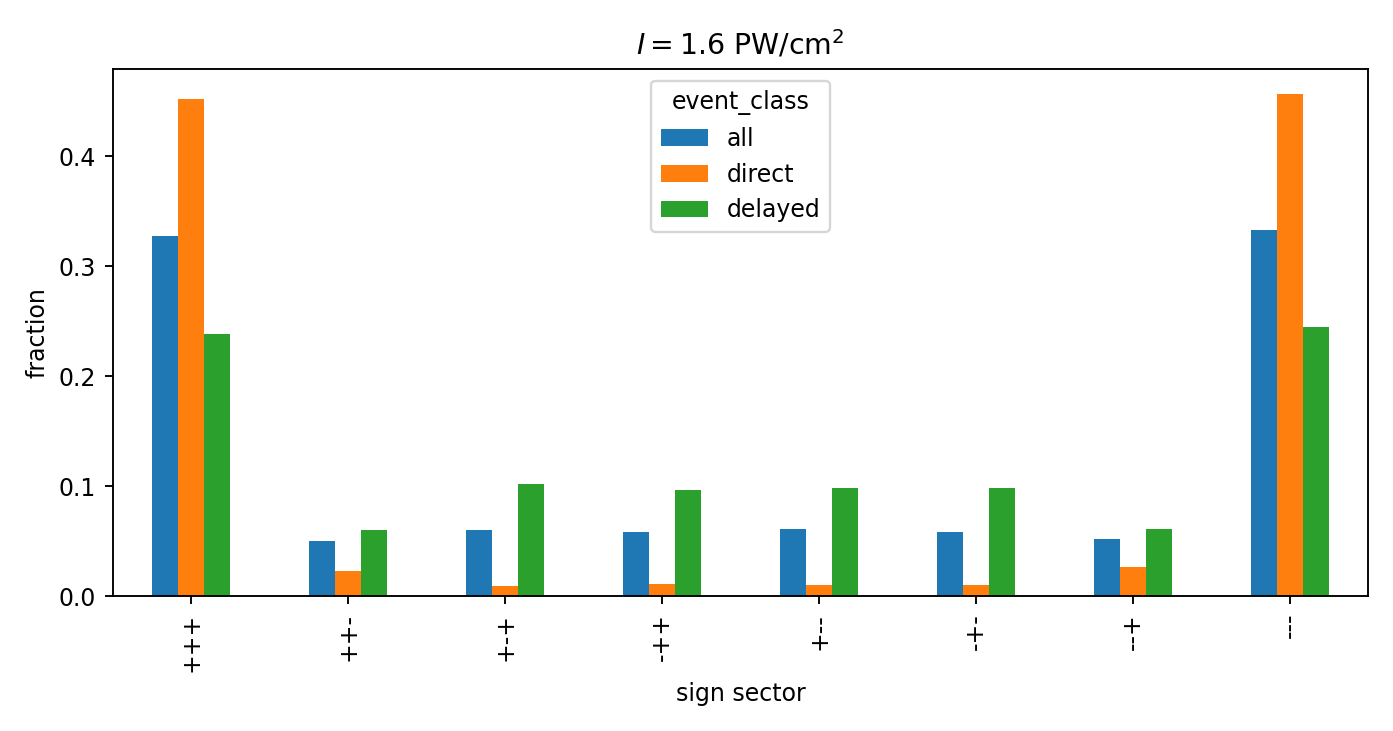
\includegraphics[width=0.49\textwidth]{sign_sectors_1p6.png}
\hfill
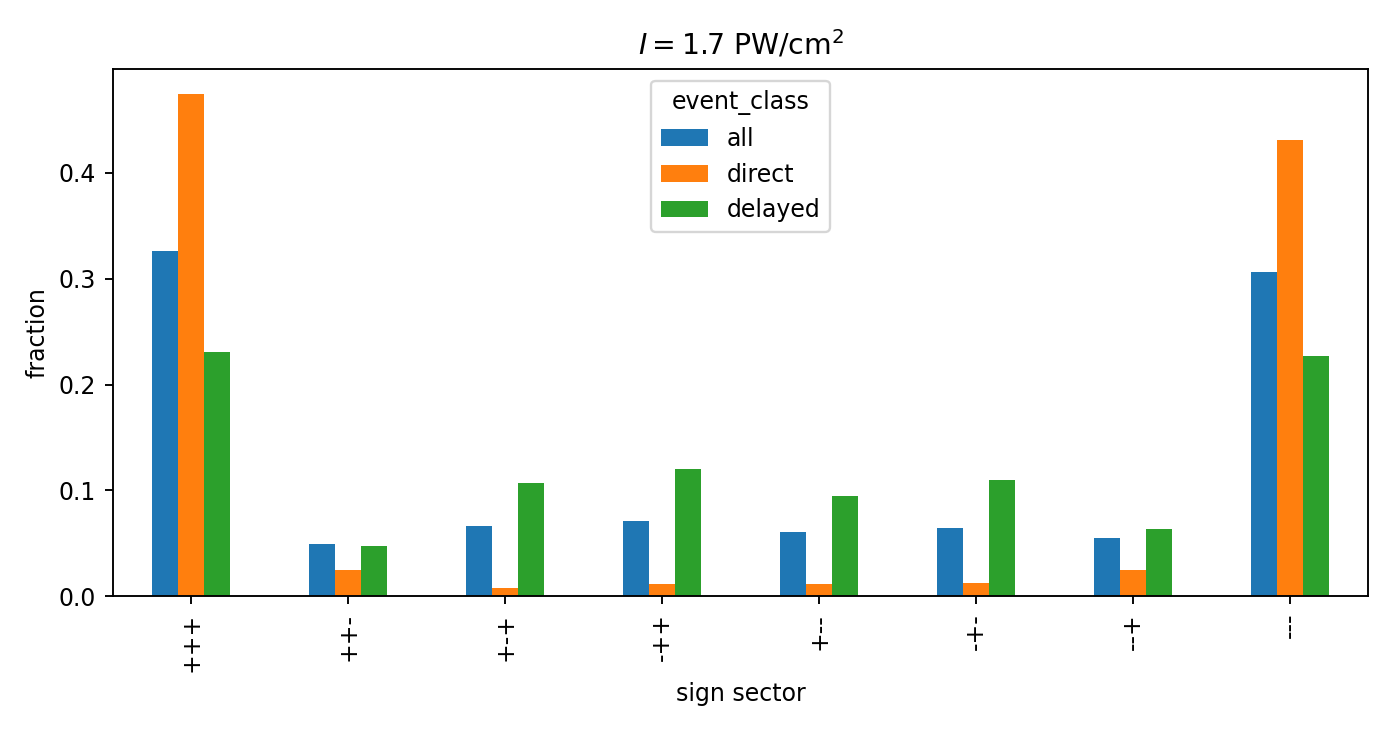
\includegraphics[width=0.49\textwidth]{sign_sectors_1p7.png}
\caption{Udział poszczególnych sektorów znakowych trójki
$(p_2,p_3,p_4)$. W górnym wierszu \num{1.0} i \num{1.3}~\PWcm,
w dolnym \num{1.6} i \num{1.7}~\PWcm. Sektory \texttt{+++} i \texttt{---}
odpowiadają emisji wszystkich elektronów w tę samą stronę. Zbiór
\num{1.7}~\PWcm{} policzono dla innej długości fali.}
\label{fig:sektory}
\end{figure}

Rysunek~\ref{fig:sektory} pokazuje wyraźną różnicę między
kanałami, taką samą przy każdej z czterech intensywności. W kanale
\emph{direct} niemal wszystkie zdarzenia leżą w dwóch sektorach
zgodnych, a sześć sektorów mieszanych jest prawie pustych. W kanale
\emph{delayed} dwa sektory o kierunku zgodnym pozostają najliczniejsze, ale
sektory mieszane są wyraźnie obsadzone i mają zbliżone udziały.

Udział zdarzeń, w których wszystkie elektrony poruszają się w tę samą stronę, $f_{\mathrm{zg}}$ zestawiono
w tabeli~\ref{tab:fzg}. We wszystkich dwunastu zbiorach znacznie
przewyższa on odniesienie \num{0.25} dla znaków niezależnych, co
potwierdza, że emisja jest skorelowana. W kanale \emph{direct}
$f_{\mathrm{zg}}$ wynosi od \num{0.905} do \num{0.974}, a w kanale
\emph{delayed} od \num{0.457} do \num{0.483}. Wielkość $f_{\mathrm{zg}}$
jest średnią zmiennej przyjmującej wartość 1 dla zdarzenia z sektora
zgodnego i 0 dla zdarzenia z sektora mieszanego. Różnicę między
kanałami sprawdzono więc tym samym testem Welcha~\eqref{eq:welch},
przyjmując za $s^2$ wariancję tej zmiennej
$f_{\mathrm{zg}}(1-f_{\mathrm{zg}})$. Wartość $t$ wynosi od \num{31.2}
do \num{66.5}, a $p<\num{1e-16}$ przy każdej intensywności. Jedyną
zauważalną zależnością w serii \num{800}~nm jest stopniowy spadek
$f_{\mathrm{zg}}$ w kanale \emph{direct} wraz ze wzrostem natężenia
pola, omówiony bardziej szczegółowo w podrozdziale~\ref{sec:wyn:intensywnosc}.

\begin{table}[htbp]
  \centering
  \caption{Udział emisji w tę samą stronę $f_{\mathrm{zg}}$, czyli
  zdarzeń o znakach $(+{+}+)$ lub $(-{-}-)$, oraz porównanie kanałów
  testem Welcha.
  $\Delta_{f}=f_{\mathrm{zg}}^{\mathrm{direct}}-f_{\mathrm{zg}}^{\mathrm{delayed}}$
  oznacza różnicę udziałów. Dla znaków niezależnych
  $f_{\mathrm{zg}}=\num{0.25}$.}
  \label{tab:fzg}
  \begin{tabular}{ccccccc}
    \toprule
    $I$ [\PWcm] & \emph{direct} & \emph{delayed} & wszystkie
      & $\Delta_{f}$ & $t$ & $p$ \\
    \midrule
    \num{1.0} & \num{0.974} & \num{0.465} & \num{0.647} & \num{0.508} & \num{44.4} & $<\num{1e-16}$ \\
    \num{1.3} & \num{0.953} & \num{0.482} & \num{0.669} & \num{0.471} & \num{66.5} & $<\num{1e-16}$ \\
    \num{1.6} & \num{0.908} & \num{0.483} & \num{0.660} & \num{0.426} & \num{65.3} & $<\num{1e-16}$ \\
    \num{1.7} & \num{0.905} & \num{0.457} & \num{0.632} & \num{0.448} & \num{31.2} & $<\num{1e-16}$ \\
    \bottomrule
  \end{tabular}
\end{table}

Sektory mieszane pozwalają sprawdzić, między którymi elektronami
przebiega podział pędu. W zdarzeniu mieszanym jeden elektron porusza
się przeciwnie do dwóch pozostałych i nazwano go elektronem
mniejszościowym. Gdyby rola elektronu w modelu nie miała znaczenia,
elektron początkowo tunelujący byłby mniejszościowy w $1/3$ zdarzeń
mieszanych. Udział $f_4$ takich zdarzeń wraz z odchyleniem
standardowym $\sigma_{f_4}=\sqrt{f_4(1-f_4)/n}$ zestawiono
w tabeli~\ref{tab:f4}. Zgodność z wartością $1/3$ sprawdzono,
wyznaczając $z=(f_4-1/3)/\sigma_{f_4}$ i odpowiadającą mu wartość $p$
w taki sam sposób jak w teście Welcha. Ponieważ wykonano osiem
porównań, zastosowano poprawkę Bonferroniego~\cite{Dunn1961} z progiem
$\num{0.05}/8\approx\num{0.0063}$.

W kanale \emph{delayed} $f_4$ wynosi od \num{0.205} do \num{0.235}
i przy każdej intensywności jest istotnie mniejszy od $1/3$. Elektron
początkowo tunelujący porusza się więc zwykle razem z jednym
z elektronów początkowo związanych. W kanale \emph{direct} przy
\num{1.3}, \num{1.6} i \num{1.7}~\PWcm{} $f_4$ wynosi od \num{0.534}
do \num{0.545} i jest istotnie większy od $1/3$, więc elektron
tunelujący porusza się zwykle przeciwnie do pary elektronów
związanych. Przy \num{1.0}~\PWcm{} zdarzeń mieszanych w kanale
\emph{direct} jest tylko \num{54}, a otrzymana wartość nie różni się
istotnie od $1/3$ ($p=\num{0.57}$).

\begin{table}[htbp]
  \centering
  \caption{Udział $f_4$ zdarzeń mieszanych, w których elektronem
  mniejszościowym jest elektron początkowo tunelujący, wraz
  z odchyleniem standardowym $\sigma_{f_4}$ oraz porównanie
  z wartością $1/3$ oczekiwaną przy równoważnych etykietach.}
  \label{tab:f4}
  \begin{tabular}{llcccc}
    \toprule
    $I$ [\PWcm] & kanał & $n_{\mathrm{miesz}}$ & $f_4$ & $z$ & $p$ \\
    \midrule
    \num{1.0} & \emph{direct}  & \num{54}   & $\num{0.370}\pm\num{0.066}$ & \num{0.56}   & \num{0.57} \\
              & \emph{delayed} & \num{1121} & $\num{0.234}\pm\num{0.013}$ & \num{-7.88}  & \num{3e-15} \\
    \midrule
    \num{1.3} & \emph{direct}  & \num{292}  & $\num{0.534}\pm\num{0.029}$ & \num{6.88}   & \num{6e-12} \\
              & \emph{delayed} & \num{3022} & $\num{0.225}\pm\num{0.008}$ & \num{-14.21} & $<\num{1e-16}$ \\
    \midrule
    \num{1.6} & \emph{direct}  & \num{807}  & $\num{0.545}\pm\num{0.018}$ & \num{12.09}  & $<\num{1e-16}$ \\
              & \emph{delayed} & \num{3912} & $\num{0.235}\pm\num{0.007}$ & \num{-14.48} & $<\num{1e-16}$ \\
    \midrule
    \num{1.7} & \emph{direct}  & \num{161}  & $\num{0.534}\pm\num{0.039}$ & \num{5.11}   & \num{3e-7} \\
              & \emph{delayed} & \num{869}  & $\num{0.205}\pm\num{0.014}$ & \num{-9.39}  & $<\num{1e-16}$ \\
    \bottomrule
  \end{tabular}
\end{table}

Wynik jest zgodny z kształtem rozkładu na płaszczyźnie $(\xi_1,\xi_2)$
z podrozdziału~\ref{sec:wyn:K}. W kanale \emph{direct} pęd dzielony
jest głównie między parę elektronów początkowo związanych a elektron
początkowo tunelujący, a w kanale \emph{delayed} wewnątrz tej pary.
Ponieważ $f_4$ zależy od numeracji elektronów, podobnie jak we wspomnianym podrozdziale, dotyczy to stwierdzenie jedynie struktury modelu, a nie własności obserwowalnej.

\subsection{Korelacje par elektronów}
\label{sec:wyn:korelacje}

Następnie wyznaczono współczynniki korelacji Pearsona między pędami
podłużnymi par elektronów zgodnie ze wzorem:
\begin{equation}
  r_{ij}=\frac{\displaystyle\sum_{k=1}^{n}\left(p_{i,k}-\bar{p}_i\right)\left(p_{j,k}-\bar{p}_j\right)}
              {\sqrt{\displaystyle\sum_{k=1}^{n}\left(p_{i,k}-\bar{p}_i\right)^{2}
                     \displaystyle\sum_{k=1}^{n}\left(p_{j,k}-\bar{p}_j\right)^{2}}},
  \label{eq:pearson}
\end{equation}
gdzie $p_{i,k}$ oznacza pęd podłużny elektronu $i$ w $k$-tym zdarzeniu,
a $\bar{p}_i$ jego średnią. Współczynnik ten opisuje wyłącznie liniową
zależność między dwiema zmiennymi i nie stanowi pełnego opisu
zależności trzech elektronów. Traktowany jest tu jako obserwabla
pomocnicza, uzupełniająca obraz uzyskany z $\Neff$ i sektorów
znakowych. Przedziały ufności wyznaczono transformacją
Fishera~\cite{Fisher1921}, zgodnie z którą wielkość
$\operatorname{artanh} r_{ij}$ ma w przybliżeniu rozkład normalny
o odchyleniu standardowym $1/\sqrt{n-3}$.

Rysunek~\ref{fig:korelacje} przedstawia macierze korelacji pędów elektronów dla
wszystkich czterech intensywności. Obraz jest jakościowo taki sam dla
każdej z nich. W kanale \emph{direct} wszystkie trzy
korelacje są duże i wynoszą od \num{0.813} do \num{0.872}, natomiast
w kanale \emph{delayed} są wyraźnie mniejsze i wynoszą od \num{0.214}
do \num{0.470}. Wartości wraz z przedziałami ufności zestawiono
w tabeli~\ref{tab:korelacje}.

Uporządkowanie współczynników jest systematyczne i przeciwne w obu
kanałach. W kanale \emph{direct} największa jest wartość korelacji $r_{23}$
pary elektronów początkowo związanych, a $r_{24}$ i $r_{34}$ są mniejsze
i wzajemnie zbliżone. W kanale \emph{delayed} jest odwrotnie.
Najmniejsza jest tam wartość przy $r_{23}$, a korelacje każdego z tych elektronów
z elektronem początkowo tunelującym są wyraźnie większe.

Istotność tych różnic oceniono na podstawie rozłączności
95-procentowych przedziałów ufności. Kryterium to jest ostrożne,
ponieważ dla dwóch niezależnych oszacowań o podobnej niepewności
rozłączność przedziałów odpowiada wartości $p$ mniejszej od około
\num{0.006}. W kanale \emph{delayed} przedział $r_{23}$ nie zachodzi na
przedziały $r_{24}$ ani $r_{34}$ przy żadnej z czterech intensywności.
W kanale \emph{direct} przedział $r_{23}$ jest rozłączny z przedziałem
$r_{34}$ przy każdej intensywności, a z przedziałem $r_{24}$ przy
\num{1.3}, \num{1.6} i \num{1.7}~\PWcm. Przy \num{1.0}~\PWcm{}
przedziały $r_{23}$ i $r_{24}$ stykają się, więc tej jednej różnicy nie
można uznać za istotną.

Wnioskując z otrzymanych wartości, w kanale \emph{delayed} dwa
elektrony początkowo związane są słabiej skorelowane ze sobą niż każdy
z nich z elektronem początkowo tunelującym. Jest to zgodne z opisem
tego kanału, w którym tylko dwa elektrony jonizują się wkrótce po
rekolizji, a trzeci z opóźnieniem. Ponieważ numeracja elektronów ma
jednak charakter czysto modelowy, obserwacja ta odnosi się jedynie do
samego modelu, а nie do wielkości bezpośrednio mierzalnych lub opisu
mechanizmu fizycznego.

\begin{figure}[H]
\centering
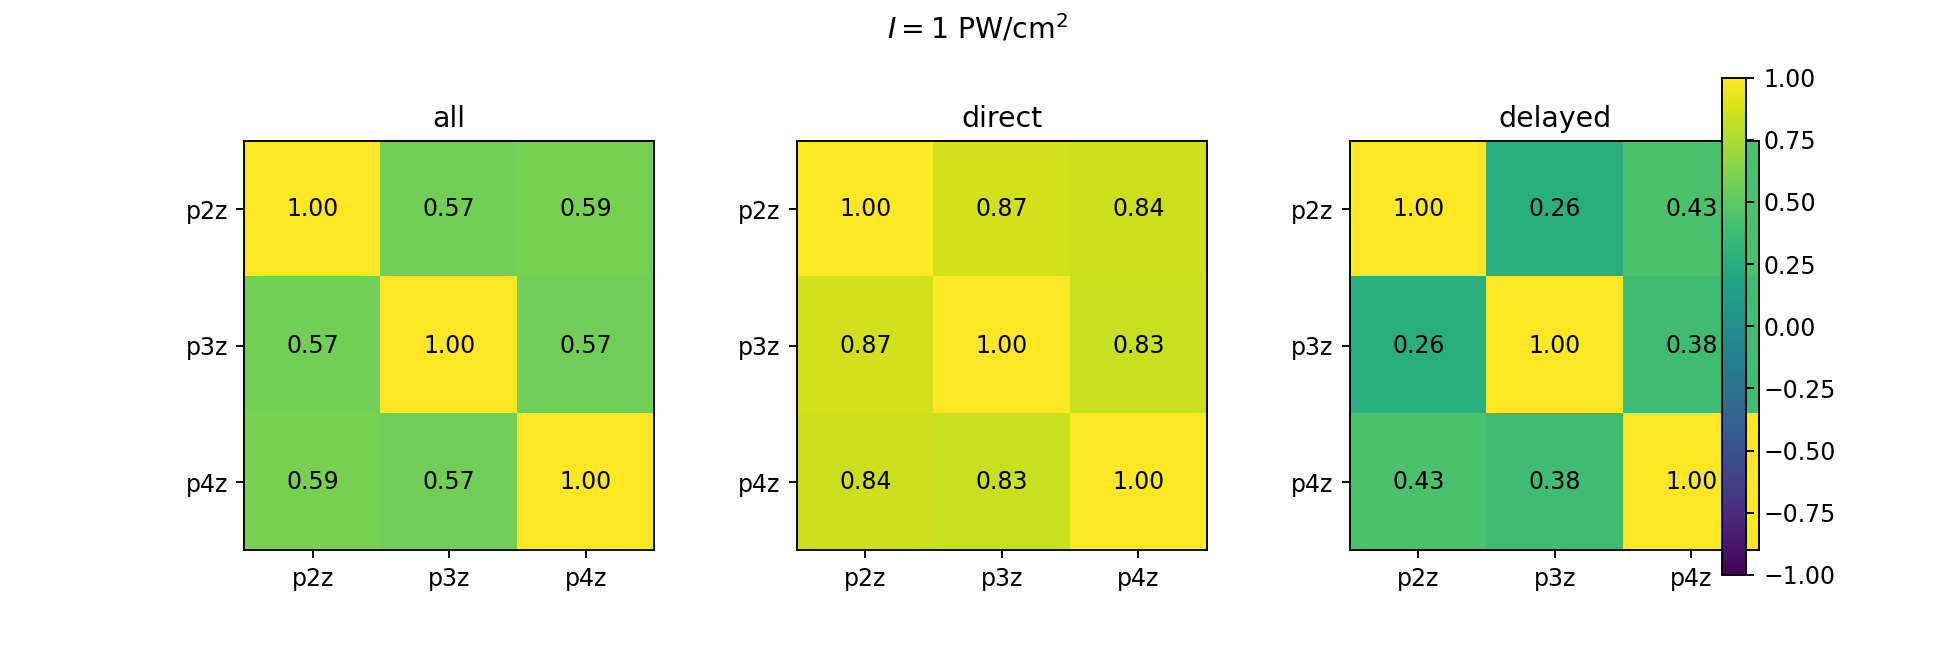
\includegraphics[width=0.95\textwidth]{correlations_1p0.png}\\[-2pt]
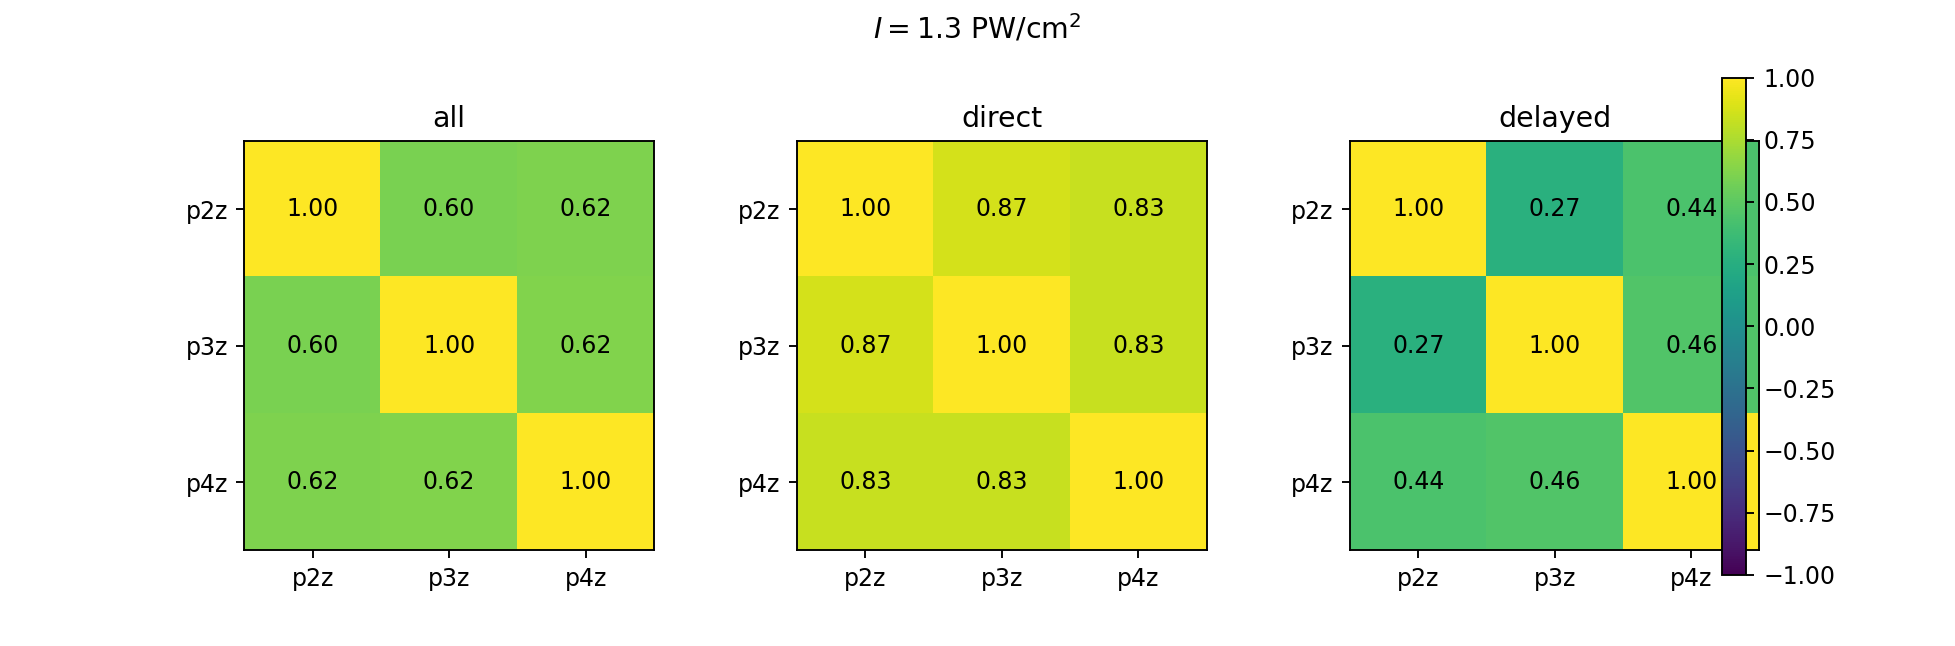
\includegraphics[width=0.95\textwidth]{correlations_1p3.png}\\[-2pt]
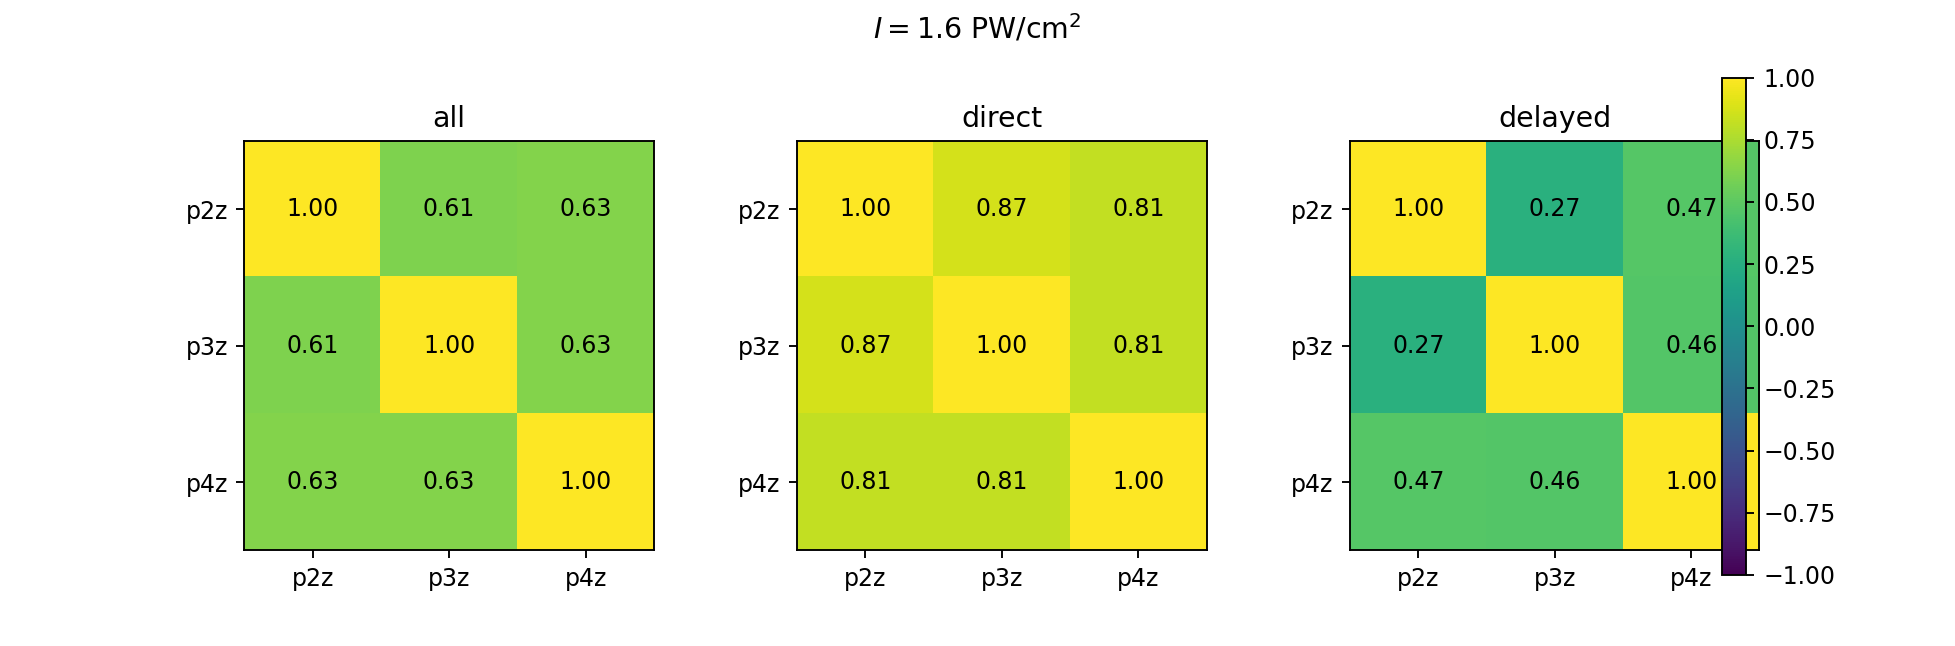
\includegraphics[width=0.95\textwidth]{correlations_1p6.png}\\[-2pt]
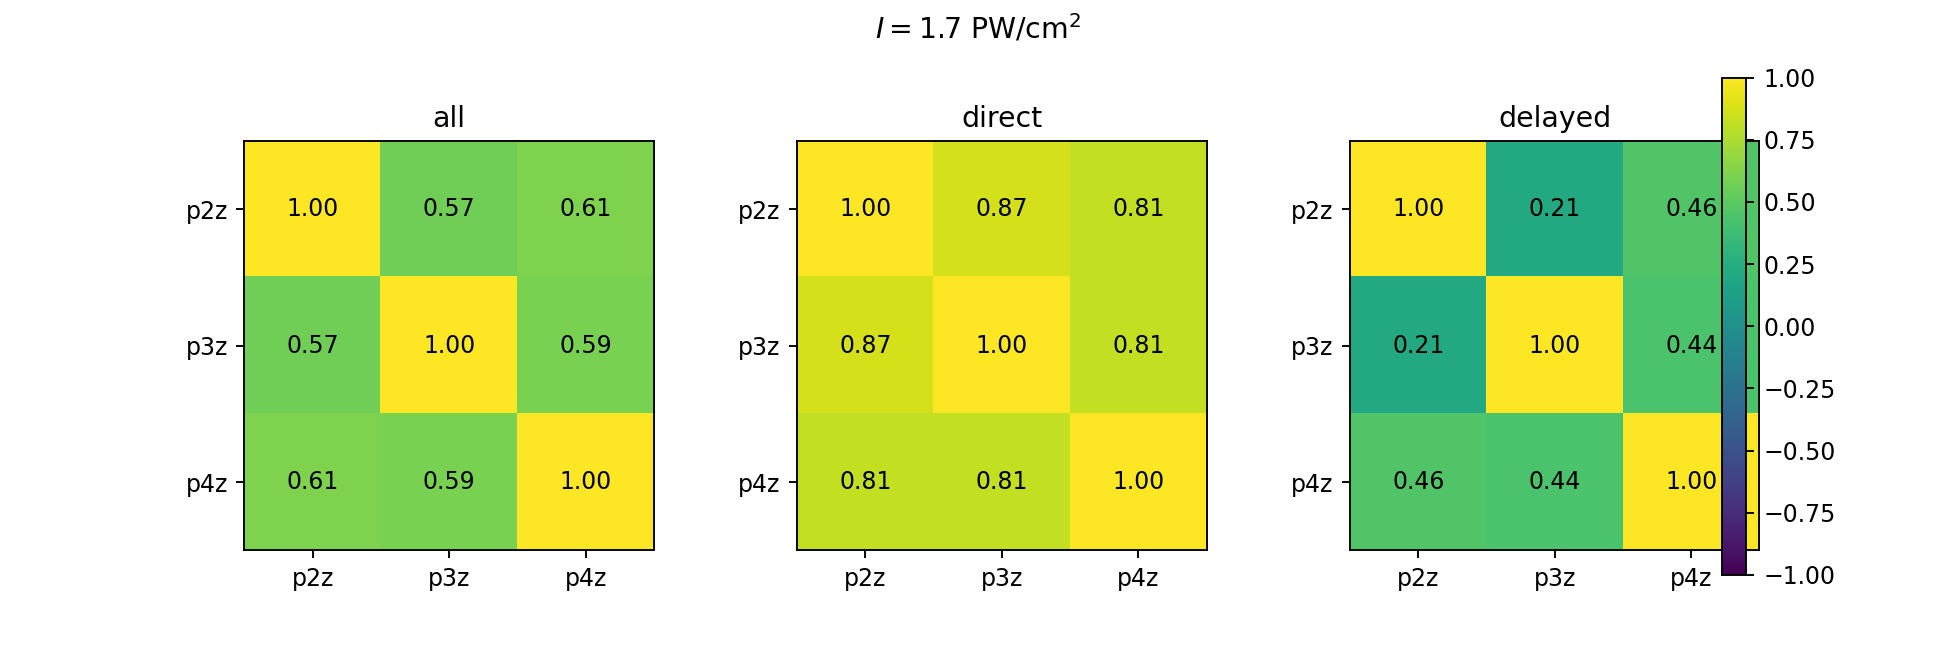
\includegraphics[width=0.95\textwidth]{correlations_1p7.png}
\caption{Macierze współczynników korelacji Pearsona dla pędów
podłużnych trzech elektronów. Kolejne wiersze odpowiadają
intensywnościom \num{1.0}, \num{1.3}, \num{1.6} i \num{1.7}~\PWcm,
a w każdym wierszu kolejne kolumny przedstawiają wszystkie zdarzenia,
kanał \emph{direct} i kanał \emph{delayed}. Ostatni wiersz dotyczy
innej długości fali.}
\label{fig:korelacje}
\end{figure}

\subsection{Zależność od intensywności pola}
\label{sec:wyn:intensywnosc}

Na koniec sprawdzono, jak wyniki zmieniają się w zależności od intensywności pola.
Seria o tej samej długości fali \num{800}~nm obejmuje zbiory \num{1.0},
\num{1.3} i \num{1.6}~\PWcm. Zbiór \num{1.7}~\PWcm{} policzono dla
długości fali \num{760}~nm, dlatego nie włączono go do serii
i omówiono osobno.

Dla każdej wielkości wyznaczono jej średnią w każdym zbiorze wraz
z niepewnością. Dla $\langle K\rangle$, $\langle K/A\rangle$
i $\langle\Neff\rangle$ jest to odchylenie standardowe średniej, a dla
średniej korelacji par $\langle r\rangle$ niepewność wyznaczona metodą
bootstrap~\cite{Efron1979} z \num{200} powtórzeń. Zależność od
intensywności w serii \num{800}~nm opisano ważoną regresją liniową
\begin{equation}
  y=a+b\,(I-I_0)
  \label{eq:trend}
\end{equation}
z wagami $1/\sigma^2$, gdzie $I_0=\num{1.3}$~\PWcm. Przesunięcie zmiennej
o $I_0$ sprawia, że $a$ jest wartością w środku serii, a nie
przedłużeniem prostej do $I=0$. Zbioru \num{1.7}~\PWcm{} nie włączono do
dopasowania. Współczynniki zestawiono w tabeli~\ref{tab:trend_fit}.

\begin{figure}[H]
\centering
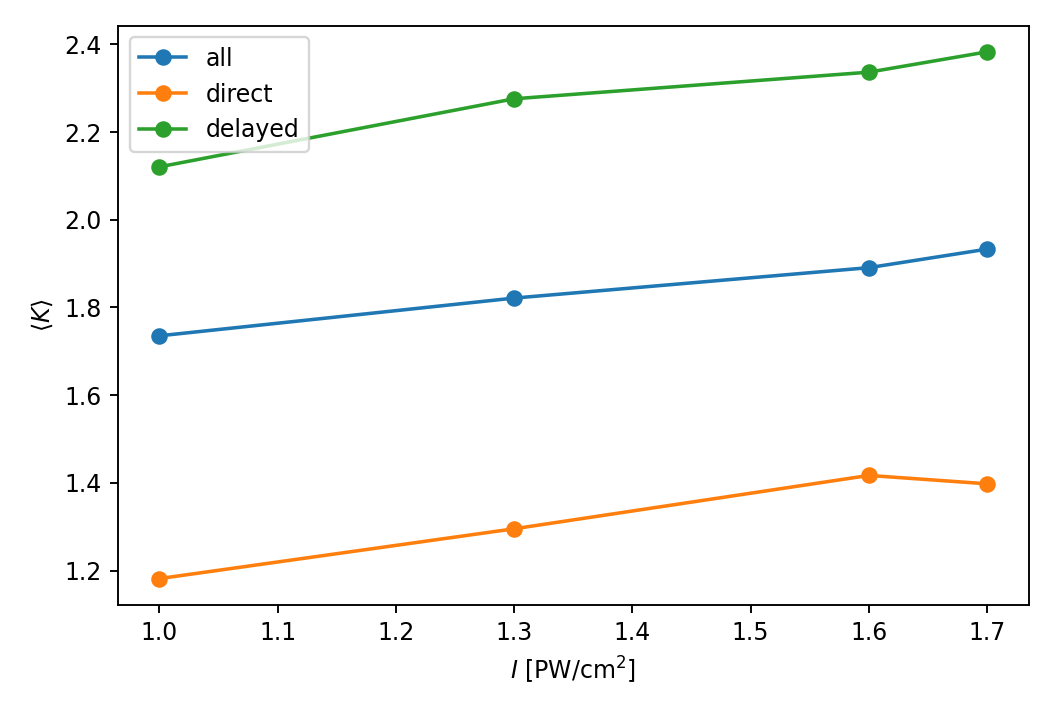
\includegraphics[width=0.8\textwidth]{trend_mean_K.png}
\caption{Zależność średniej skali nierównowagi $\langle K\rangle$ od
intensywności pola. Punkty przedstawiają wartości średnie
z niepewnościami, a linie ważone dopasowanie liniowe~\eqref{eq:trend}
do punktów serii \num{800}~nm, poza zakresem od \num{1.0} do
\num{1.6}~\PWcm{} są jego przedłużeniem. Pusty punkt przy
\num{1.7}~\PWcm{} odpowiada innej długości fali i nie wchodzi do
dopasowania.}
\label{fig:trend_K}
\end{figure}
Na rysunku~\ref{fig:trend_K} średnia skala nierównowagi
$\langle K\rangle$ rośnie w serii \num{800}~nm w obu kanałach, w kanale
\emph{direct} od \num{1.18} do \num{1.42}~\ja, a w kanale \emph{delayed}
od \num{2.12} do \num{2.34}~\ja{} (tabela~\ref{tab:glowna}). Wielkość $K$
ma jednak wymiar pędu, więc rośnie także wtedy, gdy wszystkie pędy
zwiększają się w tym samym stosunku, a sposób ich podziału pozostaje
bez zmian. Sam wzrost $\langle K\rangle$ nie pozwala więc stwierdzić,
czy zmienił się podział pędu. Aby oddzielić zmianę skali od zmiany
samego podziału, rozpatrzono stosunek $K/A$, gdzie $A$ jest sumą
wartości bezwzględnych pędów~\eqref{eq:udzialy}. Wielkość ta jest
bezwymiarowa i nie zmienia się, gdy wszystkie pędy rosną w tym samym
stosunku.

\begin{figure}[H]
\centering
\includegraphics[width=0.8\textwidth]{trend_mean_K_over_A.png}
\caption{Zależność średniego stosunku $\langle K/A\rangle$ od
intensywności pola. Oznaczenia jak na rysunku~\ref{fig:trend_K}.}
\label{fig:trend_KA}
\end{figure}

Na rysunku~\ref{fig:trend_KA} w kanale \emph{delayed} stosunek
$\langle K/A\rangle$ pozostaje stały i wynosi od \num{0.409} do
\num{0.411}, a nachylenie prostej $\num{0.001}\pm\num{0.006}$ na \PWcm{}
jest zgodne z zerem. Wzrost $\langle K\rangle$ wynika więc w tym kanale
wyłącznie ze wzrostu skali pędów. W kanale \emph{direct}
$\langle K/A\rangle$ rośnie od \num{0.196} do \num{0.218}, przy czym
większa część tej zmiany przypada na przedział od \num{1.3} do
\num{1.6}~\PWcm. W tym kanale zmienia się zatem również sam podział
pędu, który staje się mniej równomierny.

\begin{figure}[H]
\centering
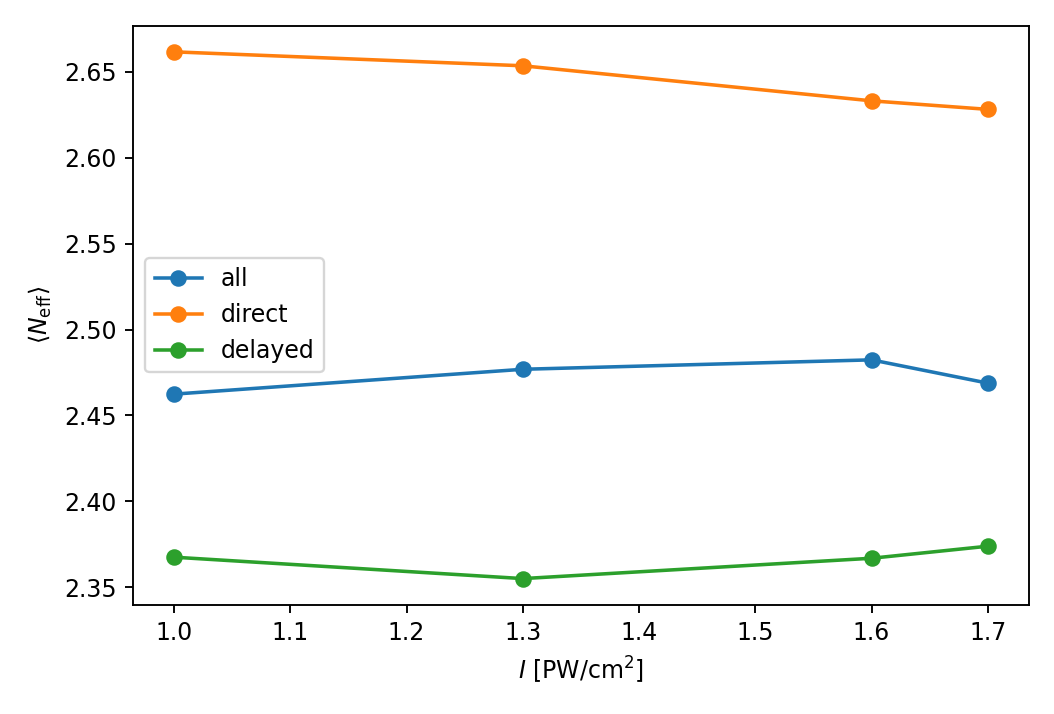
\includegraphics[width=0.8\textwidth]{trend_mean_N_eff.png}
\caption{Zależność średniej efektywnej liczby elektronów
$\langle\Neff\rangle$ od intensywności pola. Oznaczenia jak na
rysunku~\ref{fig:trend_K}.}
\label{fig:trend_neff}
\end{figure}

Ten sam obraz daje efektywna liczba elektronów
(rysunek~\ref{fig:trend_neff}). W kanale \emph{direct}
$\langle\Neff\rangle$ maleje od \num{2.662} do \num{2.633}, a nachylenie
wynosi $\num{-0.053}\pm\num{0.011}$ na \PWcm. W kanale \emph{delayed}
$\langle\Neff\rangle$ wynosi od \num{2.355} do \num{2.367} bez wyraźnego
kierunku zmian, a nachylenie $\num{0.009}\pm\num{0.015}$ na \PWcm{} jest
zgodne z zerem.

Zmiany wszystkich wielkości bezwymiarowych w serii \num{800}~nm
zestawiono w tabeli~\ref{tab:trend}. Oprócz $\langle\Neff\rangle$
i $\langle K/A\rangle$ podano w niej $\langle\xmax\rangle$, udział
zdarzeń o zgodnych znakach pędów $f_{\mathrm{zg}}$ oraz średni udział
pędu elektronu mniejszościowego $\langle x_{\mathrm{mn}}\rangle$
(tabela~\ref{tab:mniejszosc}). Istotność różnicy między zbiorami
\num{1.0} i \num{1.6}~\PWcm{} sprawdzono testem Welcha~\eqref{eq:welch}.
Wielkość $f_{\mathrm{zg}}$ jest średnią zmiennej przyjmującej wartość 1
dla zdarzenia z sektora zgodnego i 0 dla zdarzenia z sektora
mieszanego, dlatego przyjęto dla niej $s^2=f_{\mathrm{zg}}(1-f_{\mathrm{zg}})$.
Ponieważ wykonano dziesięć porównań, zastosowano poprawkę
Bonferroniego~\cite{Dunn1961} z progiem $\num{0.05}/10=\num{0.005}$.
\begin{table}[htbp]
  \centering
  \caption{Wielkości bezwymiarowe w serii \num{800}~nm oraz porównanie
  zbiorów \num{1.0} i \num{1.6}~\PWcm{} testem Welcha.
  $\Delta$ oznacza różnicę wartości przy \num{1.6} i \num{1.0}~\PWcm.}
  \label{tab:trend}
  \begin{tabular}{llcccccc}
    \toprule
    kanał & wielkość & \num{1.0} & \num{1.3} & \num{1.6} & $\Delta$ & $t$ & $p$ \\
    \midrule
    \emph{direct} & $\langle\Neff\rangle$           & \num{2.662} & \num{2.654} & \num{2.633} & \num{-0.029} & \num{-4.0}  & \num{7e-5} \\
                  & $\langle\xmax\rangle$           & \num{0.464} & \num{0.466} & \num{0.471} & \num{0.006}  & \num{3.3}   & \num{9e-4} \\
                  & $\langle K/A\rangle$            & \num{0.196} & \num{0.201} & \num{0.218} & \num{0.022}  & \num{8.0}   & \num{1e-15} \\
                  & $f_{\mathrm{zg}}$               & \num{0.974} & \num{0.953} & \num{0.908} & \num{-0.065} & \num{-13.9} & $<\num{1e-16}$ \\
                  & $\langle x_{\mathrm{mn}}\rangle$ & \num{0.070} & \num{0.116} & \num{0.166} & \num{0.096}  & \num{8.0}   & \num{1e-15} \\
    \midrule
    \emph{delayed} & $\langle\Neff\rangle$           & \num{2.367} & \num{2.355} & \num{2.367} & \num{-0.001} & \num{-0.1} & \num{0.95} \\
                   & $\langle\xmax\rangle$           & \num{0.530} & \num{0.535} & \num{0.536} & \num{0.005}  & \num{2.0}  & \num{0.046} \\
                   & $\langle K/A\rangle$            & \num{0.411} & \num{0.409} & \num{0.411} & \num{0.000}  & \num{-0.1} & \num{0.93} \\
                   & $f_{\mathrm{zg}}$               & \num{0.465} & \num{0.482} & \num{0.483} & \num{0.017}  & \num{1.4}  & \num{0.16} \\
                   & $\langle x_{\mathrm{mn}}\rangle$ & \num{0.177} & \num{0.187} & \num{0.210} & \num{0.033}  & \num{6.6}  & \num{4e-11} \\
    \bottomrule
  \end{tabular}
\end{table}

W kanale \emph{direct} zmiany wszystkich pięciu wielkości są istotne
i mają zgodny kierunek. Wartość $\langle\Neff\rangle$ maleje,
a $\langle\xmax\rangle$ i $\langle K/A\rangle$ rosną, więc podział pędu
staje się mniej równomierny. Jednocześnie $f_{\mathrm{zg}}$ maleje od
\num{0.974} do \num{0.908}, a $\langle x_{\mathrm{mn}}\rangle$ rośnie od
\num{0.070} do \num{0.166}. Coraz więcej zdarzeń opuszcza zatem sektory
zgodne, a elektron mniejszościowy niesie coraz większą część pędu.
W kanale \emph{delayed} istotnie zmienia się jedynie
$\langle x_{\mathrm{mn}}\rangle$, który rośnie od \num{0.177} do
\num{0.210}.

\begin{figure}[H]
\centering
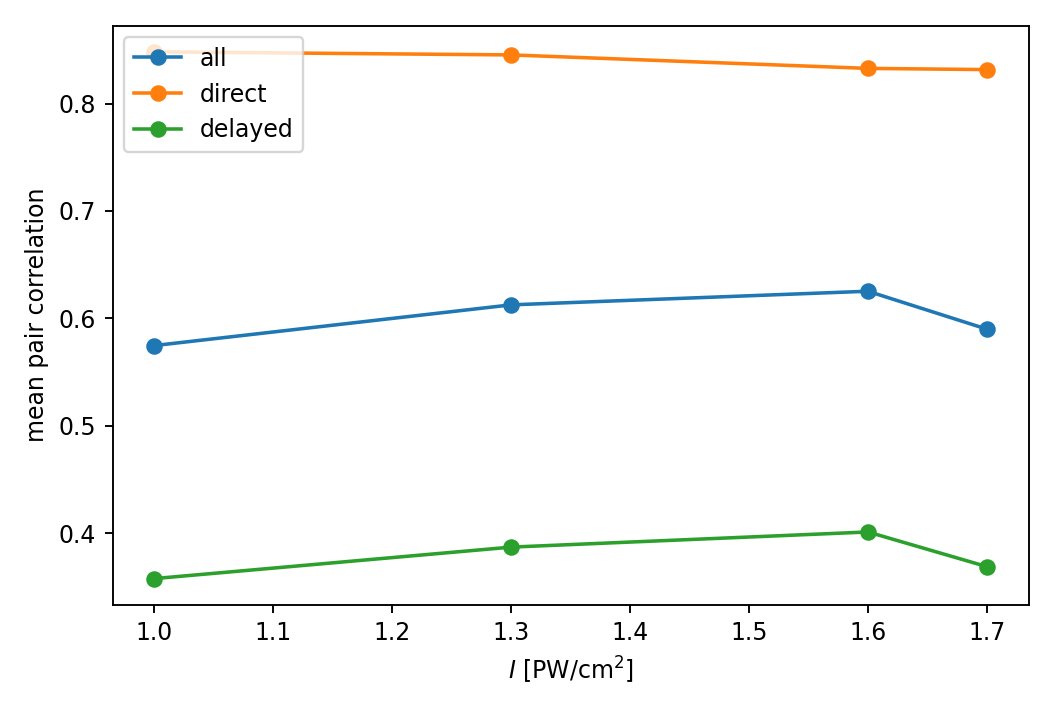
\includegraphics[width=0.8\textwidth]{trend_mean_pair_correlation.png}
\caption{Zależność średniej korelacji par pędów podłużnych
$\langle r\rangle$ od intensywności pola. Oznaczenia jak na
rysunku~\ref{fig:trend_K}.}
\label{fig:trend_r}
\end{figure}
Podobny obraz daje średnia korelacja par pędów podłużnych
$\langle r\rangle$, czyli średnia z trzech współczynników $r_{23}$,
$r_{24}$ i $r_{34}$ (rysunek~\ref{fig:trend_r}). W kanale \emph{direct}
maleje ona od \num{0.848} do \num{0.833}, a nachylenie prostej wynosi
$\num{-0.029}\pm\num{0.006}$ na \PWcm. W kanale \emph{delayed} rośnie od
\num{0.358} do \num{0.401}, z nachyleniem $\num{0.065}\pm\num{0.017}$ na
\PWcm. Różnicę między zbiorami \num{1.0} i \num{1.6}~\PWcm{} podzielono
przez jej niepewność wyznaczoną metodą bootstrap i otrzymano
$z=\num{-4.5}$ ($p=\num{8e-6}$) w kanale \emph{direct} oraz $z=\num{4.0}$
($p=\num{8e-5}$) w kanale \emph{delayed}. Spadek w kanale \emph{direct}
jest zgodny z malejącym udziałem zdarzeń, w których wszystkie elektrony
poruszają się w tę samą stronę.
Wartości dla wszystkich zdarzeń, widoczne na
rysunkach~\ref{fig:trend_K}--\ref{fig:trend_r}, nie są interpretowane
osobno. Zależą one od proporcji między kanałami, które zmieniają się
z intensywnością, a ponadto obejmują zdarzenia ścieżek rzadszych
(tabela~\ref{tab:licznosci}).
\begin{table}[htbp]
  \centering
  \caption{Współczynniki ważonej regresji liniowej~\eqref{eq:trend}
  dopasowanej do serii \num{800}~nm (\num{1.0}, \num{1.3}
  i \num{1.6}~\PWcm). Niepewności odpowiadają jednemu odchyleniu
  standardowemu. Współczynnik $b$ podano w jednostkach wielkości $y$ na
  \PWcm. Dopasowanie ma jeden stopień swobody.}
  \label{tab:trend_fit}
  \begin{tabular}{llccc}
    \toprule
    kanał & wielkość $y$ & $a$ & $b$ & $\chi^2$ \\
    \midrule
    wszystkie      & $\langle K\rangle$ [\ja] & $\num{1.817}\pm\num{0.006}$ & $\num{0.253}\pm\num{0.024}$  & \num{0.53} \\
                   & $\langle K/A\rangle$     & $\num{0.333}\pm\num{0.001}$ & $\num{-0.008}\pm\num{0.005}$ & \num{11.94} \\
                   & $\langle\Neff\rangle$    & $\num{2.475}\pm\num{0.002}$ & $\num{0.029}\pm\num{0.010}$  & \num{0.93} \\
                   & $\langle r\rangle$       & $\num{0.606}\pm\num{0.003}$ & $\num{0.071}\pm\num{0.011}$  & \num{6.30} \\
    \midrule
    \emph{direct}  & $\langle K\rangle$ [\ja] & $\num{1.298}\pm\num{0.005}$ & $\num{0.395}\pm\num{0.022}$  & \num{0.15} \\
                   & $\langle K/A\rangle$     & $\num{0.204}\pm\num{0.001}$ & $\num{0.041}\pm\num{0.004}$  & \num{9.08} \\
                   & $\langle\Neff\rangle$    & $\num{2.650}\pm\num{0.003}$ & $\num{-0.053}\pm\num{0.011}$ & \num{1.36} \\
                   & $\langle r\rangle$       & $\num{0.843}\pm\num{0.001}$ & $\num{-0.029}\pm\num{0.006}$ & \num{3.59} \\
    \midrule
    \emph{delayed} & $\langle K\rangle$ [\ja] & $\num{2.250}\pm\num{0.009}$ & $\num{0.329}\pm\num{0.038}$  & \num{6.88} \\
                   & $\langle K/A\rangle$     & $\num{0.410}\pm\num{0.001}$ & $\num{0.001}\pm\num{0.006}$  & \num{0.42} \\
                   & $\langle\Neff\rangle$    & $\num{2.362}\pm\num{0.003}$ & $\num{0.009}\pm\num{0.015}$  & \num{3.09} \\
                   & $\langle r\rangle$       & $\num{0.383}\pm\num{0.004}$ & $\num{0.065}\pm\num{0.017}$  & \num{0.89} \\
    \bottomrule
  \end{tabular}
\end{table}
Przy trzech punktach dopasowanie ma jeden stopień swobody, dlatego
zgodność z zależnością liniową oceniono statystyką $\chi^2$. Dla
$\langle K\rangle$ w kanale \emph{delayed}, $\langle K/A\rangle$
w kanale \emph{direct} oraz dla $\langle K/A\rangle$ i $\langle r\rangle$
wszystkich zdarzeń $\chi^2$ przekracza \num{3.84}, co odpowiada
$p<\num{0.05}$ i wskazuje na odstępstwo od zależności liniowej. W tych
przypadkach niepewności współczynników są zaniżone. Z tego powodu
o istotności zmian wnioskowano z bezpośredniego porównania zbiorów
\num{1.0} i \num{1.6}~\PWcm, a regresję traktowano jako opis kierunku
i wielkości zmian.
Wnioskując z otrzymanych wartości, zmiany wywołane intensywnością są
wielokrotnie mniejsze od różnicy między kanałami. Wartość
$\langle\Neff\rangle$ w kanale \emph{direct} zmienia się w całej serii
o \num{0.029}, podczas gdy różnica między kanałami wynosi od
\num{0.254} do \num{0.299} (tabela~\ref{tab:welch_neff}). Sposób podziału
pędu jest więc w rozpatrywanym zakresie przede wszystkim własnością
kanału, a intensywność zmienia głównie skalę pędów i proporcje między
kanałami (tabela~\ref{tab:licznosci}).

\subsection{Główne wyniki ilościowe}

Tabela~\ref{tab:glowna} zbiera wielkości omówione w
podrozdziałach~\ref{sec:wyn:Pe}--\ref{sec:wyn:intensywnosc} dla
wszystkich dwunastu zbiorów. Rolę elektronu mniejszościowego oraz
współczynniki korelacji par, jako wielkości zależne od numeracji,
zestawiono osobno w tabelach~\ref{tab:mniejszosc}
i~\ref{tab:korelacje}.

\begin{table}[!h]
\centering
\footnotesize
\setlength{\tabcolsep}{4pt}
\caption{Główne wyniki ilościowe dla analizowanych zbiorów.
Zapis $a\pm b$ oznacza wartość średnią $a$ oraz połowę szerokości
95-procentowego przedziału ufności $b$. Rozkład $P_e$ jest dwumodalny,
więc $\langle|P_e|\rangle$ podaje położenie maksimów, a
$\sigma(|P_e|)$ szerokość pojedynczego maksimum. Symbol
$f_{\mathrm{zg}}$ oznacza udział zdarzeń, w których wszystkie trzy
elektrony poruszają się w tę samą stronę. Wielkości
$\langle P_e\rangle$, $\langle|P_e|\rangle$, $\sigma(|P_e|)$ i
$\langle K\rangle$ podano w jednostkach atomowych. Zbiór
\num{1.7}~\PWcm{} policzono dla innej długości fali i nie należy on do
serii intensywności.}
\label{tab:glowna}
\begin{tabular}{c l c c c c c c c}
\toprule
 &  & \multicolumn{3}{c}{ruch kolektywny} & ruch względny
   & \multicolumn{3}{c}{obserwable bezwymiarowe} \\
\cmidrule(lr){3-5}
\cmidrule(lr){6-6}
\cmidrule(lr){7-9}
$I$ [\PWcm] & kanał & $\langle P_e\rangle$ & $\langle|P_e|\rangle$
  & $\sigma(|P_e|)$
  & $\langle K\rangle$ & $\langle\Neff\rangle$ & $\langle\xmax\rangle$
  & $f_{\mathrm{zg}}$ \\
\midrule
\num{1.0} & wszystkie & $\num{-0.080}\pm\num{0.152}$ & \num{4.943} & \num{2.194} & $\num{1.735}\pm\num{0.026}$ & $\num{2.462}\pm\num{0.011}$ & \num{0.512} & \num{0.647} \\
 & \emph{direct} & $\num{-0.073}\pm\num{0.289}$ & \num{6.466} & \num{1.582} & $\num{1.182}\pm\num{0.023}$ & $\num{2.662}\pm\num{0.012}$ & \num{0.464} & \num{0.974} \\
 & \emph{delayed} & $\num{-0.163}\pm\num{0.199}$ & \num{4.320} & \num{1.728} & $\num{2.121}\pm\num{0.040}$ & $\num{2.367}\pm\num{0.016}$ & \num{0.530} & \num{0.465} \\
\midrule
\num{1.3} & wszystkie & $\num{-0.012}\pm\num{0.102}$ & \num{5.560} & \num{2.502} & $\num{1.821}\pm\num{0.017}$ & $\num{2.477}\pm\num{0.007}$ & \num{0.508} & \num{0.669} \\
 & \emph{direct} & $\num{-0.124}\pm\num{0.183}$ & \num{7.064} & \num{1.964} & $\num{1.295}\pm\num{0.015}$ & $\num{2.654}\pm\num{0.008}$ & \num{0.466} & \num{0.953} \\
 & \emph{delayed} & $\num{0.080}\pm\num{0.134}$ & \num{4.799} & \num{2.058} & $\num{2.276}\pm\num{0.026}$ & $\num{2.355}\pm\num{0.010}$ & \num{0.535} & \num{0.482} \\
\midrule
\num{1.6} & wszystkie & $\num{-0.028}\pm\num{0.093}$ & \num{5.826} & \num{2.836} & $\num{1.891}\pm\num{0.015}$ & $\num{2.482}\pm\num{0.006}$ & \num{0.508} & \num{0.660} \\
 & \emph{direct} & $\num{-0.042}\pm\num{0.161}$ & \num{7.316} & \num{2.416} & $\num{1.417}\pm\num{0.014}$ & $\num{2.633}\pm\num{0.007}$ & \num{0.471} & \num{0.908} \\
 & \emph{delayed} & $\num{-0.021}\pm\num{0.124}$ & \num{4.961} & \num{2.397} & $\num{2.337}\pm\num{0.025}$ & $\num{2.367}\pm\num{0.009}$ & \num{0.536} & \num{0.483} \\
\midrule
\num{1.7} & wszystkie & $\num{0.183}\pm\num{0.197}$ & \num{5.601} & \num{2.770} & $\num{1.933}\pm\num{0.034}$ & $\num{2.469}\pm\num{0.013}$ & \num{0.512} & \num{0.632} \\
 & \emph{direct} & $\num{0.320}\pm\num{0.359}$ & \num{7.165} & \num{2.375} & $\num{1.398}\pm\num{0.032}$ & $\num{2.628}\pm\num{0.015}$ & \num{0.473} & \num{0.905} \\
 & \emph{delayed} & $\num{0.147}\pm\num{0.264}$ & \num{4.856} & \num{2.327} & $\num{2.383}\pm\num{0.056}$ & $\num{2.374}\pm\num{0.019}$ & \num{0.533} & \num{0.457} \\
\bottomrule
\end{tabular}
\end{table}


% ===========================================================================
\section{Porównanie z metodą simpleksową}
\label{sec:porownanie}
% ===========================================================================

Ponieważ obie metody, simpleksową oraz tą zaproponowaną w niniejszej pracy, zastosowano do tych samych danych, możliwe jest je
bezpośrednie porównanie. Wykorzystano przy tym tożsamość wykazaną
w podrozdziale~\ref{sec:zwiazek}, zgodnie z którą współrzędne
barycentryczne wykresu trójkątnego są udziałami $x_i$, a ściany
ośmiościanu sektorami znakowymi.

\subsection{Ilościowe sprawdzenie wniosków metody simpleksowej}

Reprezentację simpleksową dla wszystkich czterech intensywności
przedstawiono na rysunkach~\ref{fig:siatka_direct}
i~\ref{fig:siatka_delayed}, osobno dla każdego kanału.
\begin{figure}[H]
\centering
\includegraphics[width=0.8\textwidth]{siatka_1p0_direct.png}\\[0.2em]
\includegraphics[width=0.8\textwidth]{siatka_1p3_direct.png}\\[0.2em]
\includegraphics[width=0.8\textwidth]{siatka_1p6_direct.png}\\[0.2em]
\includegraphics[width=0.8\textwidth]{siatka_1p7_direct.png}
\caption{Siatka ośmiościanu dla kanału \emph{direct} bez symetryzacji.
Od góry kolejno \num{1.0}, \num{1.3}, \num{1.6} i \num{1.7}~\PWcm{}
(ostatni zbiór policzono dla \num{760}~nm). W każdej siatce lewa górna
ściana odpowiada sektorowi \texttt{+++}, a trzecia ściana w dolnym
rzędzie sektorowi \texttt{---}. Oznaczenia $p_{1z}$, $p_{2z}$, $p_{3z}$
na rysunkach odpowiadają pędom $p_2$, $p_3$, $p_4$ w tej pracy. Słupek
po prawej stronie każdego trójkąta podaje liczbę zliczeń. Rysunki
wykonano kodem towarzyszącym pracy~\cite{Ojczenasz2023}.}
\label{fig:siatka_direct}
\end{figure}
\begin{figure}[H]
\centering
\includegraphics[width=0.8\textwidth]{siatka_1p0_delayed.png}\\[0.2em]
\includegraphics[width=0.8\textwidth]{siatka_1p3_delayed.png}\\[0.2em]
\includegraphics[width=0.8\textwidth]{siatka_1p6_delayed.png}\\[0.2em]
\includegraphics[width=0.8\textwidth]{siatka_1p7_delayed.png}
\caption{Siatka ośmiościanu dla kanału \emph{delayed} bez symetryzacji.
Oznaczenia jak na rysunku~\ref{fig:siatka_direct}.}
\label{fig:siatka_delayed}
\end{figure}

Analiza simpleksowa danych~\cite{Ojczenasz2023} prowadziła do dwóch
wniosków jakościowych. Po pierwsze, przy emisji wszystkich trzech
elektronów w tę samą stronę punkty skupiają się w pobliżu środka
trójkąta, czyli pęd dzieli się w przybliżeniu równomiernie. Po drugie,
w sektorach mieszanych punkty skupiają się w pobliżu środka krawędzi,
czyli elektron poruszający się przeciwnie niesie niewielką część pędu.
Oba wnioski sprawdzono ilościowo, wyznaczając $\Neff$, $\xmax$
i najmniejszy udział $x_{\min}$ osobno dla sektorów zgodnych
i mieszanych. Wyniki dla wszystkich czterech intensywności zestawiono
w tabeli~\ref{tab:simpleks}.

\begin{table}[htbp]
\centering
\caption{Obserwable podziału pędu policzone osobno dla sektorów emisji
zgodnej i sektorów mieszanych. Środkowi trójkąta w metodzie simpleksowej  odpowiadają wartości
$\Neff=3$ i $\xmax=x_{\min}=1/3$, a środkowi krawędzi $\Neff=2$,
$\xmax=\num{0.5}$ i $x_{\min}=0$.}
\label{tab:simpleks}
\begin{tabular}{cclcccc}
\toprule
$I$ [\PWcm] & kanał & sektory & $n$ & $\langle\Neff\rangle$ &
$\langle\xmax\rangle$ & $\langle x_{\min}\rangle$ \\
\midrule
\num{1.0} & \emph{direct}  & zgodne   & \num{1988} & \num{2.676} & \num{0.461} & \num{0.206} \\
          & \emph{direct}  & mieszane & \num{54}   & \num{2.123} & \num{0.574} & \num{0.067} \\
          & \emph{delayed} & zgodne   & \num{976}  & \num{2.370} & \num{0.528} & \num{0.133} \\
          & \emph{delayed} & mieszane & \num{1121} & \num{2.366} & \num{0.532} & \num{0.136} \\
\midrule
\num{1.3} & \emph{direct}  & zgodne   & \num{5906} & \num{2.678} & \num{0.461} & \num{0.208} \\
          & \emph{direct}  & mieszane & \num{292}  & \num{2.164} & \num{0.569} & \num{0.084} \\
          & \emph{delayed} & zgodne   & \num{2815} & \num{2.384} & \num{0.526} & \num{0.138} \\
          & \emph{delayed} & mieszane & \num{3022} & \num{2.328} & \num{0.543} & \num{0.130} \\
\midrule
\num{1.6} & \emph{direct}  & zgodne   & \num{7992} & \num{2.673} & \num{0.461} & \num{0.207} \\
          & \emph{direct}  & mieszane & \num{807}  & \num{2.238} & \num{0.564} & \num{0.110} \\
          & \emph{delayed} & zgodne   & \num{3648} & \num{2.418} & \num{0.521} & \num{0.148} \\
          & \emph{delayed} & mieszane & \num{3912} & \num{2.319} & \num{0.549} & \num{0.133} \\
\midrule
\num{1.7} & \emph{direct}  & zgodne   & \num{1534} & \num{2.676} & \num{0.462} & \num{0.207} \\
          & \emph{direct}  & mieszane & \num{161}  & \num{2.177} & \num{0.580} & \num{0.101} \\
          & \emph{delayed} & zgodne   & \num{732}  & \num{2.421} & \num{0.519} & \num{0.149} \\
          & \emph{delayed} & mieszane & \num{869}  & \num{2.334} & \num{0.545} & \num{0.134} \\
\bottomrule
\end{tabular}
\end{table}

Drugi wniosek potwierdzono w obu kanałach. W sektorach mieszanych
kanału \emph{direct} $\langle\Neff\rangle$ wynosi od \num{2.123} do
\num{2.238}, a $\langle\xmax\rangle$ od \num{0.564} do \num{0.580}, czyli
wartości leżą blisko odniesienia dla środka krawędzi. Średni udział
pędu elektronu mniejszościowego wynosi w tym kanale od \num{0.070} do
\num{0.171}, a udział zdarzeń, w których jest on mniejszy od
\num{0.15}, od \num{0.599} do \num{0.852} (tabela~\ref{tab:mniejszosc}).
W kanale \emph{delayed} średni udział elektronu mniejszościowego jest
większy i wynosi od \num{0.177} do \num{0.210}, a mniejszy od \num{0.15}
jest on w \num{0.418}--\num{0.502} zdarzeń. Dla porównania, przy
udziałach rozłożonych jednorodnie na simpleksie udział wybranego
elektronu wynosi średnio $1/3$, a mniejszy od \num{0.15} jest
w $1-(1-\num{0.15})^2\approx\num{0.28}$ zdarzeń. W obu kanałach
elektron mniejszościowy niesie więc wyraźnie mniejszą część pędu niż
przy braku preferencji, a do wniosków otrzymanych z metody simpleksowej można teraz
dodać również konkretną liczbę.

Dla sektorów zgodnych obraz jest bardziej złożony. W kanale
\emph{direct} $\langle\Neff\rangle$ wynosi tam od \num{2.673} do
\num{2.678}, czyli wyraźnie więcej niż odniesienie \num{2.118}, ale
zauważalnie mniej niż wartość \num{3} odpowiadająca dokładnie równemu
podziałowi. Rozkład jest więc skupiony \emph{wokół} środka trójkąta,
ale ma skończoną szerokość, którą $\Neff$ mierzy bezpośrednio.
Określenie ,,w przybliżeniu równy podział'' jest zatem poprawne co do
kierunku, lecz nie rozróżnia przypadków istotnie różnych.
Widać to przy porównaniu kanałów w obrębie tych samych sektorów
zgodnych. W kanale \emph{delayed} $\langle\Neff\rangle$ wynosi tam od
\num{2.370} do \num{2.421}, mimo że oba zbiory leżą na tej samej ścianie
i na wykresie trójkątnym wyglądają jak skupienie wokół środka
(rysunek~\ref{fig:dalitz}). Różnicę między kanałami sprawdzono testem
Welcha~\eqref{eq:welch}, a wyniki zestawiono
w tabeli~\ref{tab:simpleks_welch}. W sektorach zgodnych różnica wynosi
od \num{0.254} do \num{0.307} przy $p<\num{1e-16}$, czyli jest tego
samego rzędu co różnica dla wszystkich zdarzeń
(tabela~\ref{tab:welch_neff}). W sektorach mieszanych kierunek różnicy
jest odwrotny, a zdarzenia kanału \emph{direct} leżą bliżej środka
krawędzi niż zdarzenia kanału \emph{delayed}. Obserwabla skalarna
rozdziela zatem przypadki, które w reprezentacji graficznej wymagałyby
wzrokowego porównania dwóch map gęstości.
\begin{table}[htbp]
  \centering
  \caption{Porównanie $\langle\Neff\rangle$ w kanałach \emph{direct}
  i \emph{delayed} osobno dla sektorów zgodnych i mieszanych testem
  Welcha.
  $\Delta=\langle\Neff\rangle_{\mathrm{direct}}-\langle\Neff\rangle_{\mathrm{delayed}}$
  oznacza różnicę średnich.}
  \label{tab:simpleks_welch}
  \begin{tabular}{ccccccc}
    \toprule
    & \multicolumn{3}{c}{sektory zgodne} & \multicolumn{3}{c}{sektory mieszane} \\
    \cmidrule(lr){2-4}\cmidrule(lr){5-7}
    $I$ [\PWcm] & $\Delta$ & $t$ & $p$ & $\Delta$ & $t$ & $p$ \\
    \midrule
    \num{1.0} & \num{0.307} & \num{22.8} & $<\num{1e-16}$ & \num{-0.242} & \num{-5.8} & \num{8e-9} \\
    \num{1.3} & \num{0.293} & \num{36.5} & $<\num{1e-16}$ & \num{-0.164} & \num{-8.2} & \num{2e-16} \\
    \num{1.6} & \num{0.255} & \num{35.9} & $<\num{1e-16}$ & \num{-0.081} & \num{-5.5} & \num{4e-8} \\
    \num{1.7} & \num{0.254} & \num{16.0} & $<\num{1e-16}$ & \num{-0.158} & \num{-4.8} & \num{2e-6} \\
    \bottomrule
  \end{tabular}
\end{table}


\subsection{Symetryzacja permutacyjna}

W metodzie simpleksowej stosuje się symetryzację, czyli powiększenie
zbioru danych o wszystkie permutacje etykiet elektronów. Jest to
uzasadnione ich nierozróżnialnością i wyraźnie poprawia czytelność
wykresu. Widoczna na rysunku~\ref{fig:dalitz} sześciokrotna symetria
obrazu jest bezpośrednim skutkiem tej operacji.
Dla obserwabli użytych w tej pracy zabieg ten jest zbędny. Wielkości
$\Neff$ i $\xmax$ są z definicji symetrycznymi funkcjami trójki
udziałów, więc symetryzacja nie może zmienić ich wartości. Sprawdzono
to bezpośrednio. Po rozszerzeniu zbioru o wszystkie sześć permutacji
średnie $\langle\Neff\rangle$ i $\langle\xmax\rangle$ różnią się od
pierwotnych o nie więcej niż \num{5.6e-17}
(podrozdział~\ref{sec:walidacja}). W podejściu graficznym symetryzacja
jest więc potrzebna, aby obraz był czytelny, natomiast tutaj
niezmienniczość względem permutacji wynika z samej definicji
obserwabli.
Symetryzacja ma jednak dodatkowy skutek. Usuwa ona z danych informację
o etykietach, a wraz z nią efekty opisane w
podrozdziałach~\ref{sec:wyn:sektory} i~\ref{sec:wyn:korelacje}. Po
symetryzacji nie można już stwierdzić, że elektron początkowo
tunelujący jest elektronem mniejszościowym w \num{0.205}--\num{0.235}
zdarzeń mieszanych kanału \emph{delayed} zamiast oczekiwanej $1/3$.
Rozdzielenie obserwabli na symetryczne i zależne od etykiet pozwala
korzystać z obu rodzajów informacji jednocześnie, przy czym
interpretacji fizycznej podlegają tylko obserwable symetryczne.

\subsection{Informacja dostępna w każdej z metod}
Obie metody opisują ten sam podział pędu bezwzględnego i tę samą
topologię znaków, ponieważ osiem ścian ośmiościanu odpowiada ośmiu
sektorom znakowym. Różnią się natomiast zakresem informacji, którą
można z nich odczytać.

Pierwsza różnica dotyczy skali pędów. Przy przejściu do udziałów $x_i$
pędy dzieli się przez ich sumę $A$, więc w reprezentacji simpleksowej
informacja o skali zostaje usunięta. Nie można z niej odczytać ani
całkowitego pędu $P_e$, ani skali nierównowagi $K$. W opisie skalarnym
obie te wielkości są dostępne obok udziałów, co pozwoliło
w podrozdziale~\ref{sec:wyn:intensywnosc} oddzielić zmianę skali od
zmiany samego podziału.

Druga różnica dotyczy porównywania zbiorów. W reprezentacji
simpleksowej polega ono na wzrokowym zestawieniu dwóch map gęstości,
a w opisie skalarnym na wyznaczeniu różnicy średnich i sprawdzeniu jej
istotności testem Welcha~\eqref{eq:welch}. Efekty zależne od numeracji
elektronów są w metodzie simpleksowej usuwane przez symetryzację,
natomiast w tej pracy mierzy się je osobno i traktuje jako informację
o modelu. Reprezentacja simpleksowa jest ponadto praktycznie
ograniczona do trzech elektronów, a obserwable skalarne można
zdefiniować dla dowolnej ich liczby, co omówiono w następnym
podrozdziale.

Reprezentacja simpleksowa ma nad opisem skalarnym jedną istotną
przewagę, ponieważ pokazuje pełny kształt rozkładu udziałów. Wielkości
$\Neff$ i $\xmax$ są jego rzutami, więc dwa różne rozkłady mogą
w zasadzie dać tę samą średnią. Z tego powodu w pracy podano nie tylko
wartości średnie, ale też pełne histogramy (rysunek~\ref{fig:neff})
oraz wartości rozdzielone według sektorów (tabela~\ref{tab:simpleks}).
Obie metody najlepiej traktować jako uzupełniające się. Wykres
trójkątny służy do rozpoznania struktury, a obserwable skalarne do jej
zmierzenia i porównania.


\subsection{Skalowalność}


Zasadnicza różnica ujawnia się przy zwiększaniu liczby elektronów. Dla
$N$ elektronów udziały $x_i$ tworzą simpleks o wymiarze $N-1$, czyli
trójkąt dla $N=3$, czworościan dla $N=4$ i obiekt czterowymiarowy dla
$N=5$. Równocześnie liczba sektorów znakowych rośnie jak $2^N$. Metoda
graficzna przestaje więc być praktyczna już dla czterech elektronów,
gdzie zamiast ośmiu trójkątów trzeba by analizować szesnaście brył
trójwymiarowych.

Opis użyty w tej pracy zachowuje przy tym swoją postać. Definicja
\begin{equation}
\Neff=\Big(\sum_{i=1}^{N}x_i^2\Big)^{-1},\qquad
x_i=\frac{|p_i|}{\sum_{j=1}^{N}|p_j|},
\label{eq:NeffN}
\end{equation}
obowiązuje dla dowolnego $N$, przy czym $1\le\Neff\le N$, a $\Neff$
nadal podaje efektywną liczbę elektronów uczestniczących w podziale
pędu. W ten sam sposób uogólnia się baza~\eqref{eq:baza}. Pełna
macierz Helmerta ma dla $N$ zmiennych jeden wiersz kolektywny
$(1,\dots,1)/\sqrt{N}$ i $N-1$ wierszy względnych~\cite{Lancaster1965},
przy czym $k$-ty wiersz względny zestawia $k$-tą zmienną ze średnią
poprzednich. Wielkości $P_e$ i $K$ zachowują wtedy definicje
\begin{equation}
P_e=\sum_{i=1}^{N}p_i,\qquad
K=\Big(\sum_{i=1}^{N}p_i^2-\frac{P_e^2}{N}\Big)^{1/2},
\label{eq:KN}
\end{equation}
gdzie druga równość wynika bezpośrednio z zachowania normy przy
przekształceniu ortogonalnym. Niezależnie od $N$ wszystkie te
wielkości pozostają liczbami, które można przedstawić na histogramie
i porównywać między zbiorami testem Welcha, tak jak w
rozdziale~\ref{sec:wyniki}.
Skalowalność ta została jednak w niniejszej pracy wykazana wyłącznie
formalnie. Dostępne dane dotyczą trzech elektronów, więc przydatność
tych obserwabli dla $N\ge4$ nie została sprawdzona empirycznie.


% ===========================================================================
\section{Ograniczenia analizy}
\label{sec:ograniczenia}
% ===========================================================================

Poniżej zebrano ograniczenia, o których należy pamiętać przy
odczytywaniu wyników.

\paragraph{Charakter danych.} Analizowane pędy pochodzą z modelu
półklasycznego, nie z pomiaru. Model ten dobrze odtwarza mierzone widma
pędów~\cite{Emmanouilidou2023}, ale nie zawiera interferencji
kwantowych. Wszystkie wnioski dotyczą zatem w pierwszej kolejności
własności modelu.

\paragraph{Etykiety elektronów.} Podział na elektrony początkowo
związane i początkowo tunelujący oraz przypisanie zdarzenia do
kanału \emph{direct} albo \emph{delayed} są konstrukcjami modelu.
Wielkości od nich zależne, przede wszystkim analiza elektronu
mniejszościowego oraz porównanie $r_{23}$ z $r_{24}$ i $r_{34}$, opisują
strukturę modelu, a nie bezpośrednio obserwable kwantowe.

\paragraph{Zachowanie pędu.} Jak pokazano w
podrozdziale~\ref{sec:walidacja}, suma pędów podłużnych czterech
cząstek ma wartość średnią zgodną z zerem, ale rozrzut rzędu
\num{1.6}~\ja Nie pozwala to używać warunku zachowania pędu jako
testu dla pojedynczego zdarzenia. Przyczyna tego rozrzutu nie została w tej
pracy ustalona; jej wyjaśnienie wymagałoby dostępu do szczegółów
procedury numerycznej użytej przy generowaniu danych.

\paragraph{Zakres zmienności.} Seria intensywności obejmuje tylko trzy
punkty przy \num{800}~nm, w wąskim zakresie od \num{1.0} do
\num{1.6}~\PWcm. Wnioski o trendach należy traktować jako opis tego
zakresu. Zbioru \num{1.7}~\PWcm{} nie włączono do serii ze względu na
inną długość fali.

\paragraph{Zakres obserwabli.} Analizowano wyłącznie składowe
podłużne. Składowe poprzeczne niosą informację o geometrii
rekolizji, która nie została tu wykorzystana. Współczynnik korelacji
Pearsona opisuje jedynie zależności liniowe między parami i nie
wyczerpuje opisu korelacji trójelektronowych.

\paragraph{Niepewności.} Podane przedziały ufności uwzględniają
wyłącznie skończoną liczbę zdarzeń. Nie obejmują
niepewności parametrów modelu ani niepewności związanej z
przypisaniem zdarzeń do kanałów.

% ===========================================================================
\section{Podsumowanie}
% ===========================================================================

W pracy zaproponowano i sprawdzono sposób opisu podziału pędu
pomiędzy trzy elektrony uwalniane w niesekwencyjnej potrójnej jonizacji
neonu. Opis składa się z dwóch elementów: stałej bazy ortonormalnej
rozdzielającej ruch kolektywny $P_e$ od ruchu względnego
$(\xi_1,\xi_2)$ oraz zestawu bezwymiarowych obserwabli podziału pędu,
przede wszystkim efektywnej liczby elektronów $\Neff$.

Najważniejsze wyniki są następujące.

\begin{enumerate}
  \item Bazę wybrano na podstawie analizy składowych głównych, ale
        nie utożsamiono jej z osiami PCA. Pokazano, że PCA jednoznacznie
        wskazuje kierunek kolektywny (zgodność z $(1,1,1)/\sqrt3$ na
        poziomie \num{0.99997}), natomiast nie wyznacza jednoznacznie
        poszczególnych osi względnych, ponieważ odpowiadaję im
        wartości własne są bliskie.
  \item Transformacja jest obrotem, a nie redukcją wymiaru. Potwierdzono
        to numerycznie: zachowanie normy i odtworzenie składowych
        z dokładnością do \num{3.2e-14}.
  \item Obserwable $\Neff$ i $\xmax$ rozdzielają kanały \emph{direct}
        i \emph{delayed} przy każdej intensywności. Przy \num{1.3}~\PWcm{}
        $\langle\Neff\rangle$ wynosi \num{2.654} wobec \num{2.355}
        ($p<\num{1e-16}$). Obie wartości leżą powyżej odniesienia
        \num{2.118} odpowiadającego brakowi preferencji.
  \item Spójny obraz obu kanałów dają również pozostałe
        obserwable: udział emisji w tę samą stronę
        (\num{0.953} wobec \num{0.482}) oraz korelacje par
        ($\approx\num{0.85}$ wobec $\num{0.27}$--$\num{0.46}$).
  \item Obserwable bezwymiarowe są niemal niezależne od intensywności
        w badanym zakresie, natomiast silnie zależą od kanału.
        Sposób podziału pędu jest więc własnością
        ścieżki jonizacji.
  \item Wykazano, że reprezentacja simpleksowa i opis skalarny operują
        na tym samym obiekcie matematycznym. Pozwoliło to sprawdzić
        ilościowo wnioski uzyskane wcześniej metodą simpleksową.
        Oba zostały potwierdzone co do kierunku, ale opis skalarny wykazał
        dodatkowo, że skupienie wokół środka trójkąta ma
        różną szerokość w obu kanałach (\num{2.678} wobec
        \num{2.384} przy \num{1.3}~\PWcm), czego sam obraz graficzny nie
        rozdziela.
  \item Obserwable skalarne są z definicji niezmiennicze względem
        permutacji etykiet, co sprawdzono numerycznie. Dzięki temu nie
        wymagają symetryzacji zbioru danych i pozwalają analizować
        efekty zależne od etykiet osobno, zamiast je usuwać.
  \item Opis zachowuje swój kształt dla dowolnej liczby elektronów,
        co pokazano formalnie. Empiryczne sprawdzenie dla $N\ge4$ wymaga
        danych, które nie były dostępne.
\end{enumerate}

Naturalnym kierunkiem dalszej pracy jest zastosowanie tych obserwabli do
danych dla czterech elektronów, gdzie metoda simpleksowa nie jest już
użyteczna, oraz uwzględnienie składowych poprzecznych pędu.

% ===========================================================================
\appendix
\section{Elektron mniejszościowy w sektorach mieszanych}
% ===========================================================================

\begin{table}[H]
\centering
\small
\caption{Rola elektronu mniejszościowego w sektorach mieszanych. Kolumna
$f_4$ podaje udział zdarzeń, w których elektronem mniejszościowym jest
elektron początkowo tunelujący; przy równoważnych etykietach
oczekiwano by \num{0.333}. Kolumna $\langle x_{\mathrm{mn}}\rangle$ podaje
średni udział pędu tego elektronu.}
\label{tab:mniejszosc}
\begin{tabular}{clccccc}
\toprule
$I$ [\PWcm] & kanał & $n_{\mathrm{miesz}}$ & $f_4$ &
$\langle x_{\mathrm{mn}}\rangle$ & mediana $x_{\mathrm{mn}}$ &
$P(x_{\mathrm{mn}}<\num{0.15})$ \\
\midrule
\num{1.0} & \emph{direct}  & \num{54}   & \num{0.370}\,$\pm$\,\num{0.066} & \num{0.070} & \num{0.048} & \num{0.852} \\
\num{1.0} & \emph{delayed} & \num{1121} & \num{0.234}\,$\pm$\,\num{0.013} & \num{0.177} & \num{0.149} & \num{0.502} \\
\num{1.3} & \emph{direct}  & \num{292}  & \num{0.534}\,$\pm$\,\num{0.029} & \num{0.116} & \num{0.074} & \num{0.747} \\
\num{1.3} & \emph{delayed} & \num{3022} & \num{0.225}\,$\pm$\,\num{0.008} & \num{0.187} & \num{0.151} & \num{0.498} \\
\num{1.6} & \emph{direct}  & \num{807}  & \num{0.545}\,$\pm$\,\num{0.018} & \num{0.166} & \num{0.119} & \num{0.599} \\
\num{1.6} & \emph{delayed} & \num{3912} & \num{0.235}\,$\pm$\,\num{0.007} & \num{0.210} & \num{0.171} & \num{0.441} \\
\num{1.7} & \emph{direct}  & \num{161}  & \num{0.534}\,$\pm$\,\num{0.039} & \num{0.171} & \num{0.121} & \num{0.609} \\
\num{1.7} & \emph{delayed} & \num{869}  & \num{0.205}\,$\pm$\,\num{0.014} & \num{0.209} & \num{0.174} & \num{0.418} \\
\bottomrule
\end{tabular}
\end{table}

\section{Korelacje par pędów podłużnych}

\begin{table}[htbp]
  \centering
  \small
  \caption{Współczynniki korelacji Pearsona $r_{ij}$~\eqref{eq:pearson}
  między pędami podłużnymi par elektronów wraz z 95-procentowymi
  przedziałami ufności $[r_{ij}^{(\num{0.025})};\,r_{ij}^{(\num{0.975})}]$
  wyznaczonymi transformacją Fishera.}
  \label{tab:korelacje}
  \begin{tabular}{llcccccc}
    \toprule
    $I$ [\PWcm] & kanał
      & $r_{23}$ & $[r_{23}^{(\num{0.025})};\,r_{23}^{(\num{0.975})}]$
      & $r_{24}$ & $[r_{24}^{(\num{0.025})};\,r_{24}^{(\num{0.975})}]$
      & $r_{34}$ & $[r_{34}^{(\num{0.025})};\,r_{34}^{(\num{0.975})}]$ \\
    \midrule
    \num{1.0} & \emph{direct}  & \num{0.867} & $[\num{0.856};\,\num{0.877}]$ & \num{0.844} & $[\num{0.831};\,\num{0.856}]$ & \num{0.833} & $[\num{0.819};\,\num{0.846}]$ \\
              & \emph{delayed} & \num{0.263} & $[\num{0.222};\,\num{0.302}]$ & \num{0.428} & $[\num{0.393};\,\num{0.463}]$ & \num{0.382} & $[\num{0.345};\,\num{0.418}]$ \\
    \midrule
    \num{1.3} & \emph{direct}  & \num{0.871} & $[\num{0.865};\,\num{0.877}]$ & \num{0.830} & $[\num{0.822};\,\num{0.838}]$ & \num{0.834} & $[\num{0.827};\,\num{0.842}]$ \\
              & \emph{delayed} & \num{0.268} & $[\num{0.244};\,\num{0.291}]$ & \num{0.435} & $[\num{0.414};\,\num{0.456}]$ & \num{0.459} & $[\num{0.438};\,\num{0.479}]$ \\
    \midrule
    \num{1.6} & \emph{direct}  & \num{0.872} & $[\num{0.867};\,\num{0.877}]$ & \num{0.813} & $[\num{0.806};\,\num{0.820}]$ & \num{0.813} & $[\num{0.806};\,\num{0.820}]$ \\
              & \emph{delayed} & \num{0.269} & $[\num{0.248};\,\num{0.290}]$ & \num{0.470} & $[\num{0.452};\,\num{0.487}]$ & \num{0.465} & $[\num{0.447};\,\num{0.482}]$ \\
    \midrule
    \num{1.7} & \emph{direct}  & \num{0.868} & $[\num{0.856};\,\num{0.879}]$ & \num{0.813} & $[\num{0.796};\,\num{0.828}]$ & \num{0.814} & $[\num{0.797};\,\num{0.829}]$ \\
              & \emph{delayed} & \num{0.214} & $[\num{0.166};\,\num{0.260}]$ & \num{0.456} & $[\num{0.416};\,\num{0.494}]$ & \num{0.437} & $[\num{0.397};\,\num{0.476}]$ \\
    \bottomrule
  \end{tabular}
\end{table}

\section{Przebieg obliczeń}

Obliczenia wykonano w dwóch etapach, odpowiadających dwóm notatnikom
dołączonym do pracy.

\begin{enumerate}
  \item \texttt{05\_PCA\_full.ipynb} -- wczytanie dwunastu zbiorów,
        standaryzacja dziewięciu składowych pędu, analiza
        składowych głównych, zapis tabel wariancji wyjaśnionej,
        współczynników podłużnych oraz ich zgodności z kierunkami
        stałej bazy do katalogu \texttt{PCA\_results}.
  \item \texttt{07\_analiza\_3D\_clean.ipynb} -- wyznaczenie
        współrzędnych $Q$, $\xi_1$, $\xi_2$, obserwabli $K$, $A$,
        $x_i$, $\Neff$, $\xmax$, sektorów znakowych i korelacji,
        testy poprawności oraz zapis tabel i rysunków do katalogu
        \texttt{momentum\_sharing\_results}.
\end{enumerate}

Oba notatniki wykonują się od czystego jądra bez błędów.
Wszystkie wartości liczbowe przytoczone w tekście odtworzono dodatkowo
niezależną implementacją w języku Python korzystającą
wyłącznie z biblioteki standardowej, która również wyznacza
przedziały ufności, statystyki testów Welcha oraz wartości
odniesienia dla rozkładu równomiernego na simpleksie.

% ===========================================================================
\bibliographystyle{unsrt}
\bibliography{bibliography}
% ===========================================================================

\end{document}
